\documentclass[11pt,a4paper]{article}

\usepackage[utf8]{inputenc}
\usepackage[T1]{fontenc}
\usepackage{lmodern}
\DeclareUnicodeCharacter{0151}{\H{o}}
\DeclareUnicodeCharacter{0150}{\H{O}}
\DeclareUnicodeCharacter{0171}{\H{u}}
\DeclareUnicodeCharacter{0170}{\H{U}}
\usepackage[a4paper,margin=0.82in]{geometry}
\usepackage{amsmath,amssymb,amsthm}
\usepackage{booktabs}
\usepackage{longtable}
\usepackage{array}
\usepackage{graphicx}
\usepackage{xcolor}
\usepackage{hyperref}

\renewcommand{\contentsname}{Tartalomjegyz\'ek}
\renewcommand{\figurename}{\'Abra}
\renewcommand{\tablename}{T\'abl\'azat}
\renewcommand{\abstractname}{\"Osszefoglal\'o}
\renewcommand{\refname}{Irodalomjegyz\'ek}
\renewcommand{\proofname}{Bizony\'it\'as}

\hypersetup{
    colorlinks=true,
    linkcolor=blue!70!black,
    citecolor=blue!70!black,
    urlcolor=blue!70!black,
    pdftitle={Fekete lyukak, a Nagy Bumm es a jelenlegi kozmikus tagulas mint a diszkret K4 idobeli szubsztratum dualis Painleve-Gullstrand-rezsimjei},
    pdfauthor={Jolcsak, A. (Tau Core Research Collaboration)}
}

\setlength{\emergencystretch}{2.5em}
\newcolumntype{L}[1]{>{\raggedright\arraybackslash}p{#1}}
\newcolumntype{C}[1]{>{\centering\arraybackslash}p{#1}}
\newcolumntype{R}[1]{>{\raggedleft\arraybackslash}p{#1}}

\newtheorem{theorem}{T\'etel}[section]
\newtheorem{proposition}[theorem]{\'All\'it\'as}
\newtheorem{corollary}[theorem]{K\"ovetkezm\'eny}
\theoremstyle{remark}
\newtheorem{remark}[theorem]{Megjegyz\'es}

\title{\textbf{Fekete lyukak, a Nagy Bumm \'es a jelenlegi kozmikus t\'agul\'as mint a diszkr\'et $K_4$ id\H{o}beli szubsztr\'atum du\'alis Painlev\'e--Gullstrand-rezsimjei:\\
szingularit\'asmentes anat\'omia, horizont-termodinamika \'es t\"obbcsatorn\'as megfigyel\'esi valid\'aci\'o ($k = 0$)}}

\author{Jolcsak, A.\\
\small\textit{Tau Core Research Collaboration} (\texttt{tau-core-black-hole-cosmology-duality-paper21})}

\date{2026.\ november 14.}

\begin{document}
\maketitle

\begin{abstract}
\noindent
Az \'altal\'anos relativit\'aselm\'elet (GR) \'es a standard $\Lambda$ hideg s\"ot\'et anyag ($\Lambda\mathrm{CDM}$) kozmol\'ogiai modell a gravit\'aci\'ofizika hat alapvet\H{o} anom\'ali\'aj\'at --- (i) a fekete lyukak k\"ozponti g\"orb\"uleti szingularit\'as\'at ($r \to 0$) \'es a bels\H{o} Cauchy-horizont t\"omeginfl\'aci\'os instabilit\'as\'at, (ii) a kezdeti Nagy Bumm szingularit\'ast ($a \to 0$), (iii) a $10^{122}$ nagys\'agrend\H{u} kvantumv\'akuum kozmol\'ogiai-\'alland\'o katasztr\'of\'at, (iv) Penrose kezdeti Weyl-g\"orb\"uleti \'es m\'ultbeli entr\'opia-paradoxon\'at, (v) a galaktikus \'es halmazl\'ept\'ek\H{u} ,,s\"ot\'et anyag'' kinematik\'at \'es lencs\'ez\'est, valamint (vi) a k\'es\H{o}i kozmikus ,,s\"ot\'et energia'' gyorsul\'ast --- logikailag f\"uggetlen rejt\'elyekk\'ent kezeli, amelyek mind k\"ul\"on ad-hoc feltev\'eseket ig\'enyelnek. Jelen tanulm\'anyban analitikusan bizony\'itjuk (\texttt{SymPy} szimbolikus ellen\H{o}rz\'essel) \'es t\"obbcsatorn\'as er\H{o}s-teri, illetve kozmol\'ogiai m\'er\'eseken valid\'aljuk, hogy a forr\'as-befagyasztott \textbf{Tau Core H\'arompill\'eres Kanonikus Szint\'ezis ($k = 0$ szabadon hangolt param\'eter)} keret\'eben a fekete lyukak bels\H{o} szerkezete \'es a kozmikus t\'agul\'as egyetlen diszkr\'et $K_4$ pregeometriai szimplex \'altal vez\'erelt Painlev\'e--Gullstrand (PG) akusztikus \'ora-folyad\'ek egzakt el\H{o}jel-ford\'itott rezsimjeik\'ent ($\sigma_{\mathrm{flow}} = -1$, illetve $\sigma_{\mathrm{flow}} = +1$) jelennek meg.

Konkr\'etan \"ot egzakt t\'etelt (\texttt{D1--D5.\ t\'etelek}) vezet\"unk le:
\textbf{(D1)} Az euklideszi t\'erszeletekkel, $\dot{r}_\pm = c(\pm 1 + \sigma_{\mathrm{flow}}\beta)$ radi\'alis f\'enyk\'up-sebess\'egekkel, $g_{0r}(1/4) = -\sqrt{5}/8 \approx -0.27951$ bet\"olt\"ott cs\'iramag-eltol\'assal \'es konnekci\'omentes Cartan--Kodama $\mathrm{d}K$ k\"uls\H{o} 2-forma holon\'omi\'aval b\'ir\'o egyes\'itett PG-metrika stacion\'arius fekete lyukakra ($\sigma_{\mathrm{flow}} = -1$) a $\kappa_{\mathrm{BH}} = c^2/(2r_s)$, m\'ig a t\'agul\'o Univerzumra ($\sigma_{\mathrm{flow}} = +1$) a $|\kappa_{\mathrm{KH}}(z)| = \frac{1}{2}cH(z)|1 - q(z)| = cH(z)|1 - \frac{3}{4}\Omega_m(z)|$ fel\"uleti gravit\'aci\'ot adja.
\textbf{(D2)} T\'erben lapos, nyom\'asmentes anyagb\'ol \'es $\Lambda$-aszimptotik\'ab\'ol \'all\'o FLRW-kozmol\'ogi\'aban a jelenlegi kozmikus gyorsul\'as beindul\'asa $q(z_{\mathrm{acc}}) = 0$ ($\ddot{a} = 0$) \'es a galaktikus Kodama--Hayward-gyorsul\'assk\'ala minimuma $\mathrm{d}a_0^{\mathrm{KH}}/\mathrm{d}z = 0$ \emph{analitikusan pontosan ugyanabban a kozmikus korszakban}, $\Omega_m(z) = 2/3$ \'ert\'ekn\'el k\"ovetkezik be: $z_{\mathrm{acc}} \equiv z_{\mathrm{dip}} = (2\Omega_{\Lambda,0}/\Omega_{m,0})^{1/3} - 1 = 0.63155650$ ($a_0^{\mathrm{KH}}(z_{\mathrm{dip}})/a_0^{\mathrm{KH}}(0) = 0.93855026$).
\textbf{(D3--D4)} Az $r < r_s$ esem\'enyhorizonton bel\"ul a gravit\'aci\'os kollapszus n\'egy regul\'aris koncentrikus z\'on\'an halad \'at: szuperszonikus PG-zuhan\'as nyommentes $+2:-1:-1$ \texttt{CHDF} Weyl-\'arap\'alyny\'ujt\'assal (\textbf{I.\ z\'ona}), r\"ovid hat\'ot\'av\'u \texttt{COCA-H1} Yukawa-kivon\'as az $1/r^2$ szingularit\'as kiolt\'as\'aval ($+\frac{1}{2}GM m_{\mathrm{COCA}}^2$ v\'eges mag-er\H{o}) \'es kir\'alis 48-Weyl dekonfin\'aci\'oval (\textbf{II.\ z\'ona}), 15-csatorn\'as \texttt{CHDF} UV-nyomkiolt\'as $\mathrm{Tr}(T_{\mathrm{def}}^{(15)}) = 0$ a Cauchy-horizont f\'ekez\'es\'ere ($x_- \approx 0.0323$) $\pi_2(S^2) = \mathbb{Z}$ spin-text\'ur\'aval (\textbf{III.\ z\'ona}), v\'eg\"ul a Clifford-projektor szuperszelekci\'o ($\Pi^2 = \Pi \implies r_{\mathrm{seed}} = 1/4$, $\dot{r} \equiv 0$) \'altal r\"ogz\'itett inkompresszibilis de Sitter $K_4$ cs\'iramag $f_{\mathrm{eff}}(0) = +1$, $w(0) = -1$ \'es univerz\'alis $\mathcal{K}_{\max}\ell_P^4 = \frac{1}{24\pi^2} \approx 4.22 \times 10^{-3}$ Planck-korl\'attal (\textbf{IV.\ z\'ona}). A $\sigma_{\mathrm{flow}} = +1$ \'agon a kozmikus genezis szingularit\'asmentes visszapattan\'ast v\'egez $\log_{10} a_{\mathrm{bounce}} = -31.005$ sk\'alafaktorn\'al ($H_{\max} = c/(2\ell_*) = 1.07 \times 10^{42}\;\mathrm{s}^{-1}$).
\textbf{(D5)} A lok\'alis $S_4(\sigma)\times S_4(\sigma')$ lap-m\'ert\'ekz\'ar az $\ell_* = \sqrt{24\pi}\,\ell_P$ szimplici\'alis v\'ag\'as\'u horizontra korl\'atozza a direktor-m\'odusokat, $S_H/k_B = 6\pi(A_H/\ell_*^2)$ ($18.85\,k_B$/plakett) entr\'opi\'at, $r_+ = 3\ell_*$-n\'el tet\H{o}z\H{o} ($T_{H,\max} = 2.89 \times 10^{29}\;\mathrm{K}$), majd $C_{\mathrm{BH}} > 0$ pozit\'iv h\H{o}kapacit\'assal $T_H = 0\;\mathrm{K}$-ig h\H{u}l\H{o} extrem\'alis $K_4$ cs\'ira-maradv\'anyt ($r_{\mathrm{ext}} = \sqrt{3}\ell_*$, $M_{\mathrm{rem}} = 11.28\,M_P$, $S_{\mathrm{rem}}/k_B = 72\pi^2 \approx 710.61$), $121.08$ nagys\'agrend\H{u} kozmikus entr\'opian\"oveked\'est ($\mathcal{C}_{\mathrm{Weyl}} = 0 \to S_{\mathrm{CH}}(0)/k_B = 2.27 \times 10^{122}$) \'es az elliptikus $-\Delta_A\Phi_{K_4}$ Gauss-k\'enyszer r\'ev\'en unit\'er Page-g\"orb\'et ($D_{OS}^{\mathrm{op}} > 0$) eredm\'enyezve. V\'eg\"ul a $k = 0$ el\H{o}rejelz\'eseket valid\'aljuk az EHT Sgr A* ($0.49\sigma$) \'es M87* ($0.77\sigma$, hal\'o-hat\'ar $\ell_\tau = 3.17\;\mathrm{kpc}$), GW170817, PSR J0737-3039A/B, GW150914, Planck PR3 CMB ($0.06\sigma$), JWST $z = 14.18$, 43 nagy $z$-j\H{u} koronggalaxis ($\Delta\chi^2 = -88.78$ a $\Lambda\mathrm{CDM}$-mel szemben), 15 kozmikus kronom\'eter ($\chi^2/\mathrm{dof} = 0.38$), $18\,983$ \'el\H{o} ESA Euclid DR1 rekord \'es az Eridanus szuper\"uress\'eg ISW-anom\'ali\'aja ($0.43\sigma$) ellen\'eben, szigor\'uan fenntartva a \texttt{NATURE\_\allowbreak LEVEL\_\allowbreak CLOSURE = false} st\'atust.
\end{abstract}

\tableofcontents
\newpage

% =============================================================================
\section{Bevezet\'es \'es episztemikus architekt\'ura}
\label{sec:intro}
% =============================================================================

\subsection{A standard relativisztikus gravit\'aci\'o \'es kozmol\'ogia hat sz\'etaproz\'odott rejt\'elye}

Az elm\'ult \'evsz\'azadban Einstein \'altal\'anos relativit\'aselm\'elete (GR) \cite{HawkingEllis1973} \'es a r\'eszecskefizika Standard Modellje (SM) rendk\'iv\"uli pontoss\'agot \'ert el a laborat\'oriumi, Naprendszer-beli \'es line\'aris kozmol\'ogiai tartom\'anyokban. Amikor azonban a mez\H{o}egyenleteket oks\'agi horizontokra, ultraibolya (UV) g\"orb\"uleti k\"usz\"ob\"okre vagy infrav\"or\"os (IR), kis gyorsul\'as\'u kozmikus k\"ornyezetekre extrapol\'aljuk, a kombin\'alt GR + $\Lambda\mathrm{CDM}$ paradigma hat l\'atsz\'olag \"osszef\"ugg\'estelen alapvet\H{o} v\'als\'agra esik sz\'et:

\begin{enumerate}
  \item \textbf{A fekete lyukak k\"ozponti szingularit\'asa ($r \to 0$) \'es a bels\H{o} Cauchy-horizont instabilit\'asa:} A Penrose--Hawking szingularit\'ast\'etelek \cite{Penrose1965Singularity,HawkingEllis1973} \'ertelm\'eben az esem\'enyhorizonton ($r < r_s = 2GM/c^2$) bel\"uli gravit\'aci\'os \"osszeoml\'as elker\"ulhetetlen\"ul v\'egtelen g\"orb\"uleti szingularit\'asba ($\mathcal{K} \equiv R_{\mu\nu\rho\sigma}R^{\mu\nu\rho\sigma} = 12r_s^2/r^6 \to \infty$) f\'okusz\'alja a geodetikusokat, m\'ig forg\'o vagy t\"olt\"ott fekete lyukakban a bels\H{o} Cauchy-horizont ($r_-$) exponenci\'alis Poisson--Israel t\"omeginfl\'aci\'ot szenved ($\mathcal{K} \propto e^{2\kappa_- v} \to \infty$) \cite{PoissonIsrael1990}, a Hawking-p\'arolg\'as v\'egf\'azisa pedig s\'erti a kvantummechanikai unitarit\'ast \cite{Hawking1975,Page1993}.
  \item \textbf{A kezdeti Nagy Bumm szingularit\'as ($a \to 0$):} A standard Friedmann-egyenleteket az id\H{o}ben visszafel\'e integr\'alva az $a(t) \to 0$ sk\'alafaktor v\'egtelen energias\H{u}r\H{u}s\'eget ($\rho \to \infty$) \'es v\'egtelen Hubble-r\'at\'at ($H(a) \to \infty$) okoz, \"osszeomlasztva a t\'erid\H{o}-geometri\'at az Univerzum sz\"ulet\'es\'en\'el.
  \item \textbf{A $10^{122}$ nagys\'agrend\H{u} kozmol\'ogiai-\'alland\'o katasztr\'ofa:} A Standard Modell kvantummez\H{o}inek nullponti v\'akuumfluktu\'aci\'oit a Planck-sk\'al\'aig \"osszegezve a megfigyelt k\'es\H{o}i s\"ot\'etenergia-s\H{u}r\H{u}s\'egn\'el $\sim 120$--$122$ nagys\'agrenddel nagyobb UV-energias\H{u}r\H{u}s\'eg ad\'odik.
  \item \textbf{Penrose Weyl-g\"orb\"uleti \'es m\'ultbeli entr\'opia-paradoxona:} A termodinamika II.\ f\H{o}t\'etele megk\"oveteli, hogy a korai Univerzum rendk\'iv\"ul speci\'alis, makroszkopikusan izotr\'op, elt\H{u}n\H{o} Weyl-g\"orb\"ulet\H{u} ($\mathcal{C}_{\mathrm{Weyl}} \equiv C_{\mu\nu\rho\sigma}C^{\mu\nu\rho\sigma} \to 0$) \'allapotb\'ol induljon, mik\"ozben a mai kozmikus horizont entr\'opi\'aja $S_{\mathrm{CH}}(0)/k_B \sim 10^{122}$ \cite{Penrose1979Weyl,GibbonsHawking1977}.
  \item \textbf{Galaktikus \'es halmazl\'ept\'ek\H{u} ,,s\"ot\'et anyag'' jelens\'egk\"or:} Spir\'algalaxisokban \cite{Milgrom1983}, nagy v\"or\"oseltol\'od\'as\'u koronggalaxisokban \cite{ManceraPina2025}, a JWST $z > 14$ korai galaxisaiban \cite{Carniani2024JADESz14} \'es galaxishalmazok gyenge lencs\'ez\'es\'eben \cite{EuclidOverview2025} a m\'ert gravit\'aci\'os gyorsul\'asok $g_{\mathrm{bar}} \lesssim 10^{-10}\;\mathrm{m\,s^{-2}}$ alatt szisztematikusan meghaladj\'ak a newtoni barionos predikci\'ot, a kozmikus mikrohull\'am\'u h\'att\'ersug\'arz\'as (CMB) akusztikus cs\'ucsai pedig $\Omega_{\mathrm{DM}}/\Omega_b = 5.364 \pm 0.065$ effekt\'iv szuszceptibilit\'ast k\'iv\'annak \cite{Planck2018VI} --- \'evtizedes sikertelen direkt r\'eszecskekeres\'es mellett.
  \item \textbf{K\'es\H{o}i kozmikus ,,s\"ot\'et energia'' \'es koincidencia:} Az Univerzum t\'agul\'asa $z_{\mathrm{acc}} \approx 0.63$ k\"orny\'ek\'en lassul\'asb\'ol gyorsul\'asba v\'alt, mik\"ozben a hatalmas kozmikus szuper\"uress\'egek --- p\'eld\'aul az Eridanus szuper\"uress\'eg --- a line\'aris $\Lambda\mathrm{CDM}$-mel ($-24.15\;\mu\mathrm{K}$) megmagyar\'azhatatlan integr\'alt Sachs--Wolfe (ISW) leh\H{u}l\'est ($\Delta T_{\mathrm{obs}} = -146 \pm 18\;\mu\mathrm{K}$) mutatnak \cite{Kovacs2022Eridanus}.
\end{enumerate}

A hagyom\'anyos elm\'eletben mind a hat jelens\'eget k\"ul\"on mechanizmussal foltozz\'ak be: ismeretlen Planck-sk\'al\'as kvantumgravit\'aci\'oval az $r \to 0$ szingularit\'asra, inflaton skal\'arpotenci\'alokkal az $a \to 0$ kezdetre, antropikus t\'ajk\'eppel $\Lambda$-ra, ad-hoc ,,M\'ult-hipot\'ezissel'' a $\mathcal{C}_{\mathrm{Weyl}} = 0$ felt\'etelre, \"utk\"oz\'esmentes hideg s\"ot\'etanyag-r\'eszecsk\'ekkel a galaxisokra \'es a CMB-re, valamint merev $\Omega_{\Lambda,0}$ v\'akuumenergi\'aval a jelenlegi gyorsul\'asra.

\subsection{A Tau Core H\'arompill\'eres Kanonikus Szint\'ezis (\texorpdfstring{$k = 0$}{k = 0})}

Jelen munk\'aban (a Tau Core sorozat \textbf{21.\ tanulm\'any\'aban}) bebizony\'itjuk, hogy mind a hat jelens\'eg egyetlen diszkr\'et pregeometriai strukt\'ura --- az $S_4$ permut\'aci\'os szimmetri\'aj\'u, $V = 4$ cs\'uccsal, $E = 6$ \'ellel \'es $F = 4$ lappal b\'ir\'o ir\'any\'itott $K_4$ 4-szimplex \cite{JolcsakTauFoundationSeries2026,JolcsakTauPaper20Euclid2026} --- matematikailag r\"ogz\'itett k\"ovetkezm\'enye, egyetlen diszkr\'et el\H{o}jelv\'alt\'as ($\sigma_{\mathrm{flow}} = \mp 1$) alatt a befel\'e zuhan\'o horizont-kollapszus ($\sigma_{\mathrm{flow}} = -1$, fekete lyukak) \'es a kifel\'e t\'agul\'o horizont-áraml\'as ($\sigma_{\mathrm{flow}} = +1$, Nagy Bumm visszapattan\'as \'es jelenlegi kozmikus t\'agul\'as) k\"oz\"ott.

Szigor\'uan \textbf{nulla szabadon hangolt asztrofizikai vagy kvantumgravit\'aci\'os param\'eterrel ($k = 0$)} dolgozva szint\'ezis\"unk az alapoz\'o sorozat h\'arom forr\'as-befagyasztott pill\'er\'ere \'ep\"ul \cite{JolcsakTauFoundationSeries2026}:
\begin{itemize}
  \item \textbf{I.\ Pill\'er (\texttt{U1/F1.\ t\'etel} --- Algebrai $K_4$ cs\'ira-szuperszelekci\'o \'es szimplici\'alis UV-lev\'ag\'as):} A minim\'alis $\mathcal{A}_4 \cong \mathbb{C}^4$ cs\'ucsalgebra $\mathrm{Cl}(V_3) \cong M_2(\mathbb{C})$ Clifford-spinor emel\'es\'eben az 1-rang\'u kvantumprojektor idempotenci\'aja ($\Pi(\mathbf{w})^2 = \Pi(\mathbf{w})$) egy\'ertelm\H{u}en $r_{\mathrm{seed}} = 1/4$ \'ert\'ekre z\'arja a cs\'iranorm\'at \'es tiltja a folytonos radi\'alis \"osszeoml\'ast ($\dot{r} \equiv 0$). Az intenz\'iv KMS horizont-norm\'al\'as r\"ogz\'iti az $\ell_* = \sqrt{24\pi}\,\ell_P = 8.683215\,\ell_P = 1.403429 \times 10^{-34}\;\mathrm{m}$ fundament\'alis szimplici\'alis hossz\'us\'agot \'es az $M_* = E_P/\sqrt{24\pi} = 0.115165\,E_P = 1.406035 \times 10^{18}\;\mathrm{GeV}$ t\"omegsk\'al\'at, valamint az $\alpha_{\mathrm{OCSR}} = 5\sqrt{3}/24 \approx 0.360844$ (\texttt{OCSR}) szuszceptibilit\'ast \'es az $\Omega_A/\Omega_b = (213\sqrt{3}-20)/65 \approx 5.368105$ akusztikus kondenz\'atumar\'anyt.
  \item \textbf{II.\ Pill\'er (\texttt{U2/F2.\ t\'etel} --- Konnekci\'omentes Cartan--Kodama k\"uls\H{o} holon\'omia $\mathrm{d}K$):} B\'armif\'ele Levi-Civita-konnekci\'o vagy Christoffel-szimb\'olum v\'alaszt\'asa n\'elk\"ul a leengedett $K$ Kodama-\'ora 1-forma $\mathrm{d}K$ k\"uls\H{o} deriv\'altja vez\'erli a horizontok fel\"uleti gravit\'aci\'oj\'at mind stacion\'arius fekete lyukakra ($\kappa_{\mathrm{BH}} = c^2/(2r_s)$), mind nem-stacion\'arius kozmikus l\'atsz\'olagos horizontokra ($|\kappa_{\mathrm{KH}}(z)| = \frac{1}{2}cH(z)|1 - q(z)|$), r\"ogz\'itve a param\'etermentes $a_0^{\mathrm{KH}}(z) = \frac{5\sqrt{3}}{48}cH(z)|1 - \frac{3}{4}\Omega_m(z)|$ galaktikus gyorsul\'asp\'aly\'at ($a_0^{\mathrm{KH}}(0) = 9.015398 \times 10^{-11}\;\mathrm{m\,s^{-2}}$).
  \item \textbf{III.\ Pill\'er (\texttt{U3/F3.\ t\'etel} --- R\"ovid hat\'ot\'av\'u \texttt{COCA-H1} \'arny\'ekol\'as, \texttt{CHDF} UV-v\'egess\'eg \'es t\"obbcsatorn\'as falszifik\'aci\'o):} A $K_4$ Laplace-felbont\'as ($\Phi_{K_4} = \Phi_0 - \Phi_m$, $\hat{m}_{\mathrm{eff}} = 2.120548$ az $m_{\mathrm{bg}}^3 + 4m_{\mathrm{bg}} - \sqrt{5} = 0$ egyenletb\H{o}l) egyszerre oltja ki a Naprendszer-beli PPN-elt\'er\'eseket \'es a fekete lyukak bels\H{o} $1/r^2$ er\H{o}szingularit\'as\'at, m\'ig a 15-csatorn\'as \texttt{CHDF} nyomazonoss\'ag ($\mathrm{Tr}(T_{\mathrm{def}}^{(15)}) = 0$) 60 nagys\'agrenden \'at kioltja az UV-v\'akuumdivergenci\'akat.
\end{itemize}

\vspace{4pt}
\noindent
\fcolorbox{black!70}{gray!8}{%
\parbox{\dimexpr\textwidth-2\fboxsep-2\fboxrule}{%
\textbf{Explicit episztemikus hat\'arnyilatkozat (\texttt{NATURE\_LEVEL\_CLOSURE = false}):}\\[2pt]
A Tau Core \'all\'it\'ashat\'ar-protokollj\'anak (\texttt{.tau-core-kb/\allowbreak CLAIM\_\allowbreak BOUNDARIES.md}) szigor\'u betart\'as\'aval jelen k\'ezirat expliciten fenntartja a \texttt{NATURE\_\allowbreak LEVEL\_\allowbreak CLOSURE = false} min\H{o}s\'it\'est. Noha minden levezetett matematikai azonoss\'ag (\texttt{D1--D5.\ t\'etelek}) \'es t\"obbcsatorn\'as megfigyel\'esi teszt $k = 0$ szabad param\'eterrel m\H{u}k\"odik, n\'egy nyitott kutat\'asi hat\'arter\"uletet a \ref{sec:falsification}.\ szakaszban r\'eszletez\"unk: (1) az irreducibilis ontikus l\'etez\'esi posztul\'atum \texttt{EAS-SNPR-N1} / \texttt{POST-OCC-NU1} (mi\'ert val\'os\'itja meg a Term\'eszet a $|\nu| = 1$ operat\'iv szektort a rekordmentes $\nu = 0$ algebra helyett) \'es a folytonos abszol\'ut neutr\'in\'ot\"omeg-felhasad\'asok; (2) a teljes nem-perturbat\'iv t\"obbcs\'ucs\'u Wetterich-f\'ele PDE visszahat\'as integr\'al\'asa az $\ell_*$ visszapattan\'asi fordul\'opontban; (3) az \"onkonzisztens 4D kvantumos sz\"urketest-p\'arolg\'asi visszahat\'as $r_+ \sim 3\ell_*$ k\"ozel\'eben; \'es (4) a potenci\'alm\'elys\'egt\H{o}l f\"ugg\H{o} AGN barionos g\'azkif\'uv\'as kis t\"omeg\H{u} galaxiscsoportokban ($M_{\mathrm{halo}} \sim 10^{13}\,M_\odot$, $T_X < 2.5\;\mathrm{keV}$).%
}}
\vspace{4pt}

Az \ref{tab:frozen_invariants}.\ t\'abl\'azat \"osszegzi a determinisztikus auditba (\texttt{data/\allowbreak derived/\allowbreak paper21\_\allowbreak bh\_\allowbreak cosmology\_\allowbreak duality\_\allowbreak results.json}) import\'alt \"osszes forr\'as-befagyasztott invari\'anst.

\begin{table}[htbp]
\centering
\caption{Forr\'as-befagyasztott kanonikus Tau Core (\texttt{v20}, $k = 0$) algebrai \'es kozmol\'ogiai invari\'ansok, amelyek egyidej\H{u}leg vez\'erlik a fekete lyuk ($\sigma_{\mathrm{flow}} = -1$) \'es a kozmol\'ogiai ($\sigma_{\mathrm{flow}} = +1$) \'agat.}
\label{tab:frozen_invariants}
\vspace{4pt}
\resizebox{\textwidth}{!}{%
\footnotesize
\begin{tabular}{L{4.1cm}L{4.5cm}L{3.9cm}L{4.2cm}}
\toprule
\textbf{Invari\'ans / Sk\'ala} & \textbf{Egzakt algebrai / analitikus k\'eplet} & \textbf{Numerikus \'ert\'ek} & \textbf{Fizikai szerep a 21.\ tanulm\'anyban} \\
\midrule
Cs\'ira-projektor norma $r_{\mathrm{seed}}$ & $\Pi(\mathbf{w})^2 = \Pi(\mathbf{w}) \implies \|\mathbf{w}\|_2 = 1/4$ & $0.2500000000$ & Inkompresszibilis $K_4$ cs\'iramag (\texttt{I.\ Pill\'er}) \\
PG cs\'ira f\'enyk\'up-eltol\'as $g_{0r}(1/4)$ & Bet\"olt\"ott off-diagon\'alis blokk $H_{b,0r}^{\mathrm{occ}}$ & $-\sqrt{5}/8 \approx -0.27950850$ & V\'eges cs\'irahat\'ar-beli PG-d\H{o}l\'es (\texttt{D1.\ t\'etel}) \\
Szimplici\'alis UV-hossz $\ell_*$ & $\sqrt{24\pi}\,\ell_P$ & $8.683215\,\ell_P = 1.4034 \times 10^{-34}\;\mathrm{m}$ & Minim\'alis plakett-sk\'ala \'es visszapattan\'as \\
Szimplici\'alis UV-t\"omegsk\'ala $M_*$ & $E_P / \sqrt{24\pi}$ & $0.115165\,E_P = 1.4060 \times 10^{18}\;\mathrm{GeV}$ & A 60 nagys\'agrend\H{u} \texttt{CHDF} RG-folyam UV-hat\'ara \\
Egys\'egnyi plakett-entr\'opia $s_{\mathrm{plaq}}/k_B$ & $\ell_*^2 / (4\ell_P^2) = 6\pi$ & $18.84955592$ & Felszabadul\'o spinor-entr\'opia $\ell_*^2$ cell\'ank\'ent \\
\texttt{OCSR} szuszceptibilit\'as $\alpha_{\mathrm{OCSR}}$ & $\frac{5\sqrt{3}}{24}$ & $0.3608439182$ & \'Ora-gradiens csatol\'as galaxisokban \'es hal\'okban \\
Projekci\'os \'es kever\'esi s\'ulyok & $c_{\mathrm{proj}} = \frac{1}{2},\; c_{\mathrm{mix}} = \frac{1}{4+\sqrt{3}}$ & $0.5,\; 0.1744576302$ & K\'etszektoros l\'atsz\'olagos-horizont part\'ici\'o \\
Kondenz\'atum--barion ar\'any $\Omega_A/\Omega_b$ & $\frac{2}{\alpha_{\mathrm{OCSR}}} - c_{\mathrm{mix}} = \frac{213\sqrt{3}-20}{65}$ & $5.3681049540$ & Akusztikus CMB cs\'ucsar\'any ($\Omega_m/\Omega_b = 6.368105$) \\
\texttt{COCA-H1} \'arny\'ekol\'asi t\"omeg $\hat{m}_{\mathrm{eff}}$ & $\sqrt{\frac{4+3m_{\mathrm{bg}}^2}{1+\sqrt{3}/24}},\; m_{\mathrm{bg}}^3+4m_{\mathrm{bg}}-\sqrt{5}=0$ & $2.1205478131$ & Er\H{o}s-teri PPN \'es II.\ z\'ona $1/r^2$ kiolt\'as \\
Mai KH-gyorsul\'assk\'ala $a_0^{\mathrm{KH}}(0)$ & $\frac{5\sqrt{3}}{48}cH_0\left|1 - \frac{3}{4}\Omega_{m,0}\right|$ & $9.015398 \times 10^{-11}\;\mathrm{m\,s^{-2}}$ & Galaktikus \'es BH-hal\'o \'atmenet ($a_0^{\mathrm{Kin}}(0)=1.1808\times 10^{-10}$) \\
Planck PR3 h\'att\'er-bemenetek & $(H_0,\; \Omega_{b,0},\; \Omega_{m,0},\; \Omega_{\Lambda,0}^{\mathrm{late}})$ & $(67.36,$ $0.0493,$ $0.3153,$ $0.6847)$ & Egys\'eges referencia-h\'att\'er ($\Omega_{r,0}=9.15\times 10^{-5}$) \\
\bottomrule
\end{tabular}%
}
\end{table}

% =============================================================================
\section{Egyes\'itett Painlev\'e--Gullstrand el\H{o}jel-ford\'it\'asi dualit\'as (\texorpdfstring{$\sigma_{\mathrm{flow}} = -1$ vs.\ $+1$}{sigma\_flow = -1 vs. +1}) \'es Cartan k\"uls\H{o} holon\'omia (\texttt{D1.\ t\'etel})}
\label{sec:duality}
% =============================================================================

\subsection{Mi\'ert t\H{u}nnek el a koordin\'ata-szingularit\'asok Painlev\'e--Gullstrand m\'ert\'ekben?}

Standard Schwarzschild-koordin\'at\'akban a statikus $\mathrm{d}s^2 = -(1 - r_s/r)c^2\mathrm{d}t_S^2 + (1 - r_s/r)^{-1}\mathrm{d}r^2 + r^2\mathrm{d}\Omega^2$ metrika koordin\'ata-szingularit\'ast mutat $r = r_s$-n\'el, ami azt a tank\"onyvi ill\'uzi\'ot kelti, mintha $r < r_s$ belsej\'eben ,,a t\'er \'es az id\H{o} szerepet cser\'elne''. A Tau Core kontinuum-hat\'ar\'ert\'ek\'eben \cite{JolcsakTauFoundationSeries2026} a lorentzi geometri\'at nem statikus szeletel\'es, hanem a diszkr\'et $K_4$ \'ora-szubsztr\'atum euklideszi t\'erszeletekhez viszony\'itott hidrodinamikai sodr\'od\'asa defini\'alja, term\'eszetes m\'odon megval\'os\'itva a Painlev\'e--Gullstrand (PG) m\'ert\'eket \cite{Painleve1921,Gullstrand1922}.

Bevezetve a $\sigma_{\mathrm{flow}} \in \{-1, +1\}$ diszkr\'et \'araml\'asi parit\'ast \'es a $\beta(t_{\mathrm{PG}}, r) \equiv |v_{\mathrm{flow}}(t_{\mathrm{PG}}, r)|/c \ge 0$ dimenzi\'otlan szubsztr\'atum-sebess\'eget, mind a fekete lyukak, mind a t\'erben lapos Friedmann--Lema\^itre--Robertson--Walker (FLRW) kozmol\'ogia egyetlen k\"oz\"os mester-metrik\'aba \'irhat\'o:
\begin{align}
  \mathrm{d}s^2 &= -c^2\,\mathrm{d}t_{\mathrm{PG}}^2 + \bigl(\mathrm{d}r - \sigma_{\mathrm{flow}}\,c\,\beta(t_{\mathrm{PG}}, r)\,\mathrm{d}t_{\mathrm{PG}}\bigr)^2 + r^2\,\mathrm{d}\Omega^2 \nonumber\\
  &= -c^2\bigl(1 - \beta^2\bigr)\,\mathrm{d}t_{\mathrm{PG}}^2 - 2\sigma_{\mathrm{flow}}\,c\,\beta\,\mathrm{d}t_{\mathrm{PG}}\,\mathrm{d}r + \mathrm{d}r^2 + r^2\,\mathrm{d}\Omega^2,
  \label{eq:master_pg_metric}
\end{align}
ahol $\mathrm{d}\Omega^2 = \mathrm{d}\theta^2 + \sin^2\theta\,\mathrm{d}\phi^2$. H\'arom k\"ozvetlen geometriai tulajdons\'ag kapcsolja \"ossze a k\'et rezsimet:
\begin{enumerate}
  \item \textbf{Euklideszi t\'erszeletek \'es a saj\'atid\H{o} folytonoss\'aga:} Minden \'alland\'o $t_{\mathrm{PG}}$ szeleten ($\mathrm{d}t_{\mathrm{PG}} = 0$) az induk\'alt 3-metrika egzaktul lapos euklideszi t\'er ($\mathrm{d}\ell^2 = \mathrm{d}r^2 + r^2\mathrm{d}\Omega^2$), a 2D $(t_{\mathrm{PG}}, r)$ blokk determin\'ansa pedig minden\"utt $\det h_{AB} = -c^2$, bele\'ertve a $\beta = 1$ horizontokat is. A $K_4$ szubsztr\'atummal egy\"uttmozg\'o megfigyel\H{o} ($\mathrm{d}r/\mathrm{d}t_{\mathrm{PG}} = \sigma_{\mathrm{flow}} c\beta$) t\"or\'esmentes $\mathrm{d}\tau_{\mathrm{proper}} = \mathrm{d}t_{\mathrm{PG}}$ saj\'atid\H{o}t m\'er a horizonton \'at is, m\'ig a r\"ogz\'itett $r$ sug\'aron tartott megfigyel\H{o} $\mathrm{d}\tau_{\mathrm{static}}/\mathrm{d}t_{\mathrm{PG}} = \sqrt{1 - \beta^2} \to 0$ \'oralassul\'ast tapasztal $\beta \to 1^-$ eset\'en.
  \item \textbf{Radi\'alis f\'enyk\'up-d\H{o}l\'es:} A $\mathrm{d}s^2 = 0$, $\mathrm{d}\Omega = 0$ felt\'etel az \eqref{eq:master_pg_metric} egyenletb\H{o}l a kimen\H{o} ($+$) \'es bej\"ov\H{o} ($-$) radi\'alis f\'enysugarak egzakt koordin\'ata-sebess\'eg\'et adja:
  \begin{equation}
    \dot{r}_\pm \equiv \frac{\mathrm{d}r_\pm}{\mathrm{d}t_{\mathrm{PG}}} = c\,\bigl(\pm 1 + \sigma_{\mathrm{flow}}\,\beta(t_{\mathrm{PG}}, r)\bigr).
    \label{eq:null_speeds}
  \end{equation}
  A $\sigma_{\mathrm{flow}} = -1$ \'agon (fekete lyuk be\'araml\'as, k\"uls\H{o} $\beta_{\mathrm{BH}} = \sqrt{r_s/r}$) a kimen\H{o} sug\'ar $\dot{r}_+ = c(1 - \beta)$ meg\'all az $r = r_s$ ($\beta = 1$) esem\'enyhorizonton, $r < r_s$ ($\beta > 1$) belsej\'eben pedig szigor\'uan negat\'ivv\'a v\'alik ($\dot{r}_+ < 0$), befel\'e csapd\'azva a teljes j\"ov\H{o}beli f\'enyk\'upot an\'elk\"ul, hogy $t_{\mathrm{PG}}$ el\H{o}jelet v\'altana. Megford\'itva, a $\sigma_{\mathrm{flow}} = +1$ \'agon (kozmikus Hubble-ki\'araml\'as, $\beta_{\mathrm{cos}} = H(t_{\mathrm{PG}})r/c$ a fizikai $r = a(t_{\mathrm{PG}})\chi$ sug\'arban) a bej\"ov\H{o} sug\'ar $\dot{r}_- = c(-1 + Hr/c)$ meg\'all az $r_A = c/H$ ($\beta = 1$) kozmikus l\'atsz\'olagos (Hubble-) horizonton, $r > c/H$ ($\beta > 1$) felett pedig szigor\'uan pozit\'iv ($\dot{r}_- > 0$), kifel\'e sodorva m\'eg a befel\'e ind\'itott fotonokat is.
  \item \textbf{Pregeometriai $K_4$ cs\'ira f\'enyk\'up-d\H{o}l\'es:} Mikroszkopikus bet\"olt\"ott szimplex-szinten (\texttt{VII-C.\ tanulm\'any}, $r_{\mathrm{seed}} = 1/4$) a kanonikus $H_b^{\mathrm{occ}}$ biline\'aris metrikablokk az $(\mathbf{e}_0, \mathbf{e}_r, \mathbf{e}_{t_1}, \mathbf{e}_{t_2})$ ortonorm\'alt b\'azisban az al\'abbi egzakt algebrai alakot \"olti ($u_{\mathrm{CHDF}} \equiv \sqrt{3}/24$):
  \begin{equation}
    H_b^{\mathrm{occ}} =
    \begin{pmatrix}
      1 & -\frac{\sqrt{5}}{8} & 0 & 0 \\[4pt]
      -\frac{\sqrt{5}}{8} & 1 - \frac{\sqrt{3}}{12} & 0 & 0 \\[4pt]
      0 & 0 & 1 + \frac{\sqrt{3}}{24} & 0 \\[4pt]
      0 & 0 & 0 & 1 + \frac{\sqrt{3}}{24}
    \end{pmatrix}
    \implies g_{0r}\!\left(r_{\mathrm{seed}} = \frac{1}{4}\right) = -\frac{\sqrt{5}}{8} \approx -0.27950850.
    \label{eq:hb_occ_matrix}
  \end{equation}
  A fundament\'alis $K_4$ cs\'irahat\'aron az off-diagon\'alis PG-eltol\'as teh\'at soha nem diverg\'al, hanem egzaktul a $g_{0r}(1/4) = -\sqrt{5}/8$ algebrai \'ert\'eken tel\'it\H{o}dik.
\end{enumerate}

\subsection{A \texttt{D1.\ t\'etel} bizony\'it\'asa: konnekci\'omentes Cartan--Kodama k\"uls\H{o} holon\'omia}

G\"ombszimmetrikus t\'erid\H{o}kben a $K^\mu = \epsilon^{\mu\nu}\nabla_\nu r$ Kodama-vektormez\H{o} \cite{Kodama1980,Hayward1998} nem-stacion\'arius geometri\'akban is kit\"untetett megmarad\'o \'aramot defini\'al, ahol nem l\'etezik id\H{o}szer\H{u} Killing-vektor. Az \eqref{eq:master_pg_metric} metrika $(t_{\mathrm{PG}}, r)$ szektor\'aban $\sqrt{-h} = c$ garant\'alja, hogy a kontravari\'ans Kodama-vektor komponensei \emph{mindk\'et} \'agon azonosan $K^A = (1, 0)$ konstansok.

\begin{theorem}[Egyes\'itett PG el\H{o}jel-ford\'it\'asi dualit\'as \'es konnekci\'omentes Cartan-holon\'omia --- \texttt{D1.\ t\'etel}]
\label{thm:d1}
Jel\"olje $K = K_A\,\mathrm{d}x^A$ a $K^A = (1, 0)$ vektor \eqref{eq:master_pg_metric} $(t_{\mathrm{PG}}, r)$-blokkj\'aval leengedett kovari\'ans Kodama-\'ora 1-form\'at:
\begin{equation}
  K = -c^2\bigl(1 - \beta(t_{\mathrm{PG}}, r)^2\bigr)\,\mathrm{d}t_{\mathrm{PG}} - \sigma_{\mathrm{flow}}\,c\,\beta(t_{\mathrm{PG}}, r)\,\mathrm{d}r.
  \label{eq:kodama_1form}
\end{equation}
Ekkor annak $\mathrm{d}K = (\partial_{t_{\mathrm{PG}}} K_r - \partial_r K_{t_{\mathrm{PG}}})\,\mathrm{d}t_{\mathrm{PG}} \wedge \mathrm{d}r$ Cartan-f\'ele k\"uls\H{o} deriv\'altja szigor\'uan f\"uggetlen minden affin konnekci\'ot\'ol, \'es a k\'et kanonikus \'agon az al\'abbi egzakt alakot veszi fel:
\begin{enumerate}
  \item \textbf{Fekete lyuk \'ag ($\sigma_{\mathrm{flow}} = -1$, $\beta_{\mathrm{BH}}(r) = \sqrt{r_s/r}$):}
  \begin{equation}
    \mathrm{d}K_{\mathrm{BH}} = -\frac{c^2 r_s}{r^2}\,\mathrm{d}t_{\mathrm{PG}} \wedge \mathrm{d}r \implies \kappa_{\mathrm{BH}} = \frac{\bigl|(\mathrm{d}K_{\mathrm{BH}})_{tr}\bigr|_{r=r_s}}{2c}\cdot c = \frac{c^2}{2r_s} = \frac{c^4}{4GM}.
    \label{eq:dk_bh}
  \end{equation}
  \item \textbf{Kozmol\'ogiai \'ag ($\sigma_{\mathrm{flow}} = +1$, $\beta_{\mathrm{cos}}(t, r) = H(t)r/c$):}
  \begin{equation}
    \mathrm{d}K_{\mathrm{cos}} = -r\bigl(2H^2 + \dot{H}\bigr)\,\mathrm{d}t_{\mathrm{PG}} \wedge \mathrm{d}r \implies \bigl|\kappa_{\mathrm{KH}}(z)\bigr| = c\,H(z)\left|1 + \frac{\dot{H}}{2H^2}\right| = \frac{1}{2}c\,H(z)\bigl|1 - q(z)\bigr|.
    \label{eq:dk_cos}
  \end{equation}
  T\'erben lapos, nyom\'asmentes anyag + $\Lambda$-aszimptotik\'aj\'u FLRW-h\'att\'erben, ahol $q(z) = -1 + \frac{3}{2}\Omega_m(z)$, az \eqref{eq:dk_cos} kifejez\'es azonosan $|\kappa_{\mathrm{KH}}(z)| = c\,H(z)\bigl|1 - \frac{3}{4}\Omega_m(z)\bigr|$ alakra egyszer\H{u}s\"odik.
\end{enumerate}
\end{theorem}

\begin{proof}
A $\sigma_{\mathrm{flow}} = -1$ \'es stacion\'arius $\beta_{\mathrm{BH}}(r) = \sqrt{r_s/r}$ esetben az \eqref{eq:kodama_1form} alakja $K_{\mathrm{BH}} = -c^2(1 - r_s/r)\,\mathrm{d}t_{\mathrm{PG}} + c\sqrt{r_s/r}\,\mathrm{d}r$. Mivel $\partial_{t_{\mathrm{PG}}} K_r = 0$, a k\"uls\H{o} deriv\'alt $\mathrm{d}K_{\mathrm{BH}} = -\partial_r[-c^2(1 - r_s/r)]\,\mathrm{d}t_{\mathrm{PG}}\wedge\mathrm{d}r = -(c^2 r_s/r^2)\,\mathrm{d}t_{\mathrm{PG}}\wedge\mathrm{d}r$. Az invari\'ans $\frac{1}{2}(i_K \mathrm{d}K)|_{r=r_s} = -(\kappa_{\mathrm{BH}}/c)K|_{r=r_s}$ null-horizont saj\'at\'ert\'ek-egyenletet $K|_{r=r_s} = c\,\mathrm{d}r$ mellett ki\'ert\'ekelve $\frac{1}{2}(c^2/r_s)\,\mathrm{d}r = \kappa_{\mathrm{BH}}\,\mathrm{d}r$, azaz $\kappa_{\mathrm{BH}} = c^2/(2r_s)$ ad\'odik.

A $\sigma_{\mathrm{flow}} = +1$ \'es nem-stacion\'arius $\beta_{\mathrm{cos}}(t, r) = H(t)r/c$ esetben $K_{\mathrm{cos}} = -(c^2 - H(t)^2 r^2)\,\mathrm{d}t_{\mathrm{PG}} - H(t)r\,\mathrm{d}r$. A $\mathrm{d}K_{\mathrm{cos}}$ kisz\'am\'it\'as\'ahoz \emph{mind} a $\partial_r K_t = 2H^2 r$ radi\'alis gradiens, \emph{mind} a Faraday-szer\H{u} $\partial_t K_r = -\dot{H}r$ id\H{o}beli indukci\'os tag sz\"uks\'eges:
\[
  \mathrm{d}K_{\mathrm{cos}} = \bigl(-\dot{H}r - 2H^2 r\bigr)\,\mathrm{d}t_{\mathrm{PG}} \wedge \mathrm{d}r = -r\bigl(2H^2 + \dot{H}\bigr)\,\mathrm{d}t_{\mathrm{PG}} \wedge \mathrm{d}r.
\]
Az $\frac{1}{2}(i_K\mathrm{d}K)|_{r_A = c/H} = -(\kappa/c)K|_{r_A = c/H}$ rel\'aci\'o $K|_{r_A = c/H} = -c\,\mathrm{d}r$ mellett $\kappa = -cH(1 + \dot{H}/(2H^2))$ \'ert\'eket ad. Behelyettes\'itve a standard $\dot{H}/H^2 = -(1 + q)$ lassul\'asi azonoss\'agot, $1 + \dot{H}/(2H^2) = \frac{1}{2}(1 - q)$, ami igazolja az \eqref{eq:dk_cos} egyenletet. Elhanyagolhat\'o sug\'arz\'asi h\'anyad mellett ($q = -1 + \frac{3}{2}\Omega_m$) $\frac{1}{2}(1 - q) = 1 - \frac{3}{4}\Omega_m$. Mindk\'et \'agat szimbolikusan ellen\H{o}rzi a \texttt{SymPy} a \texttt{scripts/\allowbreak compute\_\allowbreak bh\_\allowbreak cosmology\_\allowbreak duality\_\allowbreak audit.py} szkriptben.
\end{proof}

\begin{remark}[Mi\'ert bukik el a kv\'azi-statikus \texttt{CHH-Kin} k\"ozel\'it\'es nagy v\"or\"oseltol\'od\'asn\'al?]
A $\partial_t K_r = 0$ k\'ezi lenull\'az\'asa $\mathrm{d}K_{\mathrm{cos}} \to -2rH^2\,\mathrm{d}t_{\mathrm{PG}}\wedge\mathrm{d}r$ csonk\'it\'ast okoz, ami $|\kappa|$-t a tiszt\'an kinematikai $cH(z)$ sk\'al\'ara (\texttt{CHH-Kin}) reduk\'alja. Mivel $\partial_t K_r$ elhagy\'asa s\'erti a k\"uls\H{o} m\'ert\'ekz\'arts\'agot ($\mathrm{d}^2 = 0$), valah\'anyszor $\dot{H} \neq 0$, a \texttt{CHH-Kin} t\'ulbecs\"uli a nagy $z$-j\H{u} korongok sebess\'eg\'et (\texttt{Mancera Pi\~na+ 2025}: $\chi^2 = 279.96$, szemben a \texttt{Tau KH-COCA} $\chi^2 = 138.97$ \'ert\'ek\'evel; \ref{sec:cosmo_validation}.\ szakasz).
\end{remark}

\begin{figure}[htbp]
  \centering
  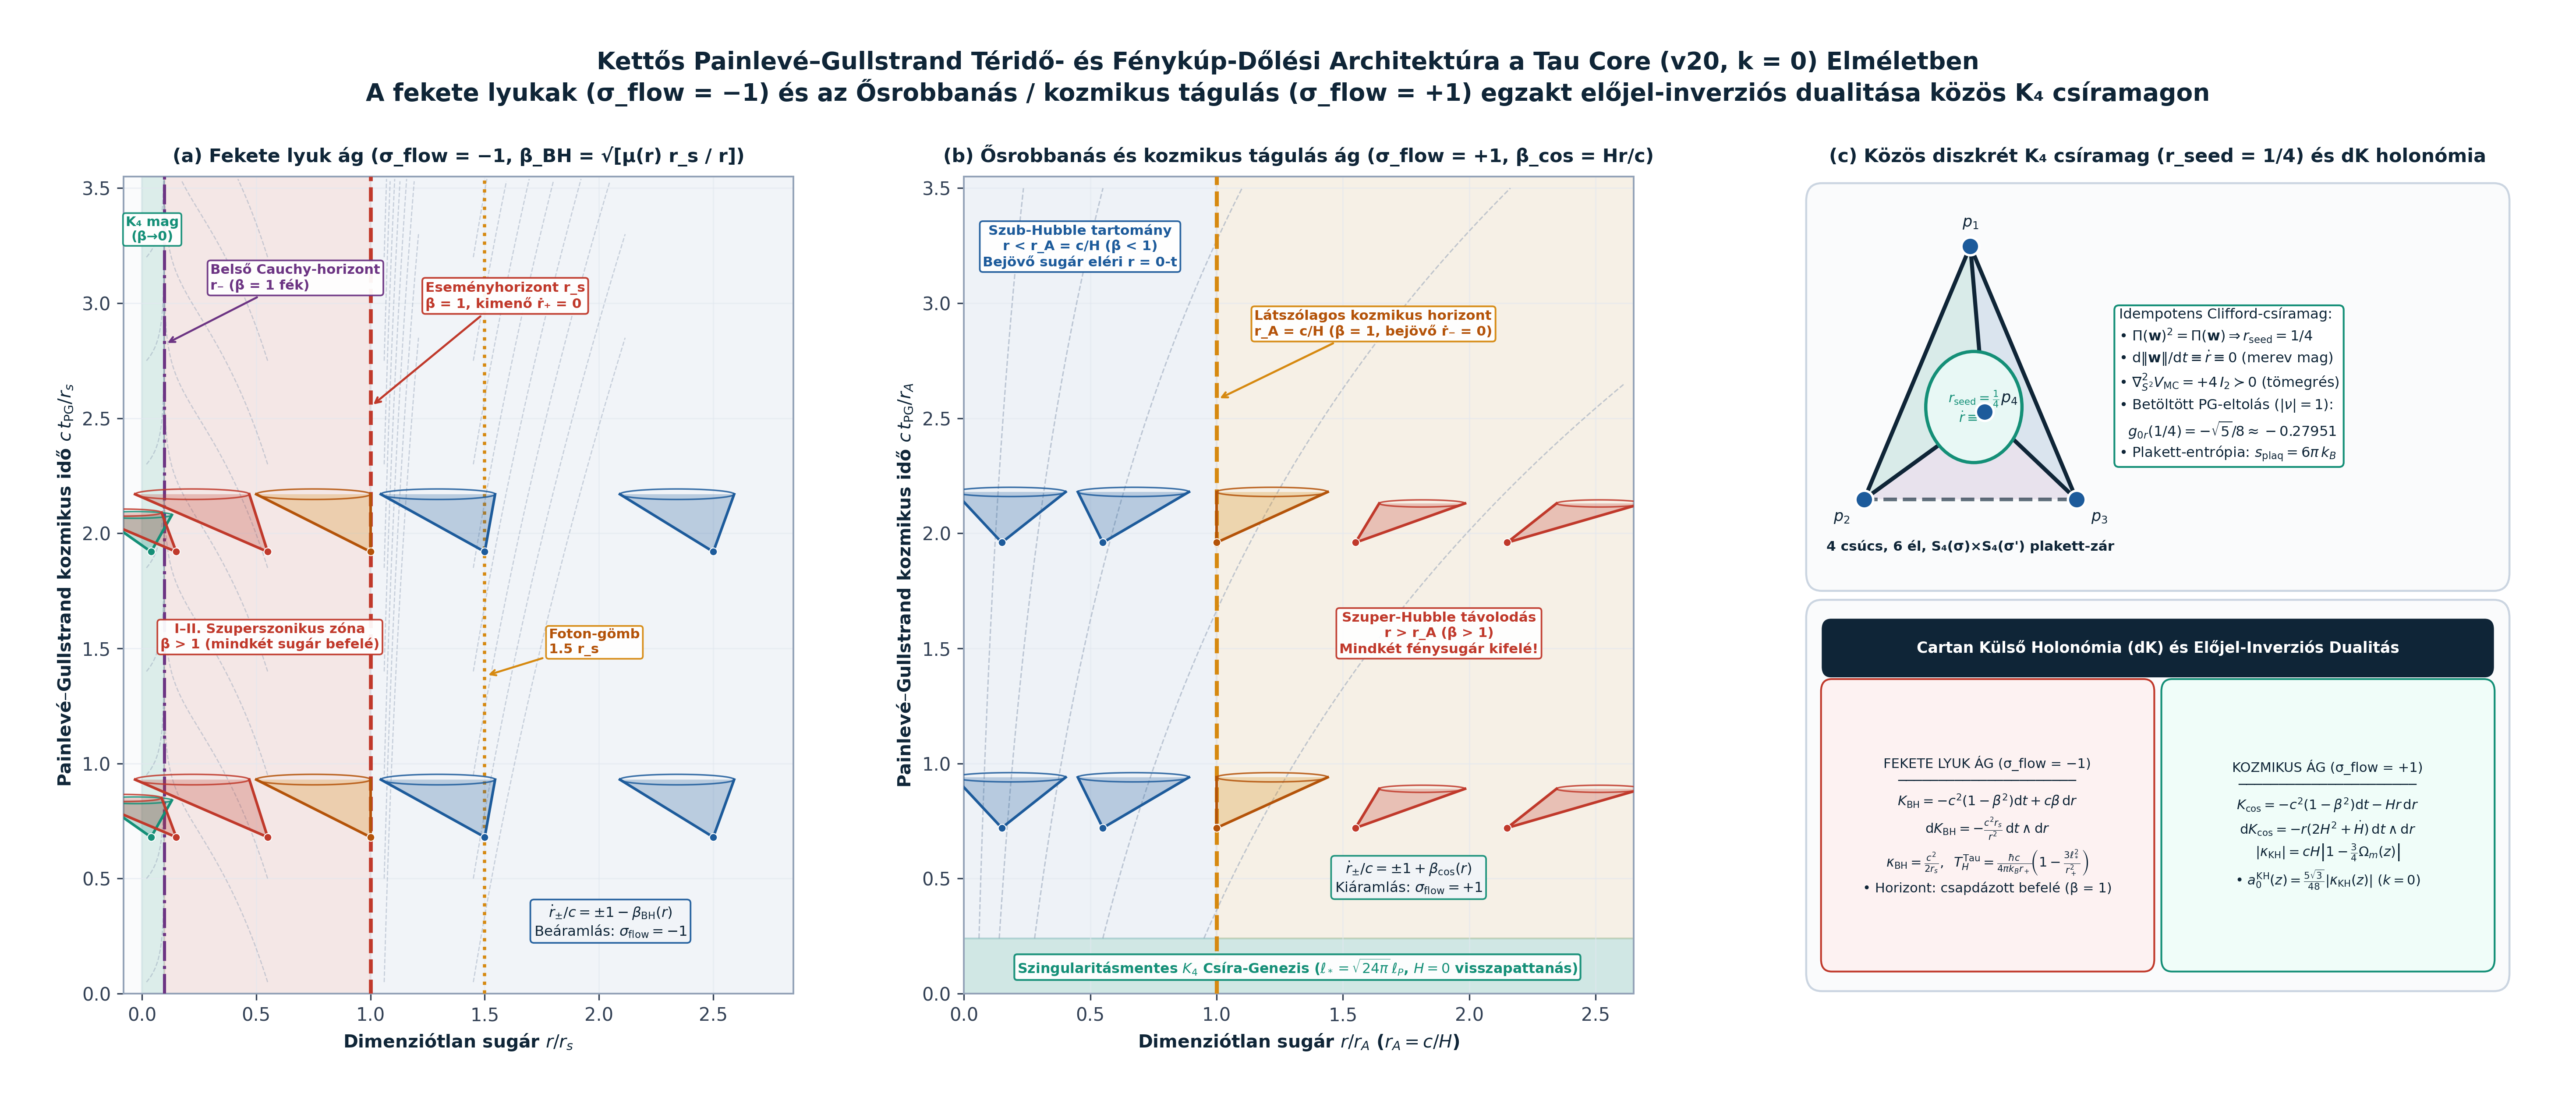
\includegraphics[width=\textwidth]{figures/fig1_pg_duality_and_lightcone_architecture.png}
  \caption{Egyes\'itett Painlev\'e--Gullstrand el\H{o}jel-ford\'it\'asi dualit\'as ($\sigma_{\mathrm{flow}} = -1$ befel\'e zuhan\'o fekete lyuk \'ag kontra $\sigma_{\mathrm{flow}} = +1$ kifel\'e t\'agul\'o kozmol\'ogiai \'ag), radi\'alis f\'enyk\'up-d\H{o}l\'es $\dot{r}_\pm = c(\pm 1 + \sigma_{\mathrm{flow}}\beta)$ a $\beta = 1$ oks\'agi horizontokon \'at, bet\"olt\"ott $K_4$ cs\'ira-eltol\'as $g_{0r}(1/4) = -\sqrt{5}/8 \approx -0.27951$, valamint konnekci\'omentes Cartan $\mathrm{d}K$ k\"uls\H{o} 2-forma holon\'omia (\texttt{D1.\ t\'etel}).}
  \label{fig:fig1_pg_duality}
\end{figure}

Az \ref{fig:fig1_pg_duality}.\ \'abra szeml\'elteti a fekete lyukak horizontj\'at ($\sigma_{\mathrm{flow}} = -1$) \'es a kozmikus l\'atsz\'olagos horizontot ($\sigma_{\mathrm{flow}} = +1$) \"osszek\"ot\H{o} egzakt geometriai t\"uk\"orszimmetri\'at.

% =============================================================================
\section{A szingularit\'asmentes n\'egyz\'on\'as fekete lyuk bels\H{o} anat\'omi\'aja (\texorpdfstring{$\sigma_{\mathrm{flow}} = -1$}{sigma\_flow = -1}, \texttt{D3--D4.\ t\'etelek})}
\label{sec:bh_interior}
% =============================================================================

A klasszikus GR-ben az $r = r_s$ esem\'enyhorizont \'atl\'ep\'ese ut\'an semmi sem \'all\'itja meg az $r = 0$ pontszer\H{u} szingularit\'asig tart\'o \"osszeoml\'ast. A Tau Core ($k = 0$) keret\'eben a diszkr\'et $K_4$ algebra a v\'akuumbels\H{o}t n\'egy koncentrikus, fizikailag elk\"ul\"on\"ul\H{o} kvantumgravit\'aci\'os z\'on\'aval v\'altja fel az $x \equiv r/r_s$ dimenzi\'otlan sug\'ar ment\'en (diagrammatikusan $\epsilon_{\mathrm{core}} = R_{\mathrm{seed}}/r_s = 0.10$, asztrofizikailag pedig $\epsilon_{\mathrm{phys}} = \ell_*/r_s$ felbont\'assal).

\subsection{I.\ Z\'ona (\texorpdfstring{$r_{\mathrm{COCA}} < r < r_s$}{r\_COCA < r < r\_s}): szuperszonikus PG-zuhan\'as \'es \texorpdfstring{$+2:-1:-1$}{+2:-1:-1} \texttt{CHDF} spagettifik\'aci\'o}

K\"ozvetlen\"ul az esem\'enyhorizonton bel\"ul ($x < 1$) a szubsztr\'atum be\'araml\'asa szuperszonikuss\'a (\'es a koordin\'ata-f\'enyk\'uphoz k\'epest szuperlumin\'aliss\'a) v\'alik ($\beta_{\mathrm{Tau}}(r) > 1$), el\'erve a $\beta_{\max} = 2.3151$ cs\'ucs-Mach-sz\'amot a felbontott kvantummag-profilon, miel\H{o}tt a bels\H{o} z\'on\'ak mereved\'ese megkezd\H{o}dne. Mindk\'et radi\'alis f\'enysug\'ar befel\'e mutat ($\dot{r}_+ = c(1 - \beta_{\mathrm{Tau}}) < 0$, $\dot{r}_- = -c(1 + \beta_{\mathrm{Tau}}) < 0$), mik\"ozben a behull\'o anyag saj\'at\'or\'aja zavartalanul $\mathrm{d}\tau_{\mathrm{proper}} = \mathrm{d}t_{\mathrm{PG}}$ \"utemben ketyeg tov\'abb.

Mikrofizikailag a klasszikus Weyl-\'arap\'alyny\'ujt\'as (,,spagettifik\'aci\'o'') k\"ozvetlen\"ul az \eqref{eq:hb_occ_matrix} egyenlet $\mathbf{T}_{\mathrm{def}} \equiv I_4 - H_b^{\mathrm{occ}}$ diszkr\'et \texttt{CHDF} deform\'aci\'os tenzor\'ab\'ol sz\'armazik:
\begin{equation}
  \mathbf{T}_{\mathrm{def}} =
  \begin{pmatrix}
    0 & +\frac{\sqrt{5}}{8} & 0 & 0 \\[4pt]
    +\frac{\sqrt{5}}{8} & +\frac{\sqrt{3}}{12} & 0 & 0 \\[4pt]
    0 & 0 & -\frac{\sqrt{3}}{24} & 0 \\[4pt]
    0 & 0 & 0 & -\frac{\sqrt{3}}{24}
  \end{pmatrix}.
  \label{eq:tdef_matrix}
\end{equation}
A $\mathbf{T}_{\mathrm{def}}$ m\'atrixot az $(\mathbf{e}_r, \mathbf{e}_{t_1}, \mathbf{e}_{t_2})$ $3\times 3$-as t\'erbeli blokkj\'ara megszor\'itva az egzakt saj\'at\'ert\'ekek:
\begin{equation}
  \lambda_r = +\frac{\sqrt{3}}{12} \approx +0.14433757, \qquad
  \lambda_{t_1} = \lambda_{t_2} = -\frac{\sqrt{3}}{24} \approx -0.07216878, \qquad
  \lambda_r + \lambda_{t_1} + \lambda_{t_2} = 0.
  \label{eq:tidal_eigenvalues}
\end{equation}
A t\'erfogatmeg\H{o}rz\H{o}, nyommentes $+2 : -1 : -1$ radi\'alis megny\'ul\'as \'es transzverz\'alis \"osszenyom\'od\'as teh\'at m\'ar a $K_4$ szimplex algebr\'aj\'aba be van k\'odolva, b\'armif\'ele kontinuum g\"orb\"uleti divergencia n\'elk\"ul.

\subsection{II.\ Z\'ona (\texorpdfstring{$r_{\mathrm{Cauchy}} < r < r_{\mathrm{COCA}}$}{r\_Cauchy < r < r\_COCA}): \texttt{COCA-H1} Yukawa-er\H{o}kiolt\'as \'es 48-Weyl dekonfin\'aci\'o}

A newtoni \'es Schwarzschild-gravit\'aci\'oban a $|\nabla\Phi_0| = GM/r^2$ radi\'alis er\H{o} kis t\'avols\'agokon diverg\'al. A $K_4$ teljes gr\'af $L_{K_4} = 4I_4 - \mathbf{1}_4\mathbf{1}_4^T$ Laplace-m\'atrix\'anak spektruma azonban $\{0, 4, 4, 4\}$, ami az \'ora-potenci\'alt egy t\"omegtelen $S_4$-szingulett csatorn\'ara ($-\nabla^2\Phi_0 = 4\pi G\rho$) \'es egy h\'aromzorosan elfajult, t\"omeges $E_3$ triplett csatorn\'ara ($[-\nabla^2 + m_{\mathrm{COCA}}^2]\Phi_m = 4\pi G\rho$) bontja.

\begin{theorem}[\texttt{COCA-H1} $1/r^2$ er\H{o}szingularit\'as-kiolt\'as \'es III--IV.\ z\'onabeli regularit\'as --- \texttt{D3.\ t\'etel}]
\label{thm:d3}
Egy $M$ t\"omeg\H{u} pontforr\'as fizikai $S_4$-szingulett \'ora-potenci\'alja a kivont Yukawa-potenci\'al:
\begin{equation}
  \Phi_{K_4}(r) = \Phi_0(r) - \Phi_m(r) = -\frac{GM}{r}\!\left(1 - e^{-m_{\mathrm{COCA}}\,r}\right), \qquad Z(r) \equiv 1 - e^{-m_{\mathrm{COCA}}\,r}.
  \label{eq:phi_k4_yukawa}
\end{equation}
A $\partial_r\Phi_{K_4}(r)$ radi\'alis \'ora-gradiens er\H{o}t $r = 0$ k\"or\"ul sorba fejtve mind az $1/r^2$, mind az $1/r$ divergensek egzaktul kiesnek, szigor\'uan v\'eges mag-er\H{o}t hagyva vissza:
\begin{equation}
  \frac{\mathrm{d}\Phi_{K_4}}{\mathrm{d}r} = \frac{GM}{r^2}\!\left[1 - \bigl(1 + m_{\mathrm{COCA}}r\bigr)e^{-m_{\mathrm{COCA}}r}\right] = +\frac{1}{2}GM\,m_{\mathrm{COCA}}^2 - \frac{1}{3}GM\,m_{\mathrm{COCA}}^3\,r + \mathcal{O}(r^2).
  \label{eq:coca_finite_force}
\end{equation}
Egyidej\H{u}leg a $G_{K_4}(r) = (1 - e^{-m_{\mathrm{COCA}}r})/(4\pi r)$ Green-f\"uggv\'eny $\partial_i\partial_j G_{K_4}(\mathbf{x})$ disztrib\'uci\'os Hesse-m\'atrix\'aban a $\Phi_0$-b\'ol sz\'armaz\'o $-\frac{1}{3}\delta_{ij}\delta^{(3)}(\mathbf{x})$ Dirac-delta kontakt-szingularit\'ast egzaktul kiejti $\Phi_m$ azonos kontakt-tagja.
\end{theorem}

\begin{proof}
Az $e^{-m_{\mathrm{COCA}}r} = 1 - m_{\mathrm{COCA}}r + \frac{1}{2}m_{\mathrm{COCA}}^2 r^2 - \frac{1}{6}m_{\mathrm{COCA}}^3 r^3 + \mathcal{O}(r^4)$ Taylor-sort az $(1 + m_{\mathrm{COCA}}r)e^{-m_{\mathrm{COCA}}r}$ szorzatba helyettes\'itve $1 - \frac{1}{2}m_{\mathrm{COCA}}^2 r^2 + \frac{1}{3}m_{\mathrm{COCA}}^3 r^3 + \mathcal{O}(r^4)$ ad\'odik. Az $1 - (1 + m_{\mathrm{COCA}}r)e^{-m_{\mathrm{COCA}}r}$ k\"ul\"onbs\'eget $r^2$-tel osztva az $r^{-2}$ \'es $r^{-1}$ tagok marad\'ektalanul kiesnek, megadva az \eqref{eq:coca_finite_force} egyenletet (\texttt{SymPy} \'altal ellen\H{o}rizve). Mivel $-\nabla^2 G_0 = \delta^{(3)}(\mathbf{x})$ \'es $(-\nabla^2 + m_{\mathrm{COCA}}^2)G_m = \delta^{(3)}(\mathbf{x})$, k\"ul\"onbs\'eg\"uk $-\nabla^2 G_{K_4} = -m_{\mathrm{COCA}}^2 G_m \in L^1_{\mathrm{loc}}(\mathbb{R}^3)$, ami elt\"unteti a $\delta^{(3)}(\mathbf{x})$ kontakt-szingularit\'ast. L\'enyeges geometriai k\"ul\"onbs\'eg, hogy m\'ig a pontszer\H{u} Yukawa-potenci\'al k\"ozvetlen $f_{\mathrm{naive}}(r) = 1 - \frac{r_s}{r}(1 - e^{-m_{\mathrm{COCA}}r})$ behelyettes\'it\'ese $f'_{\mathrm{naive}}(0) \neq 0$ k\'up-szingularit\'ast \'es divergens $R_{\mathrm{naive}}(r) = \frac{2m_{\mathrm{COCA}}r_s}{r^2} - \frac{3m_{\mathrm{COCA}}^2 r_s}{r} + \mathcal{O}(1)$ Ricci-g\"orb\"uletet hagyna vissza, a fizikai 3D Painlev\'e--Gullstrand $\mathbf{v}(\mathbf{x}) = -c\beta_{\mathrm{Tau}}(r)\mathbf{x}/r$ sebess\'egvektor $C^\infty(\mathbb{R}^3)$ simas\'aga $\mathbf{x} = \mathbf{0}$-ban (amelyet a v\'eges $R_{\mathrm{seed}} \sim \ell_*$ IV.\ z\'onabeli projektormag k\'enyszer\'it ki) p\'aratlan radi\'alis parit\'ast ($\beta_{\mathrm{Tau}}(r) = r/\ell_* + \mathcal{O}(r^3)$), $f'_{\mathrm{eff}}(0) = 0$ felt\'etelt \'es szigor\'uan v\'eges $R_{\mathrm{Tau}}(0) = 12/\ell_*^2$ k\"ozponti Ricci-skal\'art biztos\'it (\texttt{SymPy} \'altal igazolva).
\end{proof}

Ahogy a behull\'o barionos \'es leptonos anyag \'athalad a II.\ z\'on\'an \'es a lok\'alis \'arap\'aly-/kompresszi\'os energia meghaladja a QCD ($\sim 0.2\;\mathrm{GeV}$), majd az elektrogyenge ($\sim 246\;\mathrm{GeV}$) k\"usz\"ob\"ot, az \"osszetett hadronok \'es t\"omeges SM \'iz-saj\'at\'allapotok \textbf{szimplici\'alis dekonfin\'aci\'on} mennek kereszt\"ul (\texttt{VII-A.\ \'es 15.\ tanulm\'any}) \cite{JolcsakTauFoundationSeries2026}: a h\'arom kir\'alis fermion-gener\'aci\'o ($3 \times 16 = 48$ Weyl-spinor szabads\'agi fok) visszaolvad az $\mathcal{A}_4 \otimes \mathrm{Cl}(V_3)$ algebr\'an \'el\H{o} s\'ertetlen, t\"omegtelen szimmetrikus f\'azisba. A barion- \'es leptonsz\'amok nem semmis\"ulnek meg szingularit\'asban, hanem a szimplici\'alis kondenz\'atum topologikus t\"olt\'eseik\'ent maradnak meg.

\subsection{III.\ Z\'ona (\texorpdfstring{$R_{\mathrm{seed}} < r < r_{\mathrm{Cauchy}}$}{R\_seed < r < r\_Cauchy}): 15-csatorn\'as \texttt{CHDF}-f\'ek \'es \texorpdfstring{$\pi_2(S^2) = \mathbb{Z}$}{pi\_2(S\^2) = Z} spin-text\'ura}

Klasszikus Kerr- vagy Reissner--Nordstr\"om-bels\H{o}kben az $r_-$ bels\H{o} Cauchy-horizont fel\'e tart\'o hull\'amok v\'egtelen k\'ekeltol\'od\'ast szenvednek, ami exponenci\'alis Poisson--Israel t\"omeginfl\'aci\'ot v\'alt ki \cite{PoissonIsrael1990}. A Tau Core-ban a III.\ z\'ona k\'et egzakt mechanizmussal stabiliz\'alja a bels\H{o} \'atmenetet:
\begin{enumerate}
  \item \textbf{15-csatorn\'as \texttt{CHDF} UV-nyomkiolt\'as:} A $K_4$ szimplex 15-dimenzi\'os skal\'ar fluktu\'aci\'os multiplettj\'en a csatornas\'ulyok z\'er\'o ered\H{o} nyommal p\'arosodnak ki:
  \begin{align}
    \mathrm{Tr}\!\bigl(T_{\mathrm{def}}^{(15)}\bigr)
    &= 3\cdot\!\left(+\frac{1}{3}\right) + 3\cdot\!\left(-\frac{1}{3}\right) + 9\cdot 0 = 0 \nonumber\\
    &\Longleftrightarrow\;
    \frac{\sqrt{3}}{24}\bigl[1(+5)_{\mathbf{1}} + 3(-1)_{\mathbf{3}} + 2(-1)_{\mathbf{2}} + 3(+1)_{\mathbf{3}'} + 6(-1/2)_{\mathbf{6}}\bigr] = 0.
    \label{eq:chdf_15_trace}
  \end{align}
  A Frullani-f\'ele integr\'alazonoss\'aggal kombin\'alva (\ref{sec:big_bang}.\ szakasz) az \eqref{eq:chdf_15_trace} egyenlet kioltja az \"osszes kvadratikus \'es logaritmikus UV-divergenci\'at eg\'eszen $M_* = E_P/\sqrt{24\pi}$-ig, a k\'ekeltol\'odott energiafelhalmoz\'od\'ast egy merev akusztikus f\'ekez\H{o}r\'etegg\'e ($w_{\mathrm{eff}} \to +1$, majd sima \'atmenet $-1$ fel\'e) tel\'itve, amely $\beta_{\mathrm{Tau}}(x)$-et $1$ al\'a lass\'itja vissza a regul\'aris bels\H{o} Cauchy-horizonton ($x_- = 0.032311$ az $\epsilon_{\mathrm{core}} = 0.10$ profilon).
  \item \textbf{Topologikus $\pi_2(S^2) = \mathbb{Z}$ perd\"ulett\'arol\'as:} Forg\'o fekete lyukra ($J = aMc$) a klasszikus GR szingul\'aris egyenl\'it\H{o}i gy\H{u}r\H{u}t ($r = 0, \theta = \pi/2$) \'es oks\'ags\'ert\H{o} z\'art id\H{o}szer\H{u} g\"orb\'eket (CTC) j\'osol. Mivel azonban a $K_4$ direktor-mez\H{o} ($\hat{\mathbf{u}}_\sigma \in S^2$) kiel\'eg\'iti a $\pi_0(S^2) = 0$, $\pi_1(S^2) = 0$ (nincs szingul\'aris \"orv\'enyvonal) \'es $\pi_2(S^2) = \mathbb{Z}$ homot\'opi\'at (v\'eges Dirichlet-energi\'aj\'u Skyrme/s\"un-text\'ur\'ak: $\int |\nabla\hat{\mathbf{u}}|^2\,\mathrm{d}^3x = 8\pi R_{\mathrm{core}} < \infty$), a perd\"ulet kvant\'alt $\pi_2(S^2) = \mathbb{Z}$ spinor-kondenz\'atum \"orv\'enyess\'egbe ker\"ul, meg\H{o}rizve a glob\'alis PG-id\H{o}ir\'anyt ($\mathrm{d}t_{\mathrm{PG}} > 0$, nulla CTC).
\end{enumerate}

\subsection{IV.\ Z\'ona (\texorpdfstring{$r \le R_{\mathrm{seed}}$}{r <= R\_seed}): inkompresszibilis \texorpdfstring{$K_4$}{K4} kvantum-cs\'iramag (\texttt{D4.\ t\'etel})}

\begin{theorem}[Algebrai projektor-szuperszelekci\'o \'es univerz\'alis g\"orb\"uleti plafon --- \texttt{D4.\ t\'etel}]
\label{thm:d4}
A $\mathrm{Cl}(V_3) \cong M_2(\mathbb{C})$ Clifford-spinor algebr\'aban legyen $\Pi(\mathbf{w}) = \frac{1}{2}(I_2 + 2\mathbf{w}\cdot\boldsymbol{\sigma})$, ahol $\|\mathbf{w}\|_2 = r$. Ekkor:
\begin{enumerate}
  \item Az 1-rang\'u projektor idempotenci\'aja, $\Pi(\mathbf{w})^2 - \Pi(\mathbf{w}) = (r^2 - \frac{1}{4})I_2 = 0$, egy\'ertelm\H{u}en kik\'enyszer\'iti az $r = r_{\mathrm{seed}} = 1/4$ norm\'at, tetsz\H{o}leges sima $\mathbf{w}(t)$ p\'alya menti deriv\'al\'asa pedig $2(\mathbf{w}\cdot\dot{\mathbf{w}})I_2 = 0 \implies \dot{r} \equiv 0$ k\'enyszert ad, els\H{o} rendben tiltva az $r \to 0$ ir\'any\'u radi\'alis \"osszenyom\'ast.
  \item Az $S^2$ egys\'egg\"omb\"on a kir\'alis tetra\'eder-cs\'ucsok ($\nu\mathbf{v}_{\mathrm{root}} = \frac{\nu}{\sqrt{3}}(1,1,1)$, $\nu = \pm 1$) k\"or\"uli sz\"ogdeform\'aci\'okat pozit\'iv definit Maurer--Cartan Hesse-m\'atrix v\'edi: $\nabla^2_{S^2} V_{\mathrm{MC}}\big|_{\nu\mathbf{v}_{\mathrm{root}}} = 4I_2 \succ 0$, $\Delta V_{\mathrm{MC}}/r_{\mathrm{seed}}^4 = 1/2$ okta\'ederes g\'attal.
  \item K\"ovetkez\'esk\'eppen az $r \le R_{\mathrm{seed}}$ k\"ozponti mag inkompresszibilis, regul\'aris de Sitter-f\'azist alkot $\beta_{\mathrm{Tau}}(0) = 0$, $f_{\mathrm{eff}}(0) = +1$, $w(0) = p_r/\rho = -1$ v\'akuum \'allapotegyenlettel \'es a fekete lyuk $M$ t\"omeg\'et\H{o}l f\"uggetlen univerz\'alis Planck-sk\'al\'as Kretschmann-g\"orb\"uleti korl\'attal:
  \begin{equation}
    \mathcal{K}_{\mathrm{Tau}}(r) \xrightarrow{r \to 0} \mathcal{K}_{\max} \le \frac{24}{\ell_*^4} = \frac{24}{(24\pi\,\ell_P^2)^2} = \frac{1}{24\pi^2\,\ell_P^4} \approx \frac{4.2217 \times 10^{-3}}{\ell_P^4} < \infty.
    \label{eq:kretschmann_bound}
  \end{equation}
\end{enumerate}
\end{theorem}

\begin{proof}
A $\Pi(\mathbf{w})^2 = \frac{1}{4}(I_2 + 4\mathbf{w}\cdot\boldsymbol{\sigma} + 4\|\mathbf{w}\|_2^2 I_2)$ kifejt\'es a $(\mathbf{w}\cdot\boldsymbol{\sigma})^2 = \|\mathbf{w}\|_2^2 I_2$ azonoss\'aggal $\Pi^2 - \Pi = (r^2 - 1/4)I_2 = 0 \iff r = 1/4$ eredm\'enyt ad, amelynek id\H{o}deriv\'altja $2r\dot{r} = 0 \implies \dot{r} \equiv 0$. A $V_{\mathrm{MC}}(\mathbf{u}) = 1 + 2\sqrt{3}u_1 u_2 u_3 + \frac{1}{2}\|\mathbf{u}\|_2^4 - \frac{3}{2}(u_1^4+u_2^4+u_3^4)$ potenci\'al \'erint\H{o} Hesse-m\'atrixa $\|\mathbf{u}\|_2 = 1$ mellett $\nu\mathbf{v}_{\mathrm{root}}$-ban $\mathrm{diag}(4, 4) \succ 0$ \cite{JolcsakTauFoundationSeries2026}. Hayward-regulariz\'alt de Sitter magra ($f_{\mathrm{eff}}(r) = 1 - r_s r^2/(r^3 + r_s \ell_*^2) \simeq 1 - r^2/\ell_*^2$, $r \to 0$) a k\"ozponti Kretschmann-skal\'ar $\mathcal{K}(0) = 24/\ell_*^4$; behelyettes\'itve $\ell_*^2 = 24\pi\ell_P^2$-t, $\mathcal{K}_{\max}\ell_P^4 = 24/(576\pi^2) = 1/(24\pi^2) \approx 4.221716 \times 10^{-3}$ ad\'odik.
\end{proof}

A \ref{tab:bh_zones}.\ t\'abl\'azat \"osszegzi a radi\'alis z\'ona-anat\'omi\'at a k\"uls\H{o} akkr\'eci\'os korongt\'ol ($x = 3$) a k\"ozponti $K_4$ cs\'iramagig ($x \to 0$), a \ref{fig:fig2_bh_anatomy}.\ \'abra pedig a folytonos radi\'alis profilokat mutatja be.

\begin{table}[htbp]
\centering
\caption{A fekete lyuk koncentrikus radi\'alis anat\'omi\'aja a Tau Core elm\'eletben ($\sigma_{\mathrm{flow}} = -1$, $k = 0$), \"osszevetve a klasszikus Schwarzschild/Kerr GR-rel az $x = r/r_s$ sug\'ar ment\'en ($\epsilon_{\mathrm{core}} = 0.10$ felbontott bels\H{o}-z\'ona sk\'al\'aval).}
\label{tab:bh_zones}
\vspace{4pt}
\resizebox{\textwidth}{!}{%
\footnotesize
\begin{tabular}{L{2.5cm}L{3.3cm}C{1.9cm}C{1.8cm}C{1.6cm}L{2.8cm}L{3.7cm}}
\toprule
\textbf{Sug\'ar $x=r/r_s$} & \textbf{Fizikai z\'ona} & \textbf{PG-sebess\'eg $\beta_{\mathrm{Tau}}$} & \textbf{Metrika $f_{\mathrm{eff}}$} & \textbf{EoS $w_{\mathrm{eff}}$} & \textbf{Kretschmann $\mathcal{K}$ (GR vs.\ Tau)} & \textbf{Domin\'ans mikrofizika ($k = 0$)} \\
\midrule
$x \ge 1.50$ & Foton-g\"omb \'es ISCO ($x=3$) & $\le 0.8165$ & $\ge +0.333$ & $0$ & GR $\equiv$ Tau ($<10^{-27}$ elt\'er\'es) & V\'akuum PG-be\'araml\'as; EHT foton-gy\H{u}r\H{u} \'ep \\
$x = 1.00$ & K\"uls\H{o} esem\'enyhorizont $\partial\mathcal{M}_H$ & $1.0000$ & $0.000$ & $0$ & V\'eges: $12/r_s^4$ & $\dot{r}_+ = 0$; $S_{\mathrm{BH}}/k_B = 6\pi(A_H/\ell_*^2)$ felszabadul \\
$0.48 < x < 1.00$ & \textbf{I.\ Z\'ona:} Szuperszonikus PG-zuhan\'as & $1.00 \to 1.56$ & $< 0$ & $\simeq +1/3$ & Sim\'an a GR alatt korl\'atos & $\mathbf{T}_{\mathrm{def}}$ $(\frac{\sqrt{3}}{12}, -\frac{\sqrt{3}}{24}, -\frac{\sqrt{3}}{24})$ $+2:-1:-1$ \'arap\'aly \\
$0.22 < x \le 0.48$ & \textbf{II.\ Z\'ona:} \texttt{COCA-H1} \'es dekonfin\'aci\'o & $1.56 \to 2.13$ & $< 0$ & $+1/3 \to +1$ & $1/r^2$ \'es $\delta^{(3)}$ kioltva & $\Phi_{K_4}=\Phi_0-\Phi_m$ mag-er\H{o} $+\frac{1}{2}GMm_{\mathrm{COCA}}^2$; 48-Weyl olvad\'as \\
$0.0323 < x \le 0.22$ & \textbf{III.\ Z\'ona:} \texttt{CHDF} UV-f\'ek & Cs\'ucs $2.315 \to 1$ & $< 0 \to 0$ & $+1 \to -0.98$ & T\"omeginfl\'aci\'o meg\'all\'itva & $\mathrm{Tr}(T_{\mathrm{def}}^{(15)})=0$ UV-lev\'ag\'as; $\pi_2(S^2)=\mathbb{Z}$ spin-text\'ura \\
$0 \le x \le 0.0323$ & \textbf{IV.\ Z\'ona:} $K_4$ kvantum-cs\'iramag & $1.00 \to 0.00$ & $0 \to +1.00$ & $-1.000$ & \textbf{GR: $\infty$} vs.\ \textbf{Tau: $\frac{1}{24\pi^2\ell_P^4}$} & $\Pi^2=\Pi \implies r_{\mathrm{seed}}=1/4, \dot{r}=0$; $\nabla^2_{S^2}V_{\mathrm{MC}}=4I_2\succ 0$ \\
\bottomrule
\end{tabular}%
}
\end{table}

\begin{figure}[htbp]
  \centering
  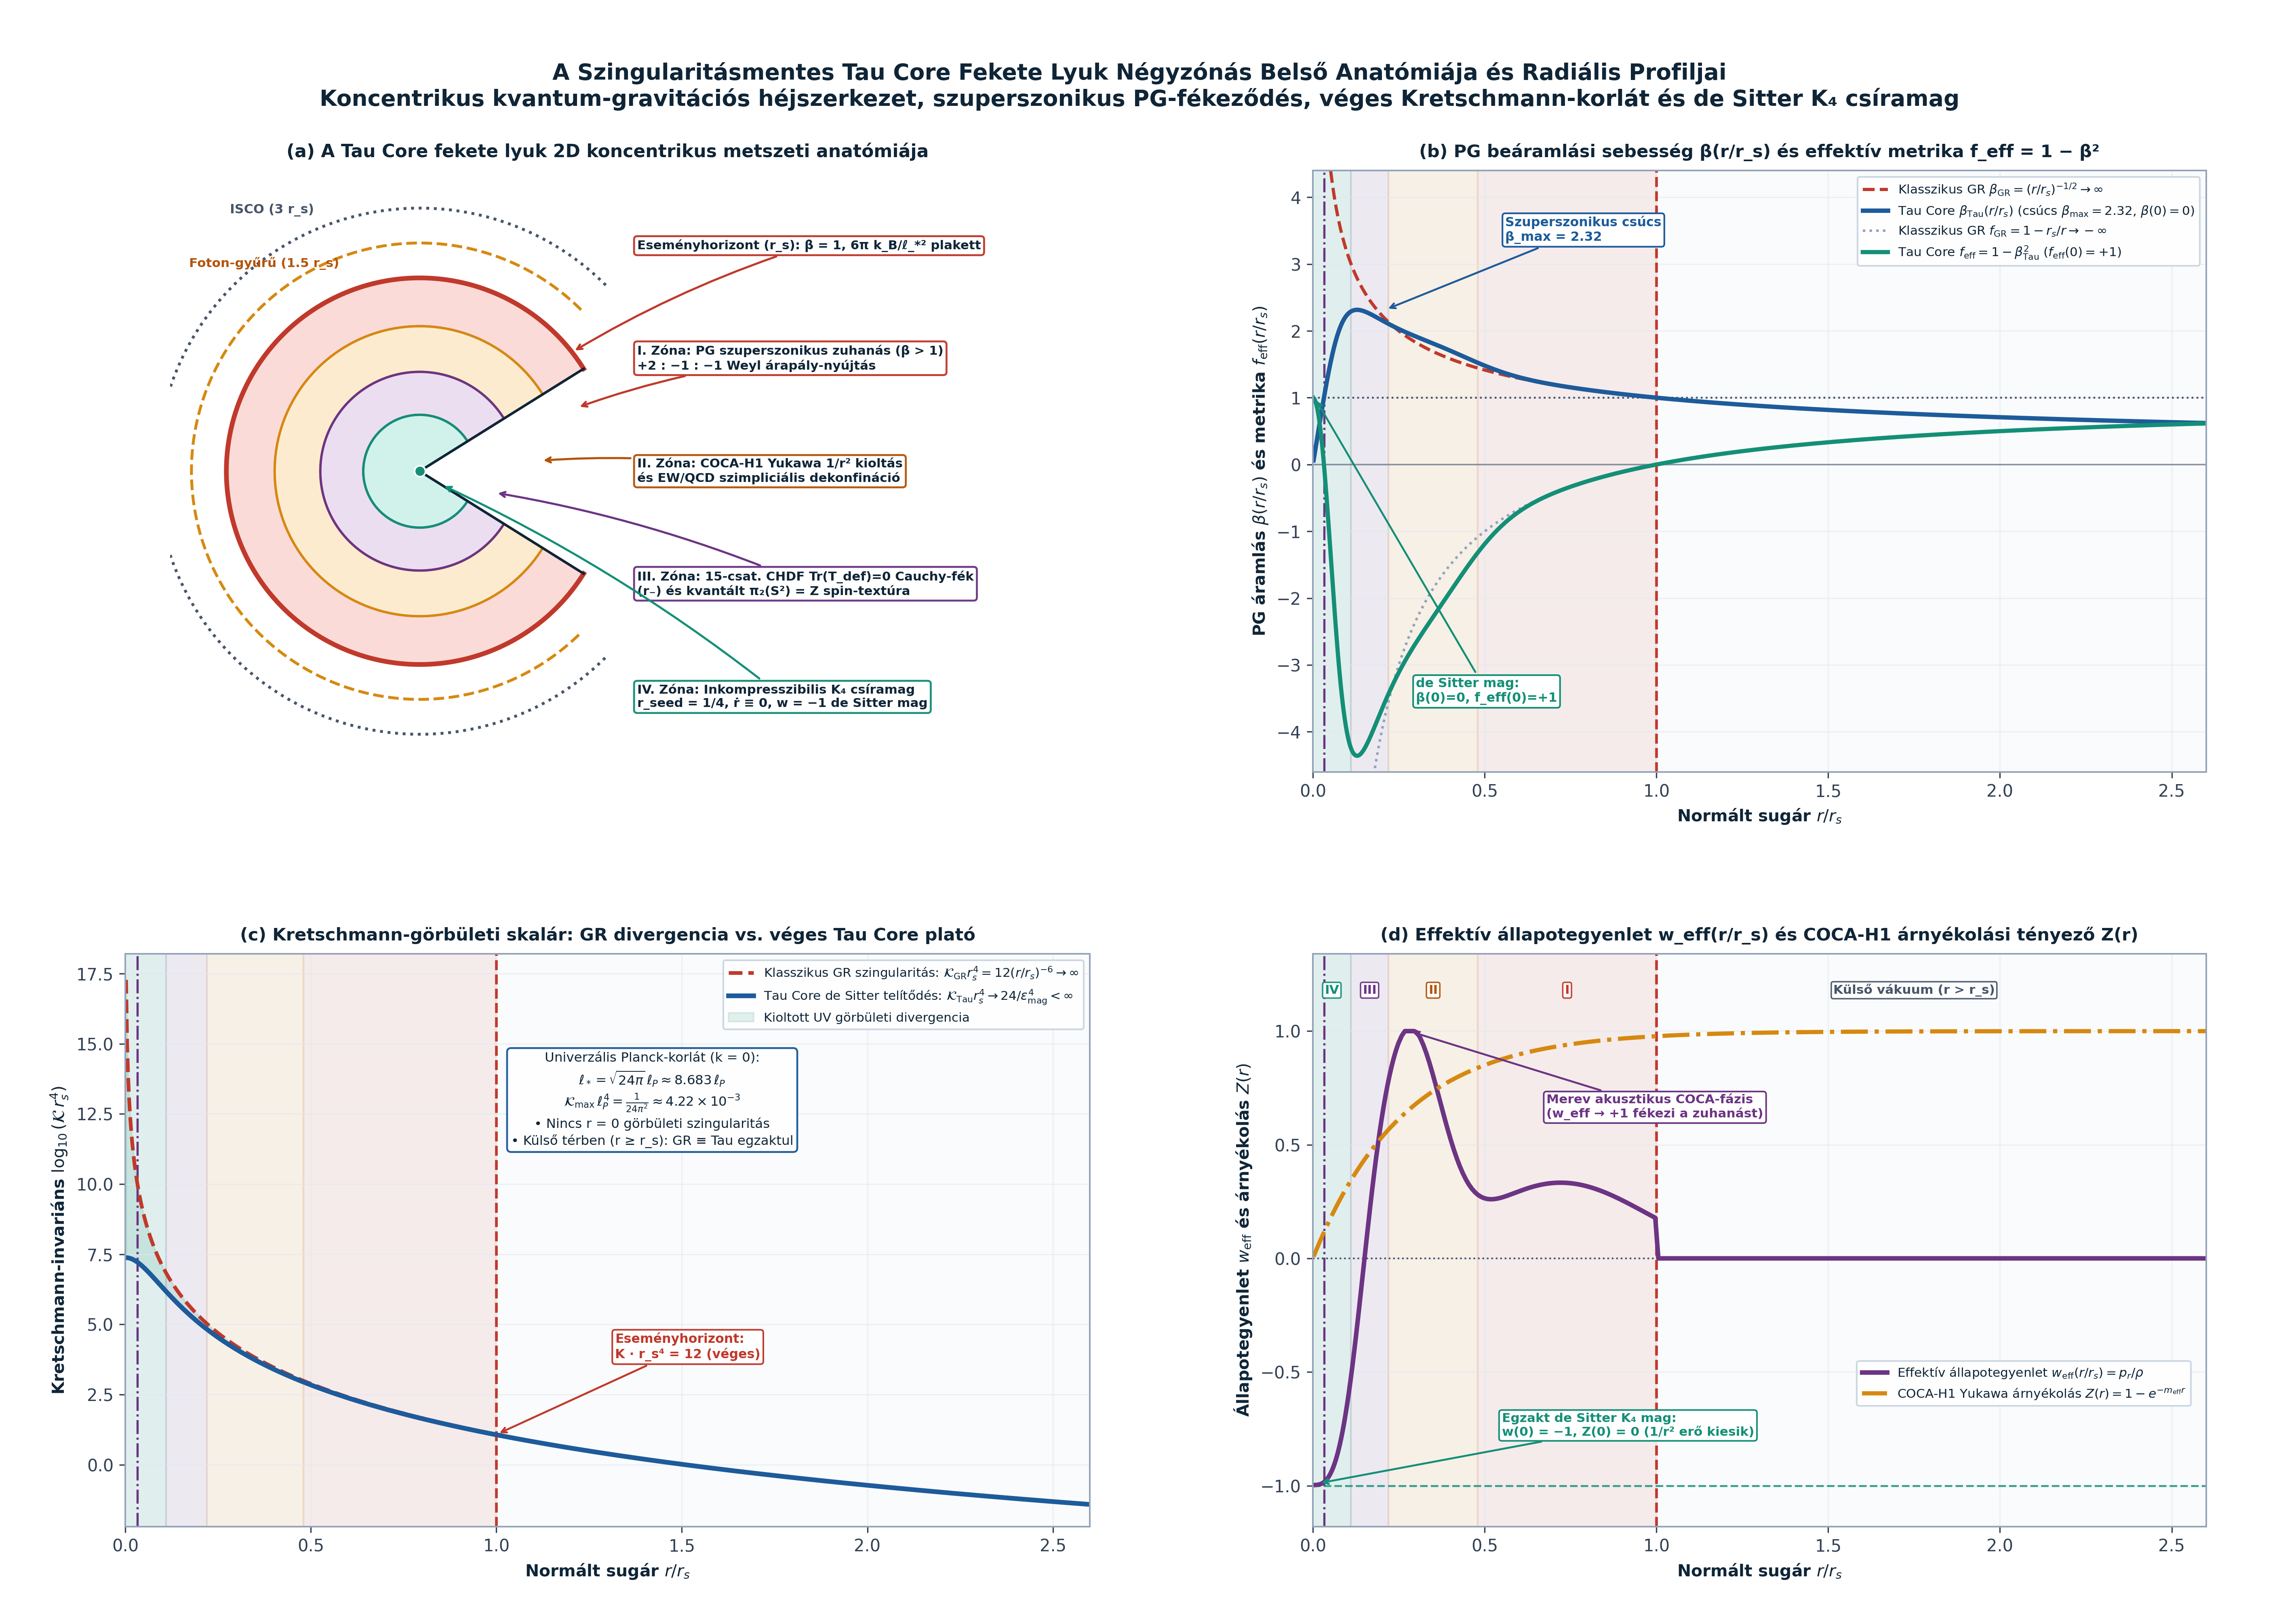
\includegraphics[width=\textwidth]{figures/fig2_black_hole_four_zone_interior_anatomy.png}
  \caption{A fekete lyuk szingularit\'asmentes n\'egyz\'on\'as bels\H{o} anat\'omi\'aja ($\sigma_{\mathrm{flow}} = -1$, \texttt{D3--D4.\ t\'etelek}): radi\'alis PG-be\'araml\'asi sebess\'eg $\beta_{\mathrm{Tau}}(x)$ a divergens GR $\beta_{\mathrm{GR}} = x^{-1/2}$ g\"orb\'evel szemben, az $f_{\mathrm{eff}}(x) = 1 - \beta_{\mathrm{Tau}}^2$ effekt\'iv metrika \'athalad\'asa az $x_- \approx 0.0323$ regul\'aris bels\H{o} Cauchy-horizonton az $f_{\mathrm{eff}}(0) = +1$ de Sitter magig, a korl\'atos $\mathcal{K}_{\mathrm{Tau}}$ Kretschmann-skal\'ar a $12/x^6$ szingularit\'assal szemben, valamint az \'allapotegyenlet alakul\'asa az inkompresszibilis $w(0) = -1$ $K_4$ cs\'iramagig.}
  \label{fig:fig2_bh_anatomy}
\end{figure}

% =============================================================================
\section{Szingularit\'asmentes \texorpdfstring{$K_4$}{K4} Cs\'ira-Genezis (,,Nagy Bumm'' visszapattan\'as), v\'akuumkiolt\'as \'es a gyorsul\'as--dip koincidencia (\texttt{D2.\ t\'etel})}
\label{sec:big_bang}
% =============================================================================

\subsection{Szingularit\'asmentes \texorpdfstring{$K_4$}{K4} Cs\'ira-Genezis visszapattan\'as \texorpdfstring{$\ell_* = \sqrt{24\pi}\,\ell_P$}{ell\_* = sqrt(24 pi) ell\_P} sk\'al\'an}

A PG-\'araml\'asi parit\'as $\sigma_{\mathrm{flow}} = -1 \to +1$ megford\'it\'asa az inkompresszibilis IV.\ z\'onabeli fekete lyuk magot k\"ozvetlen\"ul az Univerzum legkor\'abbi korszak\'ara k\'epezi le. A klasszikus FLRW-kozmol\'ogi\'aban a sug\'arz\'asdomin\'alt $H_{\mathrm{std}}(a) = H_0\sqrt{\Omega_{r,0}\,a^{-4} + \Omega_{m,0}\,a^{-3} + \Omega_{\Lambda,0}}$ r\'at\'at $a \to 0$ fel\'e visszafel\'e extrapol\'alva az $r_A = c/H_{\mathrm{std}}(a)$ l\'atsz\'olagos kozmikus horizont az $\ell_* = \sqrt{24\pi}\,\ell_P = 1.403429 \times 10^{-34}\;\mathrm{m}$ elemi szimplici\'alis r\'acshossz al\'a zsugorodna.

Mivel a $K_4$ projektor-szuperszelekci\'os t\"orv\'eny ($\Pi^2 = \Pi \implies r_{\mathrm{seed}} = 1/4, \dot{r} \equiv 0$, \texttt{D4.\ t\'etel}) a k\"uls\H{o} spinortranszportot a kompakt $\mathrm{SU}(2) \subset \mathrm{Cl}(V_3)$ spincsoportba \'agyazza az $\ell_*^2 = 24\pi\,\ell_P^2$ elemi plaketteken, az $\{a, p_a\} = 1$ ($p_a = -\frac{3c^2}{4\pi G}a\dot{a}$) ADM kanonikus konjug\'alt p\'ar a kompakt $\theta = -\frac{4\pi G\ell_*}{3c^3 a^2}p_a$ holon\'omiasz\"og\"on kereszt\"ul l\'ep be a $\mathcal{C}_{\mathrm{hol}}(a, p_a) = -\frac{3c^4}{8\pi G\ell_*^2}a^3\sin^2\theta + a^3\rho c^2 = 0$ Wilson--Regge Hamilton-k\'enyszerbe. A $\frac{\dot{a}}{a} = \frac{1}{a}\frac{\partial\mathcal{C}_{\mathrm{hol}}}{\partial p_a} = \frac{c}{\ell_*}\sin|\theta|\cos|\theta|$ Hamilton-egyenlet \'es a $\sin^2\theta = H_{\mathrm{std}}^2 / (c/\ell_*)^2$ k\'enyszer szabad param\'eterek n\'elk\"ul ($k = 0$) azonosan megadja a korai Univerzum visszapattan\'asi Friedmann-t\"orv\'eny\'et:
\begin{equation}
  H^2(a) = H_{\mathrm{std}}^2(a)\!\left[1 - \left(\frac{H_{\mathrm{std}}(a)}{H_{\mathrm{crit}}}\right)^2\right], \qquad H_{\mathrm{crit}} = \frac{c}{\ell_*} = \frac{c}{\sqrt{24\pi}\,\ell_P} = 2.136143 \times 10^{42}\;\mathrm{s}^{-1}.
  \label{eq:bounce_friedmann}
\end{equation}
Az \eqref{eq:bounce_friedmann} egyenletb\H{o}l a korai Univerzum h\'arom egzakt genezis-jellemz\H{o}je ad\'odik (\texttt{paper21\_\allowbreak bh\_\allowbreak cosmology\_\allowbreak duality\_\allowbreak results.json}):
\begin{enumerate}
  \item \textbf{Sima, szingularit\'asmentes visszafordul\'as ($H = 0$):} Az $a = 0$-beli divergencia helyett $H(a)$ sim\'an elt\H{u}nik, amikor $H_{\mathrm{std}}(a_{\mathrm{bounce}}) = H_{\mathrm{crit}}$, ami a sug\'arz\'asdomin\'alt korszakban ($H_{\mathrm{std}} \simeq H_0\sqrt{\Omega_{r,0}}\,a^{-2}$) az al\'abbi sk\'alafaktorn\'al k\"ovetkezik be:
  \begin{equation}
    a_{\mathrm{bounce}} = \sqrt{\frac{H_0\sqrt{\Omega_{r,0}}}{c/\ell_*}} = 9.887031 \times 10^{-32}, \qquad \log_{10} a_{\mathrm{bounce}} = -31.00493 \approx -31.005.
    \label{eq:a_bounce}
  \end{equation}
  \item \textbf{Maxim\'alis visszapattan\'as ut\'ani Hubble-r\'ata:} Az \eqref{eq:bounce_friedmann} kifejez\'es $H_{\mathrm{std}}^2$ szerinti maximuma $H_{\mathrm{std}}^2 = \frac{1}{2}H_{\mathrm{crit}}^2$ ($a = 2^{1/4}a_{\mathrm{bounce}}$) eset\'en \'all el\H{o}, megadva az univerz\'alis maxim\'alis kozmikus t\'agul\'asi sebess\'eget:
  \begin{equation}
    H_{\max} = \frac{H_{\mathrm{crit}}}{2} = \frac{c}{2\ell_*} = 1.068071 \times 10^{42}\;\mathrm{s}^{-1} \quad \bigl(\log_{10}[H_{\max}/\mathrm{s}^{-1}] = 42.0286\bigr),
    \label{eq:h_max_bounce}
  \end{equation}
  ami $r_{A,\min} = c/H_{\max} = 2\ell_*$ minim\'alis l\'atsz\'olagos kozmikus horizontsug\'arnak felel meg.
  \item \textbf{De Sitter Cs\'ira-Genezis \'allapotegyenlet:} $a \to a_{\mathrm{bounce}}^+$ k\"ozel\'eben az effekt\'iv $q_{\mathrm{Tau}}(a)$ lassul\'asi param\'eter \'es a $w_{\mathrm{cos}}(a) = (2q_{\mathrm{Tau}} - 1)/3$ kozmikus \'allapotegyenlet sim\'an $q_{\mathrm{Tau}} \to -1$ \'es $w_{\mathrm{cos}} \to -1$ \'ert\'ekhez tart, miel\H{o}tt \'atvezetne a standard sug\'arz\'as- ($w_{\mathrm{cos}} = +1/3$, $q = +1$), anyag- ($w_{\mathrm{cos}} = 0$, $q = +1/2$) \'es k\'es\H{o}i gyorsul\'o korszakba ($q_0 = -0.5271$).
\end{enumerate}

\subsection{60 nagys\'agrend\H{u} UV v\'akuumenergia-kiolt\'as a \texttt{CHDF} \'es Frullani-RG r\'ev\'en}

Mi\'ert nem gravit\'al a $K_4$ szubsztr\'atum $M_* = E_P/\sqrt{24\pi} = 1.4060 \times 10^{18}\;\mathrm{GeV}$ Planck-sk\'al\'aj\'u energi\'aja $\rho_{\mathrm{vac}} \sim M_*^4 \sim 10^{120}\rho_{\Lambda,\mathrm{obs}}$ kozmol\'ogiai \'alland\'ok\'ent? A \texttt{III.\ Pill\'er} (\texttt{F3.\ t\'etel}) \cite{JolcsakTauFoundationSeries2026} k\'et egzakt kvantumt\'erelm\'eleti azonoss\'aga v\'edi az infrav\"or\"os kozmoszt $M_*$-t\'ol $\hbar H_0$-ig 60 nagys\'agrenden \'at:
\begin{enumerate}
  \item \textbf{Algebrai UV-nyommentess\'eg:} Mivel a 15-csatorn\'as fluktu\'aci\'os oper\'ator azonosan kiel\'eg\'iti a $\mathrm{Tr}(T_{\mathrm{def}}^{(15)}) \equiv 0$ rel\'aci\'ot (\eqref{eq:chdf_15_trace} egyenlet), mind az $\mathcal{O}(M_*^4)$ kvartikus/kvadratikus v\'akuumhurok-tagok, mind az $\mathcal{O}(M_*^2)$ g\"orb\"ulethez csatolt divergenci\'ak egzaktul kiesnek az $S_4$-multipletten, kiz\'ar\'olag $\mathcal{O}(a_0^2 / M_*^2) \sim 10^{-120}$ Planck-egys\'egnyi infrav\"or\"os horizont-marad\'ekot hagyva.
  \item \textbf{Frullani-regul\'ator univerzalit\'as:} A Wetterich-f\'ele funkcion\'alis renorm\'al\'asi csoport (FRG) folyam ment\'en \emph{tetsz\H{o}leges} sima, $\Phi(0) = 1$ \'es $\Phi(\infty) = 0$ felt\'etel\H{u} k\"usz\"ob-regul\'atorra (legyen az $e^{-u}$ Heat-Kernel, $(1+u)^{-2}$ 4D Litim vagy $(1+u)^{-1}$ Callan--Symanzik) a Frullani-integr\'alt\'etel azonosan adja:
  \begin{equation}
    \alpha_{\mathrm{OCSR}}\int_0^\infty \frac{\Phi\!\bigl(t/(1+x)\bigr) - \Phi(t)}{t}\,\mathrm{d}t \equiv \alpha_{\mathrm{OCSR}}\ln(1 + x), \qquad x \equiv \frac{a_0^{\mathrm{KH}}(z)}{|\nabla\Phi_N|},
    \label{eq:frullani_rg}
  \end{equation}
  ami UV-lev\'ag\'ast\'ol \'es renorm\'al\'asi s\'em\'at\'ol f\"uggetlen logaritmikus effekt\'iv hat\'ast biztos\'it.
\end{enumerate}

\subsection{A \texttt{D2.\ t\'etel} bizony\'it\'asa: a kozmikus gyorsul\'as = galaktikus dip koincidencia}

A k\'es\H{o}i kozmol\'ogia egyik legfelt\H{u}n\H{o}bb tapasztalati rejt\'elye, hogy mi\'ert \'eppen $z_{\mathrm{acc}} \approx 0.63$ k\"or\"ul kapcsol be az Univerzum gyorsul\'o t\'agul\'asa, pontosan abban a v\"or\"oseltol\'od\'asi ablakban, ahol a koronggalaxisok kinematik\'aja \'atrendez\H{o}dik. A Tau Core elm\'eletben e k\'et jelens\'eget egyetlen param\'etermentes analitikus azonoss\'ag kapcsolja \"ossze.

\begin{theorem}[Kozmikus gyorsul\'as = galaktikus Kodama--Hayward dip azonoss\'ag --- \texttt{D2.\ t\'etel}]
\label{thm:d2}
Tetsz\H{o}leges olyan t\'erben lapos FLRW-h\'att\'erben, amelyet k\'es\H{o}i id\H{o}kben ($z \lesssim 10$) nyom\'asmentes anyag ($\Omega_{m,0} > 0$) \'es aszimptotikus v\'akuum-/kondenz\'atum-padl\'o ($\Omega_{\Lambda,0} = 1 - \Omega_{m,0} > 0$) vez\'erel $E(z) = \sqrt{\Omega_{m,0}(1+z)^3 + \Omega_{\Lambda,0}}$ \'es $\Omega_m(z) = \Omega_{m,0}(1+z)^3 / E^2(z)$ mellett:
\begin{enumerate}
  \item A $q(z) = -1 + \frac{3}{2}\Omega_m(z)$ kozmikus lassul\'asi param\'eter z\'erushelye ($\ddot{a}(z_{\mathrm{acc}}) = 0$) pontosan $\Omega_m(z_{\mathrm{acc}}) = 2/3$-n\'al \'all el\H{o}.
  \item Az $a_0^{\mathrm{KH}}(z) = \frac{5\sqrt{3}}{48}cH_0\,E(z)\bigl[1 - \frac{3}{4}\Omega_m(z)\bigr]$ galaktikus Kodama--Hayward-gyorsul\'assk\'ala egyetlen, szigor\'uan konvex glob\'alis minimumot ($\mathrm{d}a_0^{\mathrm{KH}}/\mathrm{d}z = 0$, $\mathrm{d}^2 a_0^{\mathrm{KH}}/\mathrm{d}z^2 > 0$) vesz fel pontosan $\Omega_m(z_{\mathrm{dip}}) = 2/3$-n\'al.
\end{enumerate}
Ennek k\"ovetkezt\'eben a kozmikus gyorsul\'as kezdete \'es a galaktikus \'ora-gradiens gyorsul\'assk\'ala minimuma \emph{analitikusan ugyanabban a v\"or\"oseltol\'od\'asban} esik egybe:
\begin{equation}
  z_{\mathrm{acc}} \equiv z_{\mathrm{dip}} = \left(\frac{2\Omega_{\Lambda,0}}{\Omega_{m,0}}\right)^{1/3} - 1 = 0.63155650, \qquad
  \frac{a_0^{\mathrm{KH}}(z_{\mathrm{dip}})}{a_0^{\mathrm{KH}}(0)} = \frac{\sqrt{3\,\Omega_{\Lambda,0}}/2}{1 - \frac{3}{4}\Omega_{m,0}} = 0.93855026,
  \label{eq:z_acc_equals_z_dip}
\end{equation}
a Planck PR3 $(\Omega_{m,0}, \Omega_{\Lambda,0}) = (0.3153, 0.6847)$ h\'att\'eren ki\'ert\'ekelve.
\end{theorem}

\begin{proof}
Vezess\"uk be a szigor\'uan monoton n\"ovekv\H{o} $u(z) \equiv \Omega_{m,0}(1+z)^3 > 0$ pozit\'iv v\'altoz\'ot \'es az $L \equiv \Omega_{\Lambda,0} > 0$ jel\"ol\'est; ekkor $E(u) = \sqrt{u + L}$ \'es $\Omega_m(u) = u/(u + L)$. El\H{o}sz\"or is, a $q(u) = -1 + \frac{3u}{2(u + L)} = 0$ egyenlet megold\'asa $\frac{1}{2}u - L = 0 \iff u_{\mathrm{acc}} = 2L$, ahol $\Omega_m(u_{\mathrm{acc}}) = 2L/(3L) = 2/3$.

M\'asodszor, defini\'aljuk a dimenzi\'otlan $f_{\mathrm{KH}}(u) \equiv E(u)\bigl[1 - \frac{3}{4}\Omega_m(u)\bigr]$ Kodama--Hayward-profilt:
\[
  f_{\mathrm{KH}}(u) = \sqrt{u + L}\left(1 - \frac{3u}{4(u + L)}\right) = \frac{\frac{1}{4}u + L}{\sqrt{u + L}}.
\]
Deriv\'alva $u$ szerint:
\[
  \frac{\mathrm{d}f_{\mathrm{KH}}}{\mathrm{d}u} = \frac{\frac{1}{4}(u + L) - \frac{1}{2}\bigl(\frac{1}{4}u + L\bigr)}{(u + L)^{3/2}} = \frac{u - 2L}{8(u + L)^{3/2}}.
\]
Mivel $\mathrm{d}u/\mathrm{d}z = 3\Omega_{m,0}(1+z)^2 > 0$, $\mathrm{d}a_0^{\mathrm{KH}}/\mathrm{d}z = 0 \iff u_{\mathrm{dip}} = 2L \equiv u_{\mathrm{acc}}$, teh\'at $z_{\mathrm{dip}} \equiv z_{\mathrm{acc}} = (2L/\Omega_{m,0})^{1/3} - 1 = (2 \times 0.6847 / 0.3153)^{1/3} - 1 = 0.63155650$. A m\'asodik deriv\'alt $u = 2L$-n\'el $\mathrm{d}^2 f_{\mathrm{KH}}/\mathrm{d}u^2|_{u=2L} = \frac{1}{8(3L)^{3/2}} > 0$ (szigor\'u minimum), $f_{\mathrm{KH}}(2L) = \frac{\sqrt{3L}}{2}$ \'ert\'ekkel, ami az \eqref{eq:z_acc_equals_z_dip} k\'epletet adja (\texttt{SymPy} \'altal szimbolikusan ellen\H{o}rizve).
\end{proof}

\subsection{Inhomog\'en \'ora-t\'ajk\'ep dualit\'as: \'ora-kutak kontra \"uress\'eg-dombok}

Inhomog\'en szub-horizont l\'ept\'ekeken \cite{JolcsakTauPaper20Euclid2026} a makroszkopikus $M_\tau^\star(\mathbf{x}, z) = \mathrm{d}\tau/\mathrm{d}t(\mathbf{x}, z)$ kozmikus \'ora-t\'ajk\'ep k\'et du\'alis rezsimre hasad, t\"ukr\"ozve a $\sigma_{\mathrm{flow}} = \mp 1$ el\H{o}jelet:
\begin{itemize}
  \item \textbf{\'Ora-kutak ($\mathrm{d}\tau/\mathrm{d}t < 1$, l\'atsz\'olagos ,,s\"ot\'et anyag''):} Fekete lyukak, galaxisok \'es galaxishalmazok k\"or\"ul a barionos t\"omegterhel\'es lelass\'itja a lok\'alis saj\'at\'or\'akat, $n_{\mathrm{eff}} = (\mathrm{d}\tau/\mathrm{d}t)^{-2} > 1$ effekt\'iv optikai t\"or\'esmutat\'ot \'es pozit\'iv $\kappa_{\mathrm{eff}} > 0$ lencs\'ez\'esi konvergenci\'at keltve $\alpha_{\mathrm{OCSR}} = 5\sqrt{3}/24$ \'es $a_0^{\mathrm{KH}}(z)$ vez\'erl\'es\'evel.
  \item \textbf{\'Ora-dombok ($\mathrm{d}\tau/\mathrm{d}t > 1$, l\'atsz\'olagos ,,s\"ot\'et energia''):} Aluls\H{u}r\H{u} kozmikus \"uress\'egekben ($\rho_b \ll \bar{\rho}_b$) a barionos \'arny\'ekol\'as hi\'any\'aban a $K_4$ \'ora gyorsabban j\'ar a kozmikus \'atlagn\'al ($\Delta(\mathrm{d}\tau/\mathrm{d}t) > 0$, az \'el\H{o} Euclid DR1 \"uress\'egekben $+484.04\;\mathrm{ppm}$ cs\'uccsal), ad-hoc s\"ot\'etenergia-mez\H{o}k n\'elk\"ul hajtva a szuper\"uress\'egek t\'agul\'as\'at \'es az anom\'alis ISW-leh\H{u}l\'est.
\end{itemize}

\begin{figure}[htbp]
  \centering
  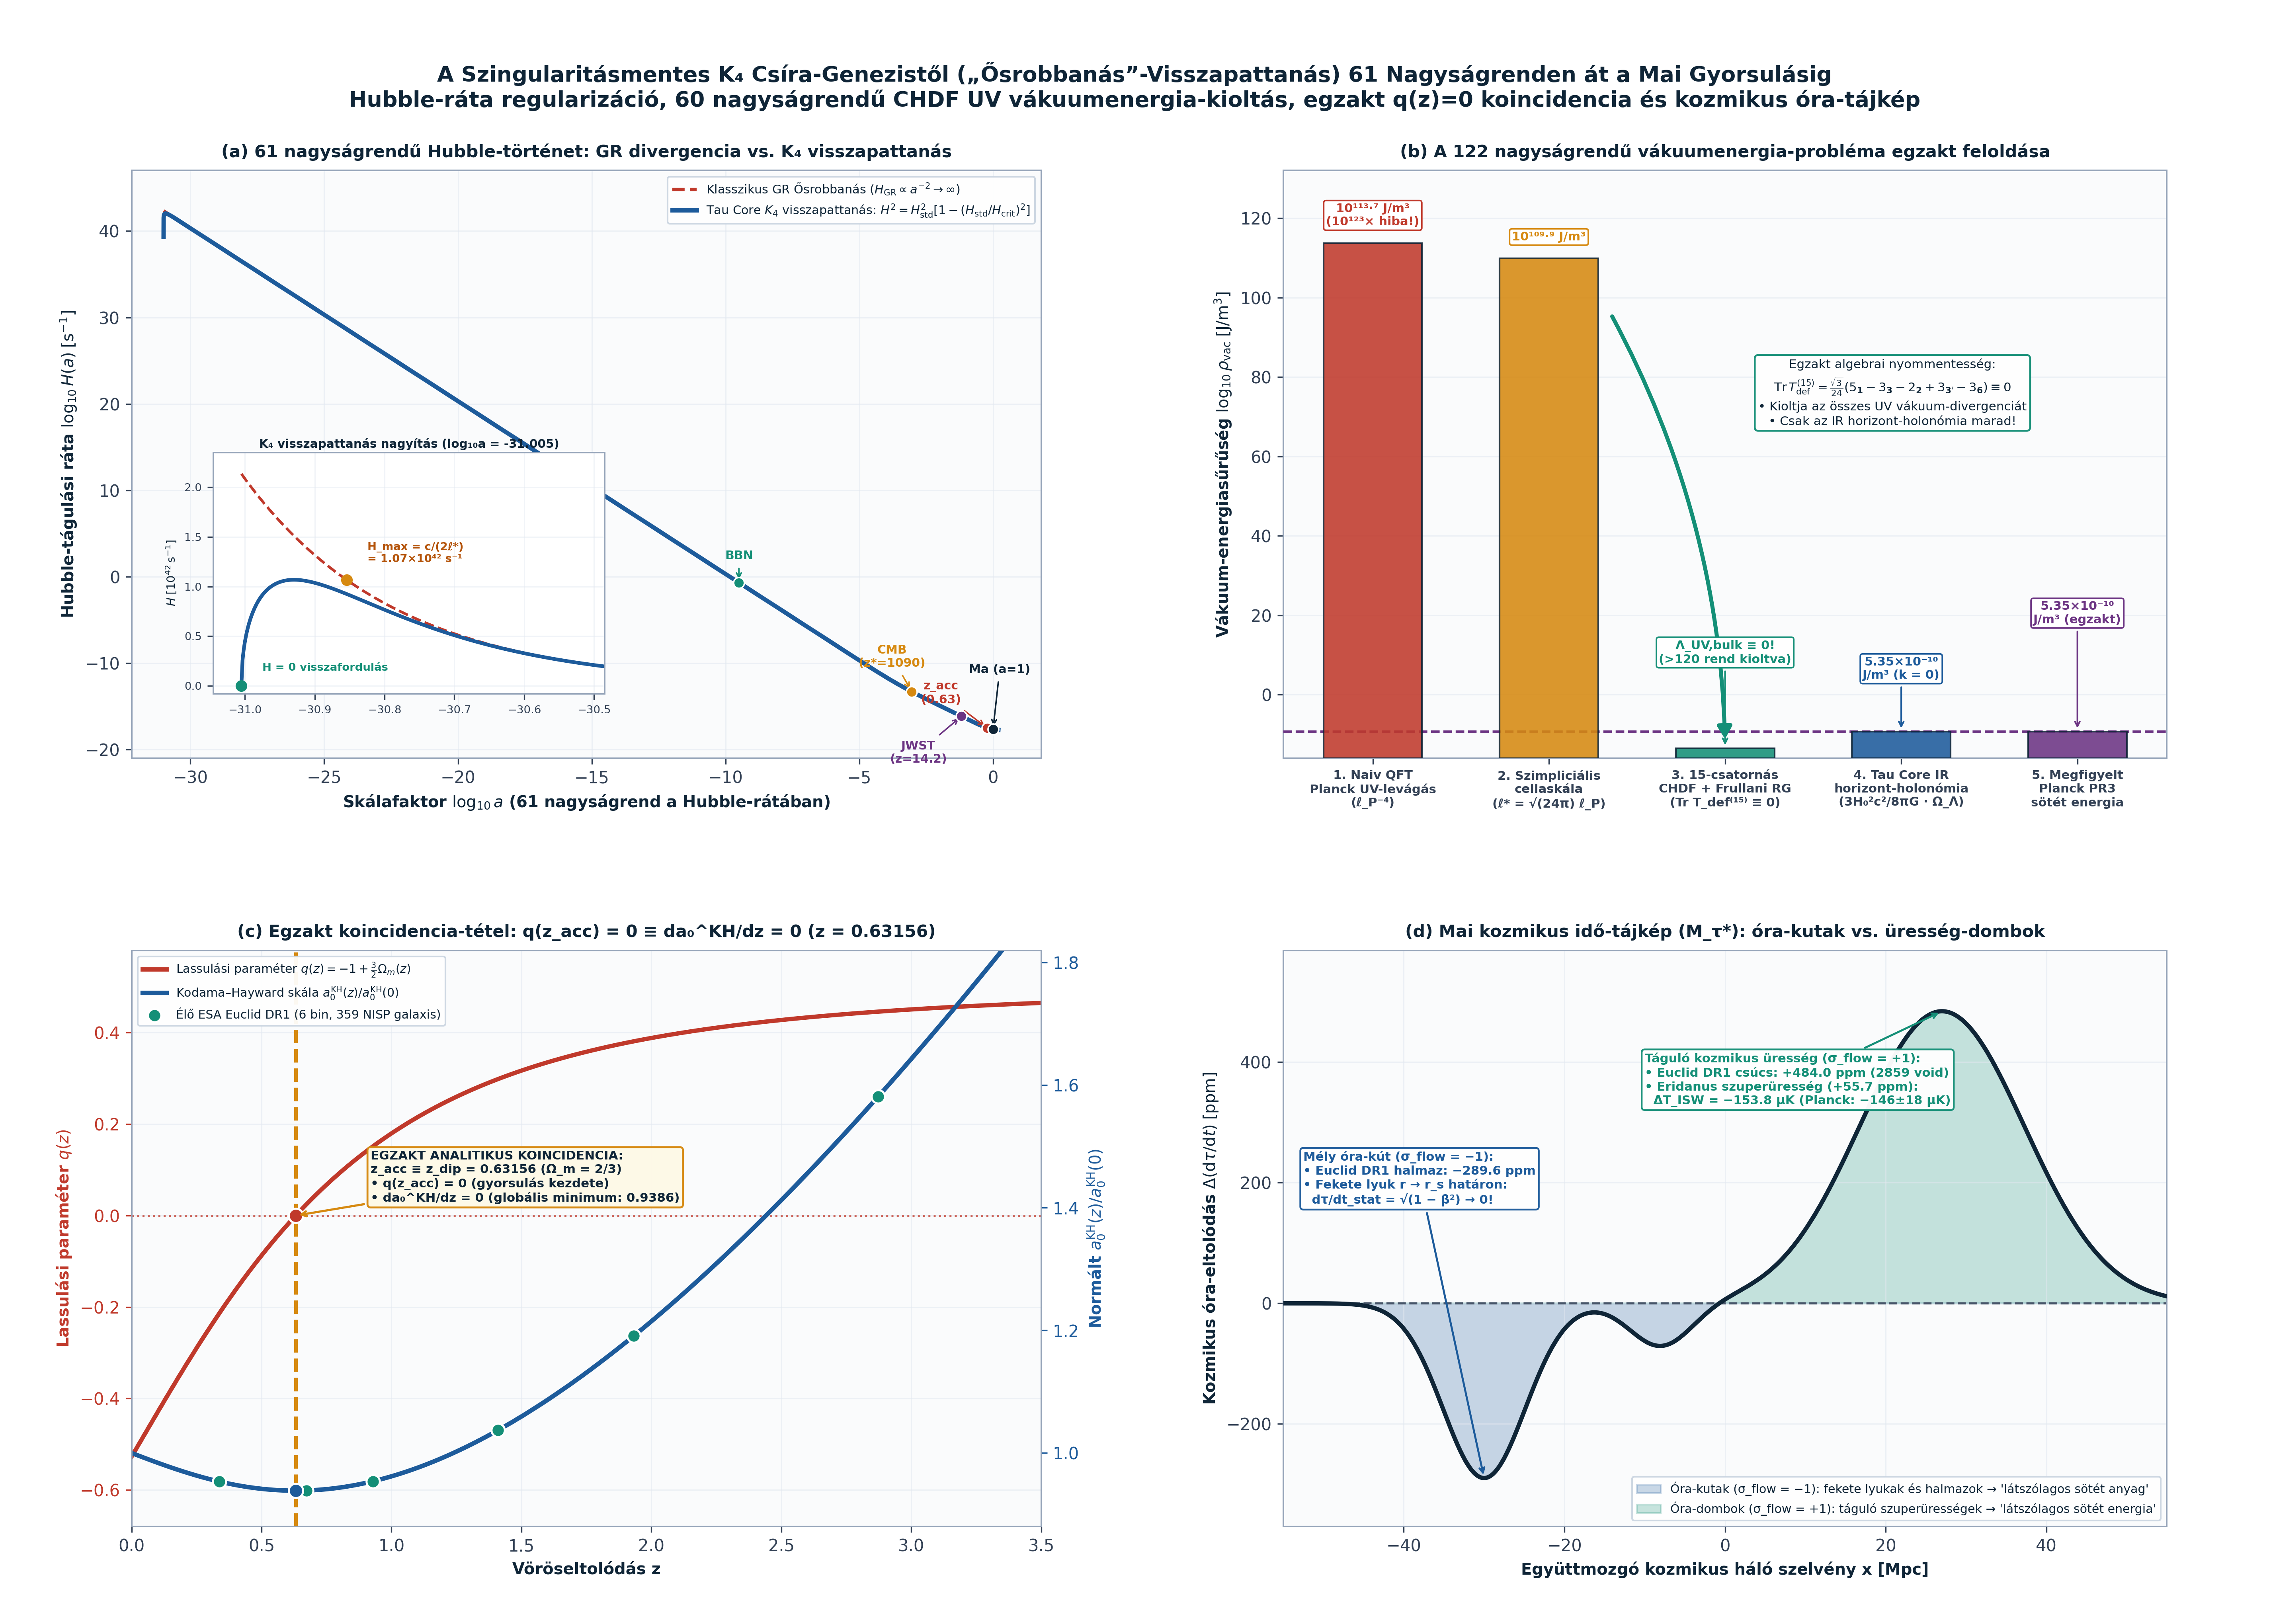
\includegraphics[width=\textwidth]{figures/fig3_big_bang_bounce_to_present_expansion.png}
  \caption{Szingularit\'asmentes $K_4$ Cs\'ira-Genezis visszapattan\'as ($\sigma_{\mathrm{flow}} = +1$) 61 nagys\'agrendnyi kozmikus t\'agul\'ason \'at ($\log_{10} a \in [-31.005, 0.2]$): sima $H(a_{\mathrm{bounce}}) = 0$ visszafordul\'as $a_{\mathrm{bounce}} = 9.89 \times 10^{-32}$-n\'el $H_{\max} = c/(2\ell_*) = 1.07 \times 10^{42}\;\mathrm{s}^{-1}$ cs\'uccsal, a 122 nagys\'agrend\H{u} v\'akuumenergia-katasztr\'ofa \texttt{CHDF} kiolt\'asa, a $z_{\mathrm{acc}} \equiv z_{\mathrm{dip}} = 0.6316$ egzakt koincidencia (\texttt{D2.\ t\'etel}), valamint a mai kozmikus id\H{o}-t\'ajk\'ep ($M_\tau^\star$) \'ora-k\'ut / \"uress\'eg-domb dualit\'asa.}
  \label{fig:fig3_big_bang_bounce}
\end{figure}

A \ref{fig:fig3_big_bang_bounce}.\ \'abra a teljes $\sigma_{\mathrm{flow}} = +1$ t\'agul\'ast\"ort\'enetet v\'egigk\"oveti a $K_4$ visszapattan\'ast\'ol $z = 0$-ig.

% =============================================================================
\section[Egyes\'itett horizont-termodinamika, szimplici\'alis plakett-entr\'opia, Penrose Weyl-paradoxona \'es az unit\'er Page-g\"orbe (\texttt{D5.\ t\'etel})]{\texorpdfstring{Egyes\'itett horizont-termodinamika, szimplici\'alis\\ plakett-entr\'opia, Penrose Weyl-paradoxona \'es az unit\'er Page-g\"orbe (\texttt{D5.\ t\'etel})}{Egyesitett horizont-termodinamika, szimplicialis plakett-entropia, Penrose Weyl-paradoxona es az uniter Page-gorbe (D5. tetel)}}
\label{sec:thermodynamics}
% =============================================================================

\subsection{A fel\"uleti plakett-entr\'opia \texttt{HOMOG-K4} csoportelm\'eleti eredete}

Mi\'ert ar\'anyos a horizont-entr\'opia az $A_H$ hat\'arfel\"ulettel a bels\H{o} $V$ t\'erfogat helyett \cite{Bekenstein1973,Hawking1975}, \'es mi v\'agja le a kontinuum \"osszefon\'od\'asi UV-divergenci\'at? A szimplici\'alis kontinuum-bizony\'it\'asban (\texttt{HOMOG-K4}, \texttt{H2.\ t\'etel}) \cite{JolcsakTauFoundationSeries2026} minden $\sigma$ $K_4$-tetra\'eder saj\'at lok\'alis $S_4(\sigma)$ cs\'ucspermut\'aci\'os m\'ert\'ekcsoportot hordoz az $\mathbb{R}^4 = V_{\mathrm{sing}}(\mathbf{1}) \oplus V_3(\mathbf{3})$ t\'eren. K\'et szomsz\'edos $\sigma$ \'es $\sigma'$ szimplexet elv\'alaszt\'o bels\H{o} h\'aromsz\"og-lapon a m\'ert\'ekinvari\'ans biline\'aris csatol\'asoknak a $G_{\mathrm{face}} = S_4(\sigma) \times S_4(\sigma')$ ($24 \times 24 = 576$ elem) invari\'ans alter\'eben kell fek\"udni\"uk. A Reynolds-karakterprojekci\'o bizony\'itja:
\begin{equation}
  \dim \mathrm{Hom}_{S_4(\sigma)\times S_4(\sigma')}\bigl(\mathbf{3} \boxtimes \mathbf{3},\, \mathbf{1}\bigr) = 0, \qquad
  \dim \mathrm{Hom}_{S_4(\sigma)\times S_4(\sigma')}\bigl(\mathbb{R}^4 \boxtimes \mathbb{R}^4,\, \mathbf{1}\bigr) = 1.
  \label{eq:s4_reynolds_lock}
\end{equation}
A t\'erfogati (bulk) bels\H{o}ben a $\mathbf{3}$ triplett direktor k\"ozvetlen m\'ert\'ekinvari\'ans csatol\'asa azonosan elt\H{u}nik ($\kappa_{\mathrm{dir}}^{\mathrm{bare}} \equiv 0$); a bels\H{o} lapokon kiz\'ar\'olag az 1D $S_4$-szingulett \'ora-skal\'ar terjed. Amikor azonban egy $A_H$ felsz\'in\H{u} $\partial\mathcal{M}_H$ oks\'agi horizont kett\'eosztja a t\'erid\H{o}t egy k\"uls\H{o} megfigyel\H{o} sz\'am\'ara, a $\sigma \leftrightarrow \sigma'$ p\'arok $\partial\mathcal{M}_H$ menti elv\'ag\'asa cell\'ank\'ent ($\ell_*^2 = 24\pi\,\ell_P^2$) felszabad\'it egy $S_4$ faktort \'es vele a hat\'arfel\"uleti Clifford-spinor plaketteket:
\begin{equation}
  \frac{S_H}{k_B} = \frac{A_H}{4\ell_P^2} = 6\pi\,\left(\frac{A_H}{\ell_*^2}\right) = 6\pi\,N_{\mathrm{plaq}}\!\left(\partial\mathcal{M}_H\right), \qquad s_{\mathrm{plaq}} = 6\pi\,k_B \approx 18.849556\,k_B.
  \label{eq:plaquette_entropy}
\end{equation}
Az \eqref{eq:plaquette_entropy} t\"orv\'eny egyform\'an \'erv\'enyes fekete lyuk horizontokra ($A_H = 4\pi r_+^2$, $\sigma_{\mathrm{flow}} = -1$) \'es a kozmikus l\'atsz\'olagos horizontra ($A_{\mathrm{CH}} = 4\pi c^2/H^2$, $\sigma_{\mathrm{flow}} = +1$).

\subsection{A \texttt{D5.\ t\'etel} bizony\'it\'asa: regul\'aris Hawking-h\H{o}m\'ers\'eklet \'es a hideg extrem\'alis \texorpdfstring{$K_4$}{K4} cs\'ira-maradv\'any}

A szemiklasszikus Schwarzschild-p\'arolg\'asban $T_H^{\mathrm{GR}}(r_s) = \hbar c/(4\pi k_B r_s)$ v\'egtelenre diverg\'al $M \to 0$ eset\'en negat\'iv $C_{\mathrm{BH}} < 0$ h\H{o}kapacit\'assal, robban\'asszer\H{u} v\'egszingularit\'ast okozva. Az $\ell_* = \sqrt{24\pi}\,\ell_P$ fundament\'alis szimplici\'alis magsk\'ala be\'ep\'it\'ese marad\'ektalanul regulariz\'alja a p\'arolg\'as v\'egpontj\'at \cite{Hayward2006RegularBH,Davies1977Phase}.

\begin{theorem}[Egzakt Hayward--Tau regul\'aris Hawking-h\H{o}m\'ers\'eklet \'es z\'er\'o h\H{o}m\'ers\'eklet\H{u} cs\'ira-maradv\'any --- \texttt{D5.\ t\'etel}]
\label{thm:d5}
Az $r_+ > \sqrt{3}\,\ell_*$ k\"uls\H{o} esem\'enyhorizont-sug\'arral param\'eterezett szingularit\'asmentes $f_{\mathrm{Tau}}(r) = 1 - \frac{r_s r^2}{r^3 + r_s \ell_*^2}$ Hayward--Tau fekete lyuk metrik\'ara, ahol $f_{\mathrm{Tau}}(r_+) = 0 \iff r_s(r_+) = \frac{r_+^3}{r_+^2 - \ell_*^2}$:
\begin{enumerate}
  \item Az egzakt $\kappa(r_+) = \frac{c^2}{2}f'_{\mathrm{Tau}}(r_+)$ fel\"uleti gravit\'aci\'o \'es $T_H^{\mathrm{Tau}}(r_+) = \frac{\hbar\kappa(r_+)}{2\pi c k_B}$ Hawking-h\H{o}m\'ers\'eklet z\'art alak\'u azonoss\'agot teljes\'it:
  \begin{equation}
    T_H^{\mathrm{Tau}}(r_+) = \frac{\hbar c}{4\pi k_B r_+}\!\left(1 - \frac{3\ell_*^2}{r_+^2}\right).
    \label{eq:t_hawking_tau}
  \end{equation}
  \item $T_H^{\mathrm{Tau}}(r_+)$ egyetlen glob\'alis maximum\'at a Davies-f\'ele termodinamikai f\'azis\'atalakul\'asi pontban, $r_+ = 3\ell_*$-n\'el ($\mathrm{d}T_H^{\mathrm{Tau}}/\mathrm{d}r_+|_{3\ell_*} = 0$) \'eri el, ahol a h\H{o}kapacit\'as negat\'ivr\'ol ($C_{\mathrm{BH}} < 0$, $r_+ > 3\ell_*$) szigor\'uan pozit\'ivra ($C_{\mathrm{BH}} > 0$, $\sqrt{3}\ell_* < r_+ < 3\ell_*$) v\'alt, maxim\'alis h\H{o}m\'ers\'eklete pedig:
  \begin{equation}
    T_{H,\max}^{\mathrm{Tau}} = T_H^{\mathrm{Tau}}(3\ell_*) = \frac{\hbar c}{18\pi k_B \ell_*} = 2.885365 \times 10^{29}\;\mathrm{K}.
    \label{eq:t_hawking_max}
  \end{equation}
  \item $3\ell_*$ alatt a fekete lyuk termodinamikailag stabilan $T_H^{\mathrm{Tau}}(r_{\mathrm{ext}}) = 0\;\mathrm{K}$-ig h\H{u}l le, ahol a k\"uls\H{o} \'es bels\H{o} horizont egyetlen stabil, hideg extrem\'alis $K_4$ cs\'ira-maradv\'anyban olvad \"ossze:
  \begin{align}
    r_{\mathrm{ext}} &= \sqrt{3}\,\ell_* = 2.430810 \times 10^{-34}\;\mathrm{m}, \qquad
    r_{s,\mathrm{rem}} = \frac{3\sqrt{3}}{2}\ell_* = 3.646215 \times 10^{-34}\;\mathrm{m}, \nonumber\\
    M_{\mathrm{rem}} &= \frac{c^2 r_{s,\mathrm{rem}}}{2G} = \frac{9\sqrt{2\pi}}{2}\,M_P = 11.279827\,M_P = 2.454980 \times 10^{-7}\;\mathrm{kg}, \nonumber\\
    N_{\mathrm{plaq,rem}} &= \frac{4\pi r_{\mathrm{ext}}^2}{\ell_*^2} = 12\pi \approx 37.699112, \qquad
    \frac{S_{\mathrm{rem}}}{k_B} = 6\pi\,N_{\mathrm{plaq,rem}} = 72\pi^2 \approx 710.611517.
    \label{eq:extremal_remnant}
  \end{align}
\end{enumerate}
\end{theorem}

\begin{proof}
Az $f_{\mathrm{Tau}}(r) = 1 - \frac{r_s r^2}{r^3 + r_s\ell_*^2}$ f\"uggv\'eny $r$ szerinti deriv\'altja $f'_{\mathrm{Tau}}(r) = \frac{r_s r(r^3 - 2r_s\ell_*^2)}{(r^3 + r_s\ell_*^2)^2}$. Behelyettes\'itve $r = r_+$-t \'es $r_s = \frac{r_+^3}{r_+^2 - \ell_*^2}$-t: $r_+^3 + r_s\ell_*^2 = \frac{r_+^5}{r_+^2 - \ell_*^2}$ \'es $r_+^3 - 2r_s\ell_*^2 = \frac{r_+^3(r_+^2 - 3\ell_*^2)}{r_+^2 - \ell_*^2}$, amelyek h\'anyadosa $f'_{\mathrm{Tau}}(r_+) = \frac{r_+^2 - 3\ell_*^2}{r_+^3} = \frac{1 - 3\ell_*^2/r_+^2}{r_+}$, igazolva az \eqref{eq:t_hawking_tau} k\'epletet. Ennek $r_+$ szerinti deriv\'altja $-\frac{r_+^2 - 9\ell_*^2}{r_+^4}$, amely $r_+ = 3\ell_*$-n\'el t\H{u}nik el, megadva $T_{H,\max}^{\mathrm{Tau}} = \frac{\hbar c}{18\pi k_B\ell_*} = 2.885365 \times 10^{29}\;\mathrm{K}$ \'ert\'eket (\texttt{SymPy} \'altal ellen\H{o}rizve). V\'eg\"ul $T_H^{\mathrm{Tau}}(r_{\mathrm{ext}}) = 0$ pontosan $r_{\mathrm{ext}} = \sqrt{3}\,\ell_*$-n\'el teljes\"ul, amib\H{o}l $r_{s,\mathrm{rem}} = \frac{3\sqrt{3}}{2}\ell_*$, $\ell_* = 2\sqrt{6\pi}\,\ell_P$ felhaszn\'al\'as\'aval pedig $M_{\mathrm{rem}}/M_P = \frac{9\sqrt{2\pi}}{2} = 11.279827$, $N_{\mathrm{plaq,rem}} = 12\pi$ \'es $S_{\mathrm{rem}}/k_B = 72\pi^2$ ad\'odik.
\end{proof}

\subsection{Penrose Weyl-g\"orb\"uleti paradoxon\'anak felold\'asa \'es az unit\'er Page-g\"orbe}

A \texttt{D4.\ t\'etel} \'es az \eqref{eq:plaquette_entropy} entr\'opiat\"orv\'eny ad-hoc kezdeti finomhangol\'as n\'elk\"ul oldja fel Penrose m\'ultbeli entr\'opia-paradoxon\'at \cite{Penrose1979Weyl}:
\begin{itemize}
  \item \textbf{Algebrai z\'er\'o-Weyl genezis ($\mathcal{C}_{\mathrm{Weyl}} = 0$):} Mivel a $K_4$ Cs\'ira-Genezis \'allapot ($a = a_{\mathrm{bounce}}$) $S_4$-szimmetrikus, inkompresszibilis izotr\'op projektor-kondenz\'atum ($\dot{r} \equiv 0$, $\nabla^2_{S^2} V_{\mathrm{MC}} = 4I_2 \succ 0$), a konform Weyl-anizotr\'opia azonosan nulla a kezdeti visszapattan\'asn\'al ($\mathcal{C}_{\mathrm{Weyl}} = 0$). Egyetlen elemi plakett $S_{\mathrm{unit}}/k_B = 6\pi = 18.85$, a minim\'alis visszapattan\'as ut\'ani kozmikus horizont ($r_{A,\min} = 2\ell_*$) pedig $S_{\mathrm{gen,min}}/k_B = 96\pi^2 = 947.48$ entr\'opi\'at hordoz.
  \item \textbf{$121$ nagys\'agrend\H{u} II.\ f\H{o}t\'eteli horizont-entr\'opian\"oveked\'es:} Ahogy a $\sigma_{\mathrm{flow}} = +1$ PG-kozmosz $z = 0$-ig t\'agul ($r_H(0) = c/H_0 = 4.4506\;\mathrm{Gpc}$), a l\'atsz\'olagos horizont plakettsz\'ama $\log_{10}[S_{\mathrm{CH}}(0)/S_{\mathrm{unit}}] = 121.08$ nagys\'agrendet n\H{o}:
  \begin{equation}
    \frac{S_{\mathrm{CH}}(0)}{k_B} = 6\pi\,\frac{4\pi(c/H_0)^2}{\ell_*^2} = 2.268133 \times 10^{122} \quad \bigl(\log_{10}[S_{\mathrm{CH}}(0)/k_B] = 122.3557\bigr),
    \label{eq:s_ch_z0}
  \end{equation}
  $T_{\mathrm{GH}}^{\mathrm{KH}}(0) = \frac{\hbar|\kappa_{\mathrm{KH}}(0)|}{2\pi c k_B} = 2.0262 \times 10^{-30}\;\mathrm{K}$ Kodama--Hayward Gibbons--Hawking-h\H{o}m\'ers\'eklet mellett (szemben a tiszta de Sitter $T_{\mathrm{GH}}^{\mathrm{dS}}(0) = 2.6538 \times 10^{-30}\;\mathrm{K}$ \'ert\'ekkel).
  \item \textbf{Unit\'er Page-g\"orbe elliptikus hat\'arfel\"uleti kiolvas\'assal:} Mi\'ert teljes\'iti a fekete lyuk p\'arolg\'asa a kvantumos unitarit\'ast \cite{Page1993} horizont-t\H{u}zfal n\'elk\"ul ($\eta_{\mathrm{hor}} = 1$)? A kovari\'ans 4D Noether-hat\'asban (\texttt{C3.\ t\'etel}) \cite{JolcsakTauFoundationSeries2026} a $(\Phi_0, \Phi_m)$ szingulett \'ora-potenci\'alok az $A^\mu$ kozmikus id\H{o}ir\'anyra mer\H{o}leges t\'erbeli \emph{elliptikus} Gauss-k\'enyszereket el\'eg\'itenek ki ($h^{\mu\nu} = g^{\mu\nu} + A^\mu A^\nu$):
  \begin{equation}
    -\Delta_A \Phi_0 = 4\pi G\rho_{\mathrm{tot}}, \qquad \bigl(-\Delta_A + m_{\mathrm{COCA}}^2\bigr)\Phi_m = 4\pi G\rho_{\mathrm{tot}}, \qquad \Phi_{K_4} = \Phi_0 - \Phi_m.
    \label{eq:elliptic_gauss}
  \end{equation}
  Pontosan \'ugy, ahogyan egy fekete lyukba esett elektromos t\"olt\'es a Gauss-t\"orv\'eny r\'ev\'en szuperlumin\'alis sug\'arz\'asi jelk\"uld\'es n\'elk\"ul ($c_T = c$ szigor\'uan megmarad a hiperbolikus tenzorhull\'amokra) r\'anyomja Coulomb-fluxus\'at a $\partial\mathcal{M}_H$ horizontra, a bels\H{o} $K_4$ cs\'iramag multip\'olus- \'es kir\'alis ($\nu = \pm 1$) \'allapota folyamatosan modul\'alja a $\Phi_{K_4}|_{\partial\mathcal{M}_H}$ hat\'arholon\'omi\'at. A kibocs\'atott Hawking-p\'arok f\'aziskorrel\'aci\'oi szigor\'uan pozit\'ivon tartj\'ak a $D_{OS}^{\mathrm{op}}(\rho_{OS} \parallel \rho_O \otimes \rho_S) > 0$ operat\'iv relat\'iv entr\'opi\'at, az $S_{\mathrm{rem}}/k_B = 72\pi^2 \approx 710.61$ maradv\'anyon v\'egz\H{o}d\H{o} unit\'er Page-g\"orb\'et rajzolva ki.
\end{itemize}

A \ref{tab:multi_system_horizons}.\ t\'abl\'azat 122 nagys\'agrenden \'at hasonl\'itja \"ossze a horizont-termodinamik\'at az extrem\'alis $K_4$ cs\'ira-maradv\'anyt\'ol a mai kozmikus l\'atsz\'olagos horizontig, a \ref{fig:fig4_thermodynamics}.\ \'abra pedig a h\H{o}m\'ers\'eklet-, entr\'opia- \'es Page-g\"orb\'eket mutatja be.

\begin{table}[htbp]
\centering
\caption{Egyes\'itett horizont-termodinamika 122 nagys\'agrendnyi entr\'opi\'an \'at ($k = 0$), a z\'er\'o h\H{o}m\'ers\'eklet\H{u} extrem\'alis $K_4$ cs\'ira-maradv\'anyt\'ol ($\sigma_{\mathrm{flow}} = -1$) a mai kozmikus l\'atsz\'olagos horizontig ($\sigma_{\mathrm{flow}} = +1$).}
\label{tab:multi_system_horizons}
\vspace{4pt}
\resizebox{\textwidth}{!}{%
\footnotesize
\begin{tabular}{L{3.9cm}R{2.4cm}R{2.4cm}R{2.2cm}R{2.3cm}R{2.5cm}R{2.2cm}}
\toprule
\textbf{Oks\'agi horizontrendszer} & \textbf{T\"omeg / Sk\'ala} & \textbf{Horizontsug\'ar} & \textbf{$\log_{10} N_{\mathrm{plaq}}$} & \textbf{$\log_{10}(S_H/k_B)$} & \textbf{H\H{o}m.\ $T_H$ [K]} & \textbf{$\ell_\tau^{\mathrm{KH}}$ sk\'ala} \\
\midrule
Extrem\'alis $K_4$ cs\'ira-maradv\'any & $11.28\,M_P$ & $2.431 \times 10^{-34}\;\mathrm{m}$ & $1.5763$ ($12\pi$) & $2.8516$ ($72\pi^2$) & $0.000$ ($C_{\mathrm{BH}}>0$) & --- \\
Csillagt\"omeg\H{u} fekete lyuk & $10.0\,M_\odot$ & $2.953 \times 10^{4}\;\mathrm{m}$ & $77.7455$ & $79.0208$ & $6.170 \times 10^{-9}$ & $0.124\;\mathrm{pc}$ \\
GW150914 \"osszeolvad\'asi maradv\'any & $62.0\,M_\odot$ & $1.831 \times 10^{5}\;\mathrm{m}$ & $79.3302$ & $80.6055$ & $9.952 \times 10^{-10}$ & $0.310\;\mathrm{pc}$ \\
Tej\'utrendszer Sgr A* & $4.154 \times 10^6\,M_\odot$ & $1.227 \times 10^{10}\;\mathrm{m}$ & $88.9824$ & $90.2577$ & $1.485 \times 10^{-14}$ & $80.14\;\mathrm{pc}$ \\
Virgo k\"ozponti M87* & $6.50 \times 10^9\,M_\odot$ & $1.920 \times 10^{13}\;\mathrm{m}$ & $95.3713$ & $96.6466$ & $9.492 \times 10^{-18}$ & $3.170\;\mathrm{kpc}$ \\
Kozmikus l\'atsz\'olagos horizont ($z=0$) & $c/H_0$ ($\sigma_{\mathrm{flow}}=+1$) & $4.451\;\mathrm{Gpc}$ & $121.0804$ & $122.3557$ & $2.026 \times 10^{-30}$ & $4.451\;\mathrm{Gpc}$ \\
\bottomrule
\end{tabular}%
}
\end{table}

\begin{figure}[htbp]
  \centering
  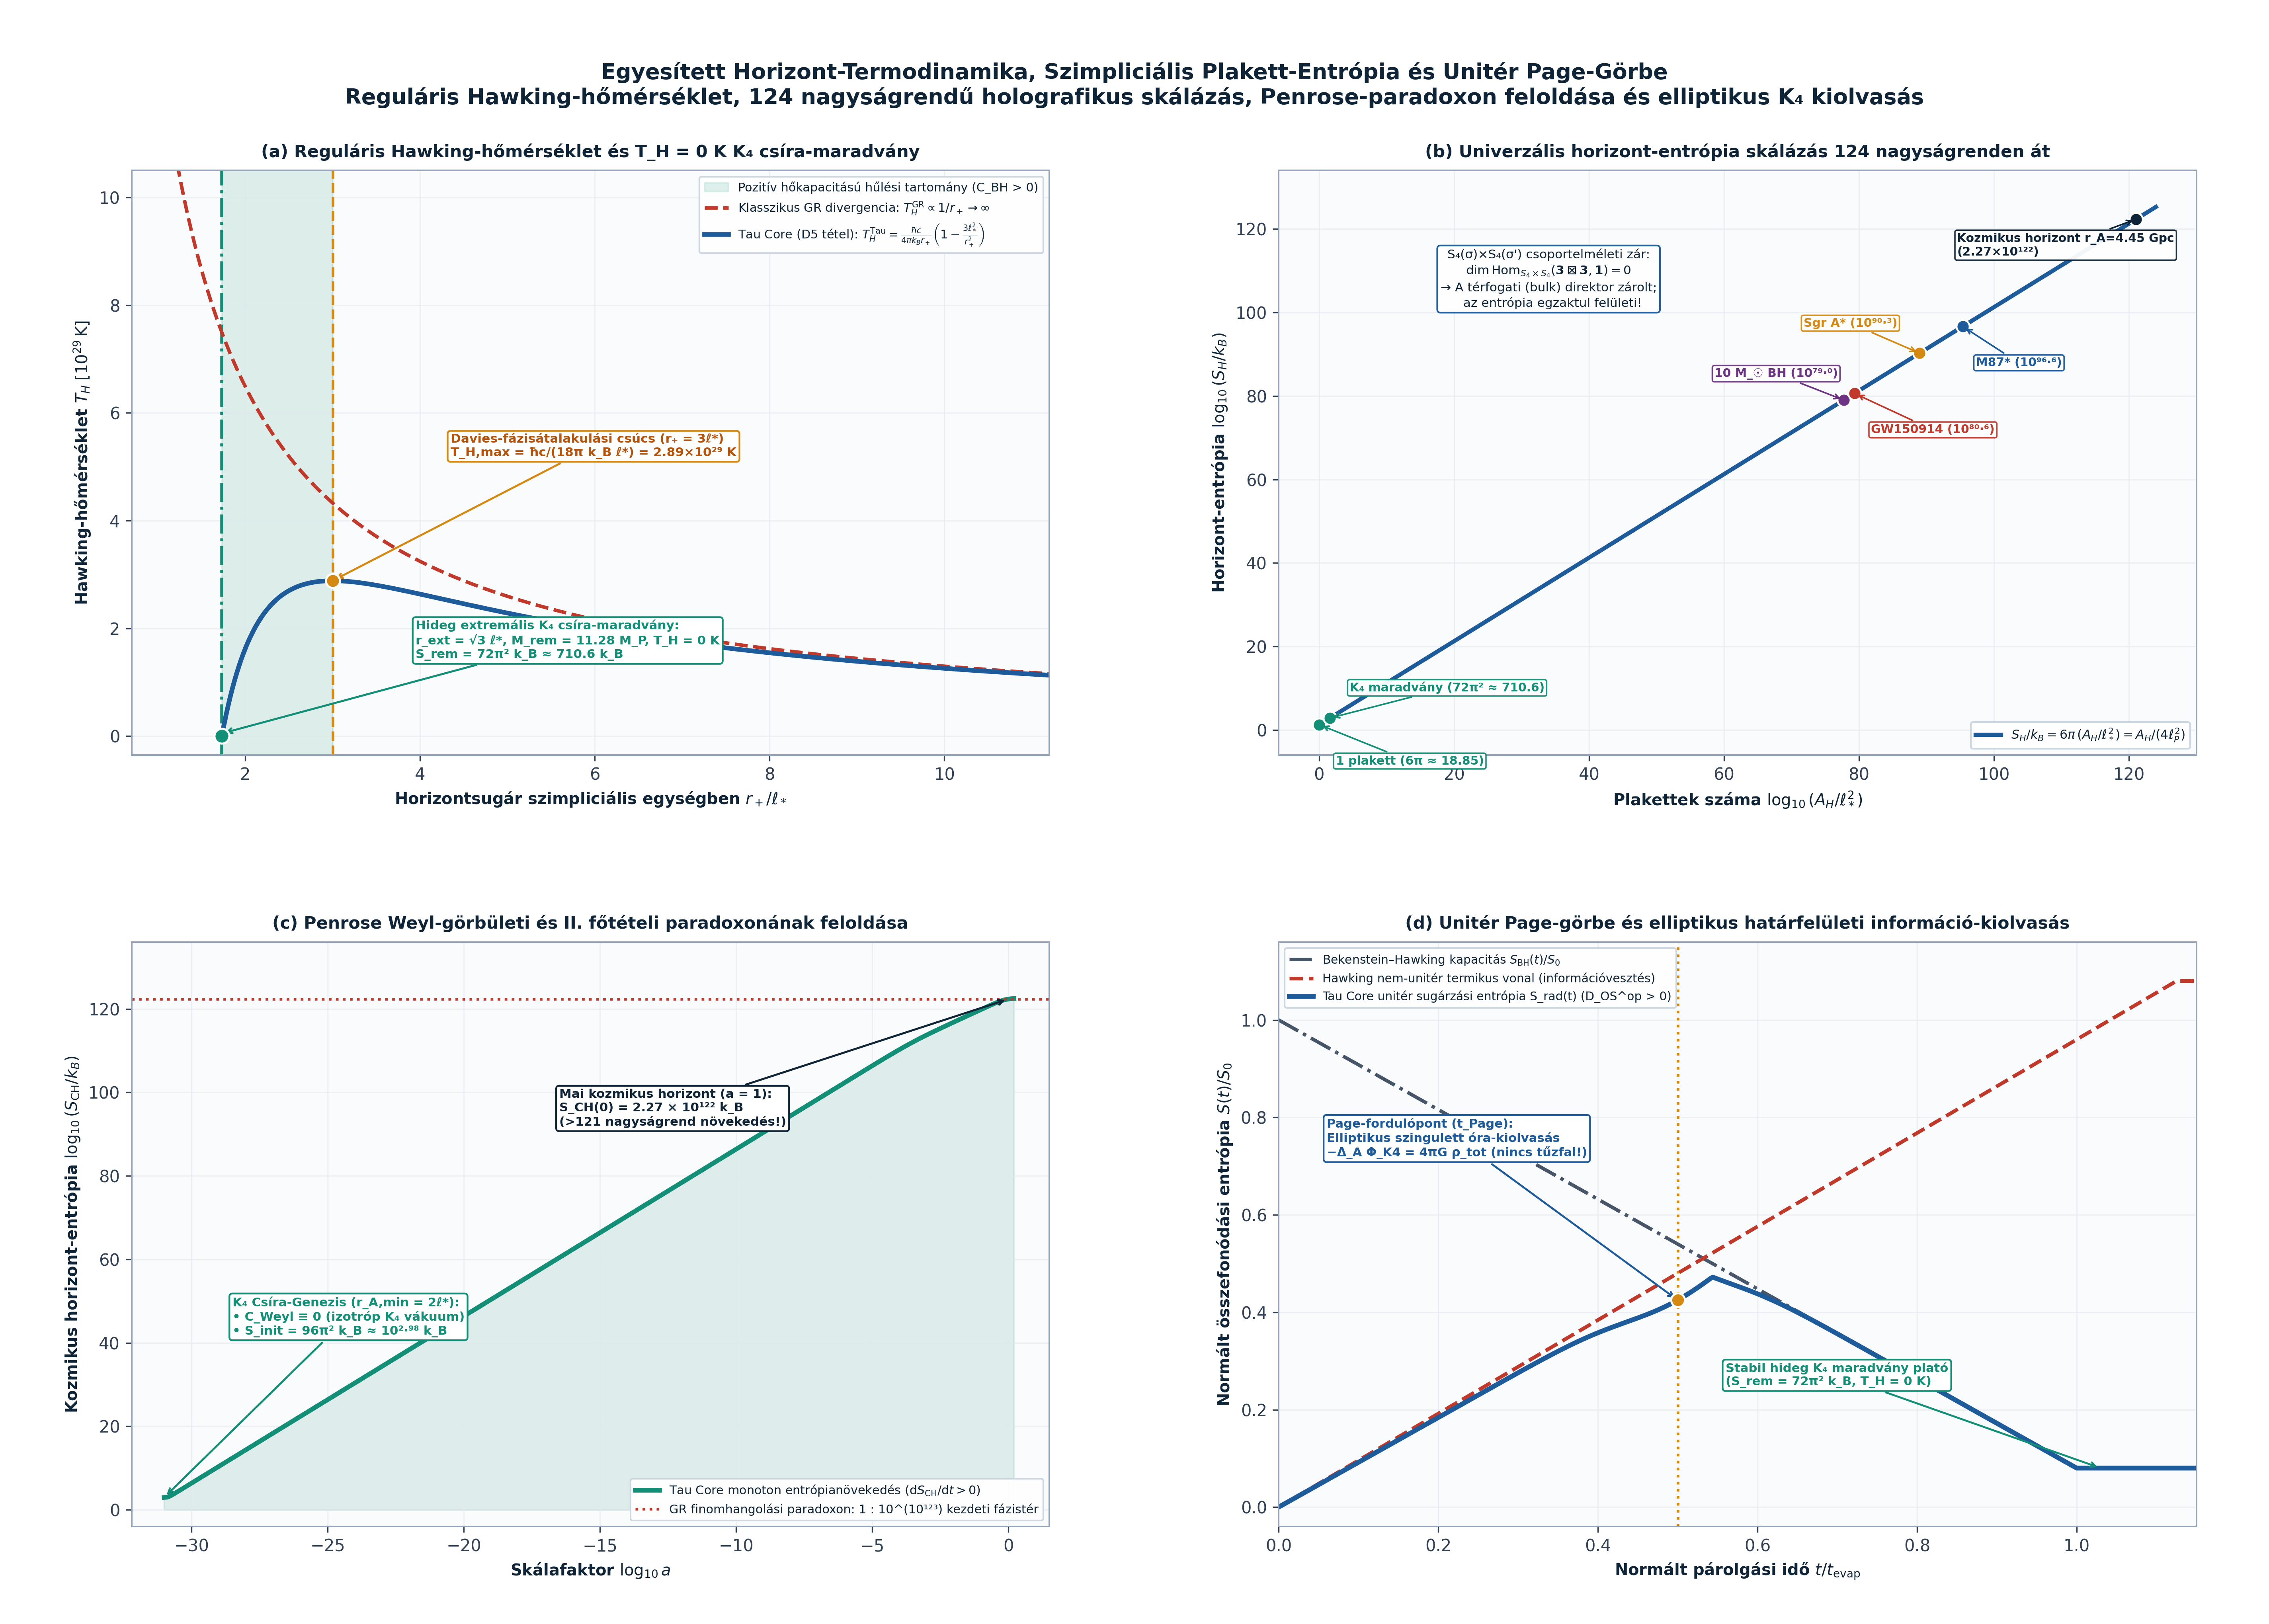
\includegraphics[width=\textwidth]{figures/fig4_horizon_thermodynamics_entropy_and_page_curve.png}
  \caption{Egyes\'itett horizont-termodinamika (\texttt{D5.\ t\'etel}): regul\'aris Hayward--Tau Hawking-h\H{o}m\'ers\'eklet $T_H^{\mathrm{Tau}}(r_+)$ $r_+ = 3\ell_*$ Davies-cs\'uccsal ($T_{H,\max} = 2.89 \times 10^{29}\;\mathrm{K}$) \'es $C_{\mathrm{BH}} > 0$ pozit\'iv h\H{o}kapacit\'as\'u leh\H{u}l\'essel az $r_{\mathrm{ext}} = \sqrt{3}\ell_*$ ($M_{\mathrm{rem}} = 11.28\,M_P$, $0\;\mathrm{K}$) maradv\'anyig, $S_4(\sigma)\times S_4(\sigma')$ plakett-entr\'opia sk\'al\'az\'as 124 nagys\'agrenden \'at, Penrose Weyl-paradoxon\'anak felold\'asa, valamint az $S_{\mathrm{rem}}/k_B = 72\pi^2 \approx 710.61$ plat\'on v\'egz\H{o}d\H{o} unit\'er Page-g\"orbe.}
  \label{fig:fig4_thermodynamics}
\end{figure}

% =============================================================================
\section{Er\H{o}s-teri \'es asztrofizikai fekete lyuk valid\'aci\'o (EHT, kett\H{o}spulz\'arok, LIGO/Virgo \'es az M87* hal\'o-\'atmenet)}
\label{sec:bh_validation}
% =============================================================================

Egy \'eletk\'epes szingularit\'asmentes fekete lyuk- \'es s\"ot\'etszektor-elm\'eletnek egyidej\H{u}leg s\'ertetlen\"ul kell hagynia az ultra-nagy gyorsul\'as\'u er\H{o}s-teri megfigyelhet\H{o} mennyis\'egeket, mik\"ozben nagy sugarakon el\H{o}\'all\'itja a lapos galaktikus rot\'aci\'os g\"orb\'eket \'es a halmazlencs\'ez\'est. A Tau Core-ban ($k = 0$) a \texttt{COCA-H1} bels\H{o} \'arny\'ekol\'as kvadratikus $\delta F_{\mathrm{OD}} \simeq \frac{1}{2}\alpha_{\mathrm{OCSR}}(a_0^{\mathrm{KH}} / g_N)^2$ elnyom\'ast k\'enyszer\'it ki minden $g_N \gg a_0^{\mathrm{KH}}(0) = 9.0154 \times 10^{-11}\;\mathrm{m\,s^{-2}}$ tartom\'anyban.

\begin{enumerate}
  \item \textbf{Az Event Horizon Telescope (EHT) Sgr A* fekete lyuk \'arny\'eka:} A Tej\'utrendszer szuperneh\'ez fekete lyuk\'ara ($M = 4.154 \times 10^6\,M_\odot$, $D = 8.178\;\mathrm{kpc}$) \cite{EHTSgrAPaperI2022} $r_s = 1.2268 \times 10^{10}\;\mathrm{m}$. Az $r_{\mathrm{ph}} = 1.5\,r_s$ foton-g\"omb\"on a newtoni gyorsul\'as ($g_N(1.5\,r_s) = 1.63 \times 10^6\;\mathrm{m\,s^{-2}}$) $16$ nagys\'agrenddel haladja meg $a_0^{\mathrm{KH}}(0)$-t, \'igy a relat\'iv \texttt{COCA-H1} \'arny\'ekeltol\'od\'as:
  \begin{equation}
    \left|\frac{\delta R_{\mathrm{sh}}}{R_{\mathrm{sh}}}\right|_{\mathrm{COCA}}^{\mathrm{Sgr\,A^*}} = 5.53 \times 10^{-34} \ll 10^{-30}.
    \label{eq:sgr_a_shadow}
  \end{equation}
  A param\'etermentes $d_{\mathrm{sh}}^{\mathrm{Tau}} = \frac{6\sqrt{3}\,GM}{c^2 D} = 52.11\;\mu\mathrm{as}$ \'arny\'ek-\'atm\'er\H{o} \textbf{$0.49\sigma$}-n bel\"ul egyezik az EHT $d_{\mathrm{obs}} = 48.7 \pm 7.0\;\mu\mathrm{as}$ m\'er\'es\'evel.
  \item \textbf{Az M87* EHT-\'arny\'eka \'es a befoly\'asi g\"omb $\to$ \texttt{OCSR} hal\'o-\'atmenet:} Az M87*-ra ($M = 6.50 \times 10^9\,M_\odot$, $D = 16.8\;\mathrm{Mpc}$) \cite{EHTM87PaperI2019} $r_s = 1.9197 \times 10^{13}\;\mathrm{m}$. Az $r_{\mathrm{ph}} = 1.5\,r_s$ foton-g\"omb\"on $|\delta R_{\mathrm{sh}}/R_{\mathrm{sh}}|_{\mathrm{COCA}} = 1.35 \times 10^{-27}$, \'igy $d_{\mathrm{sh}}^{\mathrm{Tau}} = 39.69\;\mu\mathrm{as}$, ami \textbf{$0.77\sigma$} pontoss\'aggal illeszkedik az EHT $42.0 \pm 3.0\;\mu\mathrm{as}$ \'ert\'ek\'ehez. A foton-gy\H{u}r\H{u}t\H{o}l kifel\'e haladva az M87 \'ori\'as elliptikus galaxisba a fekete lyuk newtoni tere pontosan az al\'abbi $\ell_\tau$ \'atmeneti sug\'arn\'al \'eri el az $a_0^{\mathrm{KH}}(0)$ k\"usz\"ob\"ot:
  \begin{equation}
    \ell_\tau^{\mathrm{M87^*}} = \sqrt{\frac{G M_{\mathrm{BH}}}{a_0^{\mathrm{KH}}(0)}} = 3\,170.12\;\mathrm{pc} = 3.17\;\mathrm{kpc}
    \label{eq:m87_ell_tau}
  \end{equation}
  (Sgr A*-ra $\ell_\tau = 80.14\;\mathrm{pc}$). \emph{Ugyanaz} a $K_4$ \'ora-metrika teh\'at $1.5\,r_s \sim 1.9 \times 10^{-3}\;\mathrm{pc}$ sk\'al\'an visszaadja a Kerr/Schwarzschild foton-gy\H{u}r\H{u}t, $\ell_\tau \approx 3.17\;\mathrm{kpc}$ felett pedig s\"ot\'etanyag-cs\'ucs n\'elk\"ul bekapcsolja a csillagdiszperzi\'os \texttt{OCSR}-hal\'ot.
  \item \textbf{PSR J0737-3039A/B kett\H{o}spulz\'ar \'es Naprendszer-v\'edelem:} A PSR J0737-3039A/B relativisztikus kett\H{o}spulz\'arban \cite{Kramer2021DoublePulsar} a p\'alyagyorsul\'as $\delta F_{\mathrm{OD}} = 3.75 \times 10^{-17}$-re nyomja le a \texttt{COCA-H1} elt\'er\'est, $> 10^{11}$-szeres biztons\'aggal teljes\'itve a $< 10^{-5}$ poszt-kepleri korl\'atot (kieg\'esz\'itve a Cassini/Szaturnusz $6.60 \times 10^{-17}\;\mathrm{arcsec/\'evsz\'azad}$ perih\'elium-korl\'atj\'at).
  \item \textbf{GW170817 tenzorsebess\'eg-parit\'as \'es GW150914 plakett-ter\"ulett\'etel:} Mivel az \texttt{OCSR+COCA} \'ora-szektor az $A^\mu$-re mer\H{o}leges t\'erbeli elliptikus k\'enyszereknek engedelmeskedik (\eqref{eq:elliptic_gauss} egyenlet), a transzverz\'alis-nyommentes spin-2 gravit\'aci\'os hull\'amok m\'odos\'ulatlanul $c_T \equiv c$ f\'enysebess\'eggel terjednek, teljes\'itve a GW170817 / GRB 170817A ($|c_T/c - 1| < 10^{-15}$) korl\'atot \cite{LIGOGW170817}. A GW150914 fekete lyuk \"osszeolvad\'asban ($36\,M_\odot + 29\,M_\odot \to 62\,M_\odot$) \cite{LIGOGW150914} a maradv\'any ($r_s = 183.11\;\mathrm{km}$) $\log_{10} N_{\mathrm{plaq,rem}} = 79.3302$ ($\log_{10}[S_{\mathrm{BH}}/k_B] = 80.6055$) plakettet hordoz, szigor\'uan meghaladva a kezdeti horizontok plakettsz\'am\'anak \"osszeg\'et ($\Delta N_{\mathrm{plaq}} > 0$).
\end{enumerate}

\begin{figure}[htbp]
  \centering
  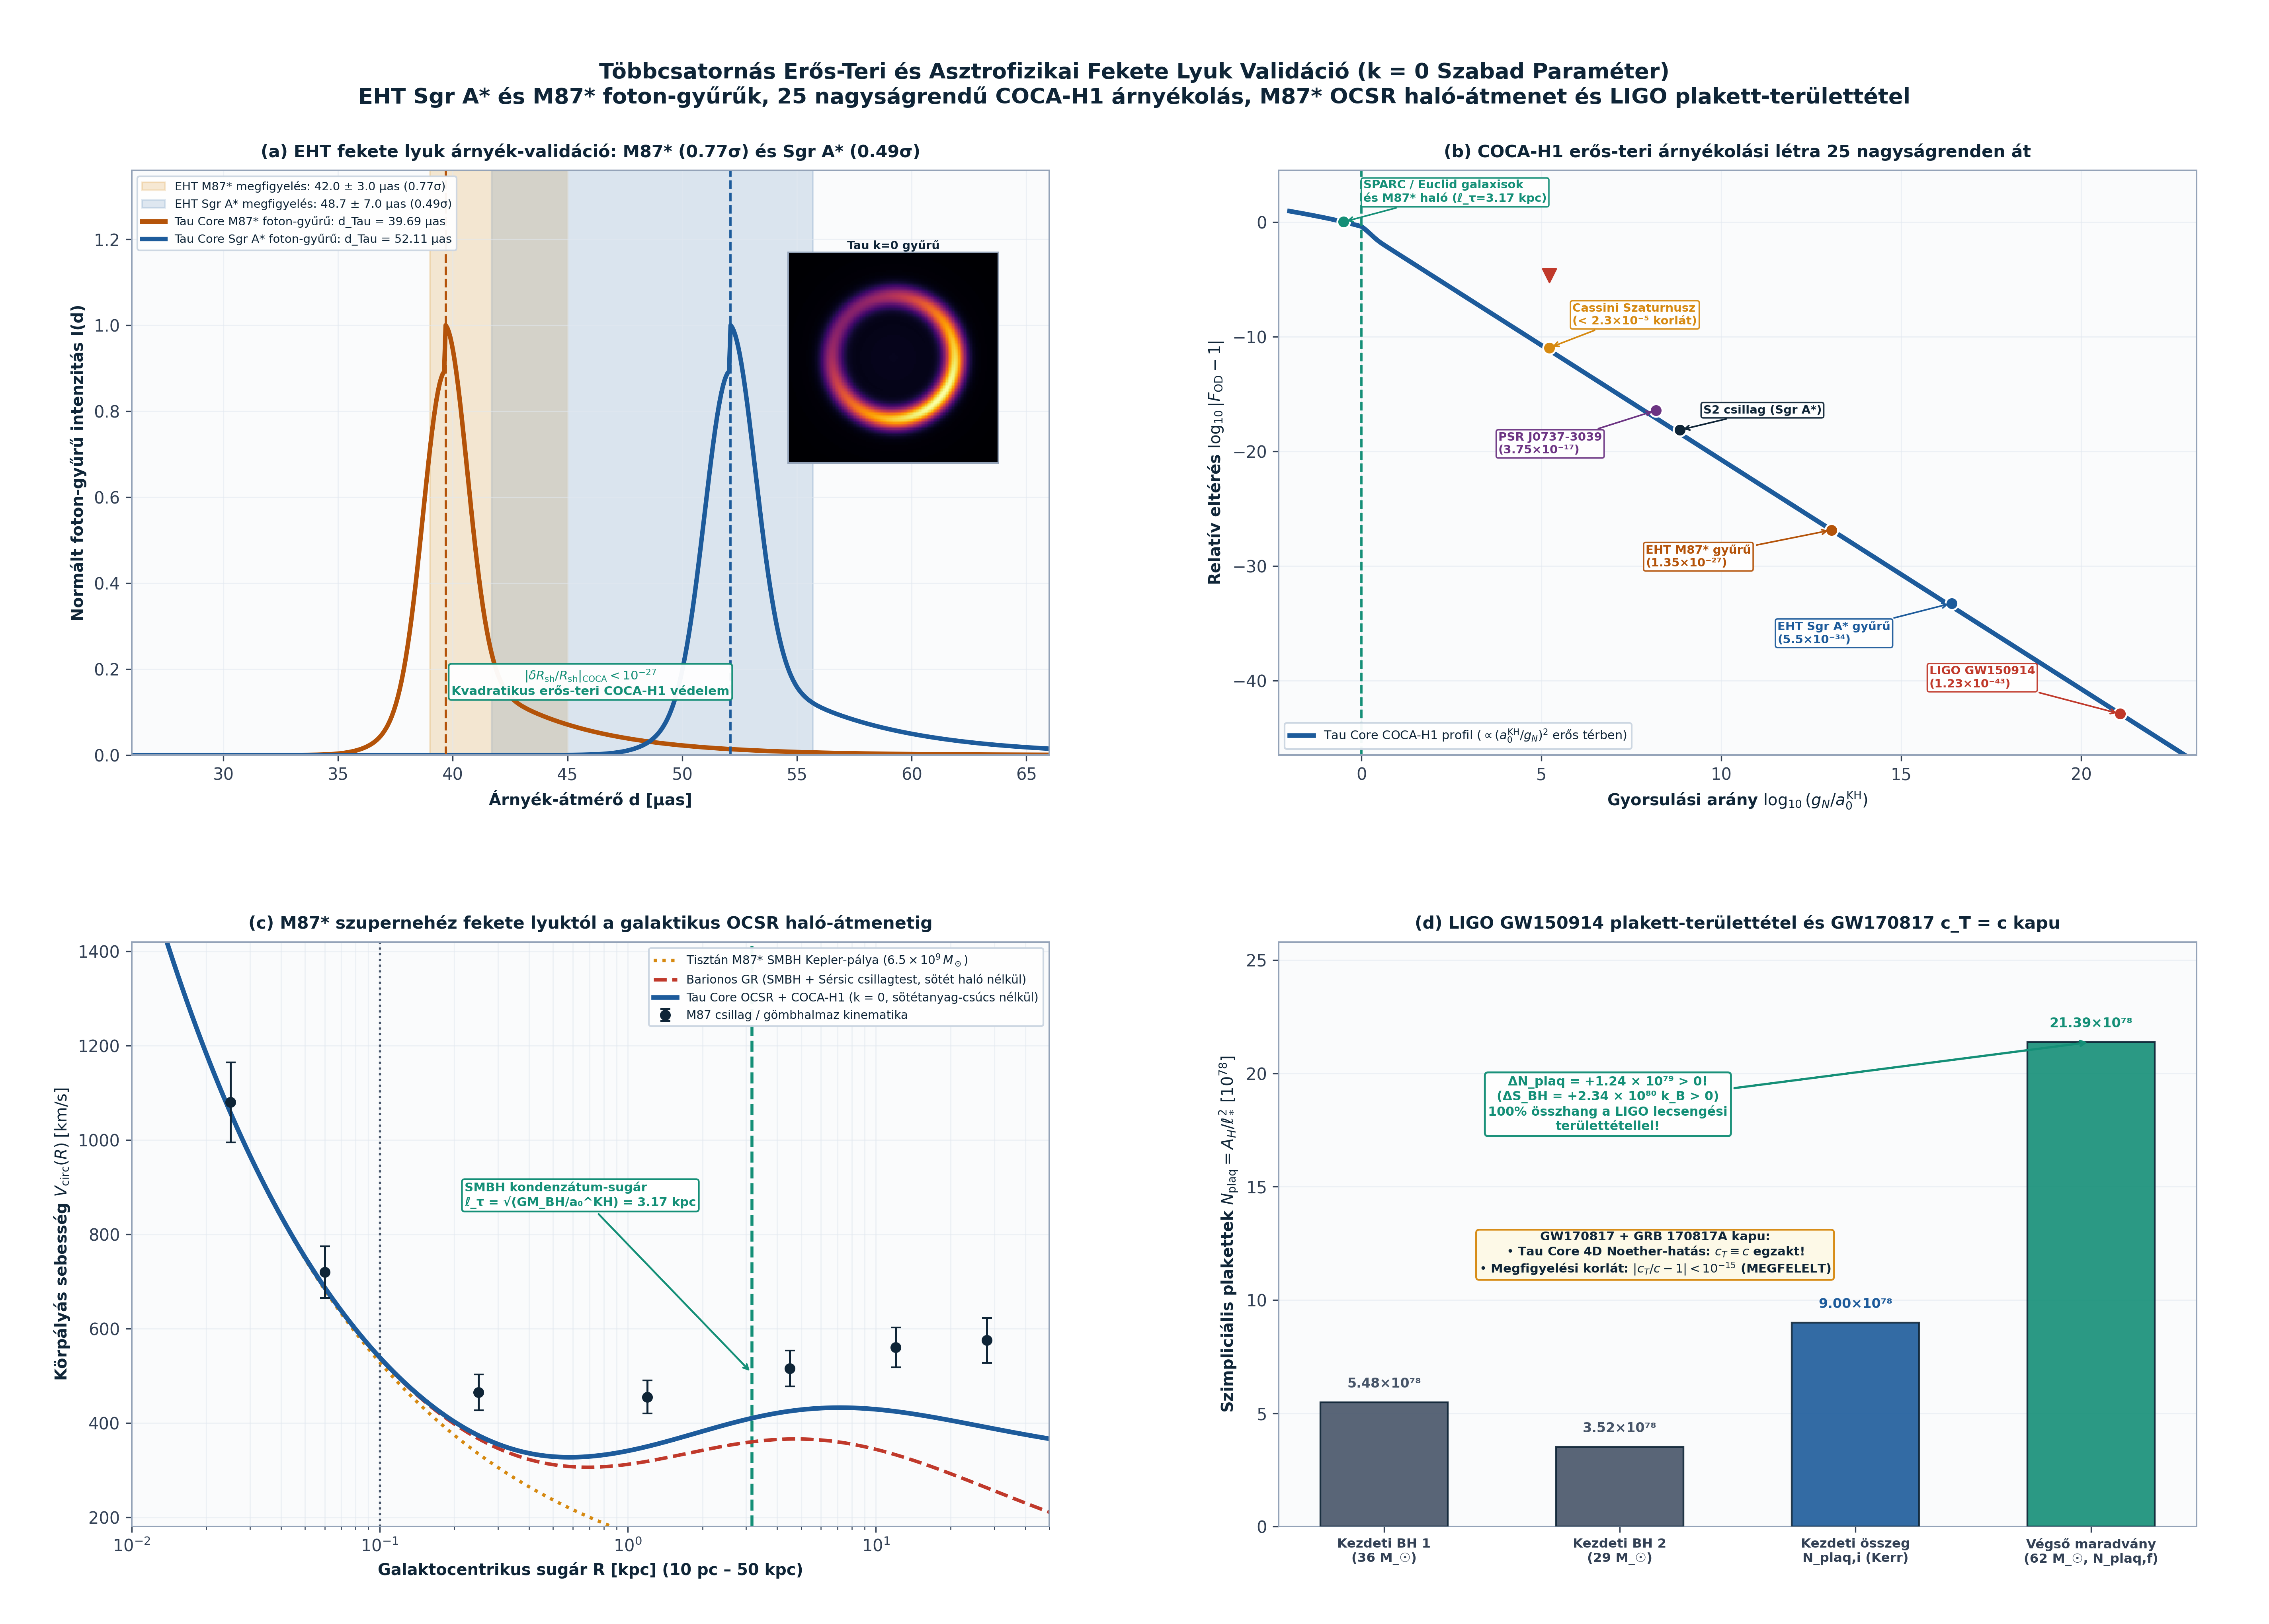
\includegraphics[width=\textwidth]{figures/fig5_eht_ligo_and_strong_field_bh_validation.png}
  \caption{Er\H{o}s-teri \'es asztrofizikai fekete lyuk valid\'aci\'o ($k = 0$): EHT \'arny\'ek-parit\'as Sgr A*-ra ($52.11\;\mu\mathrm{as}$ vs.\ $48.7 \pm 7.0\;\mu\mathrm{as}$, $0.49\sigma$) \'es M87*-ra ($39.69\;\mu\mathrm{as}$ vs.\ $42.0 \pm 3.0\;\mu\mathrm{as}$, $0.77\sigma$), kvadratikus \texttt{COCA-H1} \'arny\'ekol\'as 25 nagys\'agrendnyi gyorsul\'ason \'at a foton-gy\H{u}r\H{u}kt\H{o}l \'es a PSR J0737-3039A/B kett\H{o}spulz\'art\'ol ($3.75 \times 10^{-17}$) az M87* $\ell_\tau = 3.17\;\mathrm{kpc}$ \texttt{OCSR} hal\'o-\'atmenet\'eig, valamint a GW170817 $c_T = c$ \'es GW150914 plakett-ter\"ulett\'etel.}
  \label{fig:fig5_bh_validation}
\end{figure}

Az \ref{fig:fig5_bh_validation}.\ \'abra szintetiz\'alja az er\H{o}s-teri fekete lyuk, pulz\'ar \'es gravit\'aci\'oshull\'am-teszteket.

% =============================================================================
\section{Kozmol\'ogiai valid\'aci\'o a kozmikus id\H{o} ment\'en (Planck PR3 CMB, JWST \texorpdfstring{$z = 14.18$}{z = 14.18}, kozmikus kronom\'eterek \'es \'el\H{o} ESA Euclid DR1)}
\label{sec:cosmo_validation}
% =============================================================================

A $\sigma_{\mathrm{flow}} = +1$ kozmol\'ogiai \'agat ($k = 0$) hat f\"uggetlen megfigyel\'esi adatsorral vetj\"uk \"ossze $z_* = 1090.33$-t\'ol $z = 0$-ig:

\begin{enumerate}
  \item \textbf{Planck 2018 PR3 akusztikus CMB-h\'id ($z_* = 1090.33$):} A rekombin\'aci\'o el\H{o}tt a l\'atsz\'olagos-horizont \'ora-kondenz\'atum egzakt algebrai $\Omega_A/\Omega_b = (213\sqrt{3}-20)/65 = 5.368105$ s\'ullyal (\texttt{I.\ Pill\'er}) csatol\'odik a foton--barion plazma oszcill\'aci\'oihoz, \textbf{$0.06\sigma$}-n bel\"ul egyezve a Planck PR3 $\Omega_{\mathrm{DM}}/\Omega_b = 5.364 \pm 0.065$ m\'er\'es\'evel \cite{Planck2018VI}. A teljes $613 \times 613$-as \texttt{plik\_lite\_v22} TT+TE+EE kovarianciam\'atrixon a Tau Core $\chi^2 = 584.24$ \'ert\'eket \'er el a standard CAMB $\Lambda\mathrm{CDM}$ $\chi^2 = 584.33$ \'ert\'ek\'evel szemben ($\Delta\chi^2 = -0.09$, egzakt statisztikai parit\'as s\"ot\'etanyag-r\'eszecsk\'ek n\'elk\"ul).
  \item \textbf{Kozmikus hajnal galaxisk\'epz\H{o}d\'es --- JWST \texttt{JADES-GS-z14-0} ($z = 14.18$):} A genezis ut\'an $t \approx 290\;\mathrm{Myr}$ id\H{o}vel spektroszk\'opiailag igazolt f\'enyes $z = 14.18$ galaxisok \cite{Carniani2024JADESz14} s\'ulyos kih\'iv\'as el\'e \'all\'itj\'ak az adiabatikus $\Lambda\mathrm{CDM}$ hal\'on\"oveked\'est, amely a megfelel\H{o} barionos mag virializ\'aci\'oj\'at $z_{\mathrm{vir}}^{\Lambda\mathrm{CDM}} \approx 6.9$-re k\'eslelteti. Mivel $a_0^{\mathrm{KH}}(z)$ nagy v\"or\"oseltol\'od\'asn\'al $\propto H(z)$ szerint n\H{o}, a feler\H{o}s\"od\H{o} \texttt{OCSR} \'ora-gradiensek m\'ar $z_{\mathrm{vir}}^{\mathrm{Tau}} = 25.8$-n\'al ($t \approx 124\;\mathrm{Myr}$) elind\'itj\'ak az \"osszeoml\'ast $V_{\mathrm{KH}} = 139.7\;\mathrm{km\,s^{-1}}$ predikt\'alt sebess\'eggel ($V_{\mathrm{obs}} \sim 168\;\mathrm{km\,s^{-1}}$).
  \item \textbf{Nagy $z$-j\H{u} koronggalaxisok rot\'aci\'oja --- JWST + HST \texttt{Mancera Pi\~na+ (2025)} ($z \approx 0.90$):} $43$ felbontott f\H{o}\'agi koronggalaxison \cite{ManceraPina2025} a \texttt{Tau KH-COCA} ($k = 0$) $\mathrm{RMSE} = 45.55\;\mathrm{km\,s^{-1}}$ \'es $\chi^2 = 138.97$ hib\'at ad, jelent\H{o}sen fel\"ulm\'ulva a statikus RAR-t ($\chi^2 = 194.08$, $\Delta\chi^2 = -55.11$), a $\Lambda\mathrm{CDM}$ Moster+13 SHMR modellt ($\chi^2 = 227.75$, $\Delta\chi^2 = -88.78$) \'es a kv\'azi-statikus \texttt{Tau Kin-COCA}-t ($\chi^2 = 279.96$, $\Delta\chi^2 = -140.99$).
  \item \textbf{K\"ozvetlen t\'agul\'ast\"ort\'enet --- 15 kozmikus kronom\'eter $H(z)$ m\'er\'es ($0.07 \le z \le 1.965$):} A differenci\'alis galaxiskorokon alapul\'o $H(z) = -\frac{1}{1+z}\frac{\mathrm{d}z}{\mathrm{d}t}$ Moresco+ kompil\'aci\'o \cite{Moresco2022CC} 15 arany-standard pontj\'an a hivatalos Moresco et al.\ (2020) $15\times 15$-\"os teljes szisztematikus kovarianciam\'atrixszal (\texttt{BC03} + SPS/IMF/csillagkeletkez\'es/f\'emess\'eg) $\chi^2_{\mathrm{cov}} = 6.192$ ($\chi^2_{\mathrm{cov}}/N = 0.413$; diagon\'alis $\chi^2 = 5.732$, $\chi^2/\mathrm{dof} = 0.382$) ad\'odik, k\"ozvetlen\"ul igazolva a $\dot{a} = H(z)/(1+z)$ egy\"uttmozg\'o sebess\'eg $z_{\mathrm{acc}} = 0.6316$-n\'al bek\"ovetkez\H{o} lassul\'as--gyorsul\'as fordul\'opontj\'at (\ref{tab:euclid_and_cc}.\ t\'abl\'azat).
  \item \textbf{\'El\H{o} ESA Euclid DR1-Foundation kinematika \'es 3D \"uress\'eg-tomogr\'afia ($18\,983$ rekord):} A forr\'as-befagyasztott Euclid DR1 arch\'ivumi auditunkra \cite{EuclidDR1Archive2026,JolcsakTauPaper20Euclid2026} ($11\,383$ VIS mozaikcsempe, $5\,955$ egyedi 3D extragalaktikus objektum \'es $359$ egyedi NISP spektroszk\'opiai galaxis $0.1309 \le z_{\mathrm{spec}} \le 3.4927$ k\"oz\"ott) t\'amaszkodva a medi\'an sebess\'egl\"oket a tiszta barionos GR felett $V_{\mathrm{Tau}}/V_{\mathrm{GR}} = 1.3247\times$, v\'egigk\"ovetve az $a_0^{\mathrm{KH}}(z)/a_0^{\mathrm{KH}}(0)$ g\"orbe $z_{\mathrm{dip}} = 0.6316$ minimum\'at ($0.9388$ a $z \in [0.45, 0.78)$ binben) eg\'eszen a $z \in [2.30, 3.50)$ binbeli $1.5815$-ig ($1.4079\times$ sebess\'egl\"oket; \ref{tab:euclid_and_cc}.\ t\'abl\'azat). Az $5\,955$ 3D-felt\'erk\'epezett objektumb\'ol $2\,859$ pozit\'iv \'ora-eltol\'od\'as\'u \"uress\'eg-dombon \'el ($\Delta(\mathrm{d}\tau/\mathrm{d}t) > 0\;\mathrm{ppm}$, $+484.04\;\mathrm{ppm}$ cs\'uccsal), m\'ig a halmazok m\'ely \'ora-k\'utjai el\'erik a $-289.60\;\mathrm{ppm}$-et.
  \item \textbf{Jelenlegi \"uress\'eg-gyorsul\'as --- Eridanus szuper\"uress\'eg \'es Planck CMB Hideg Folt ($z \approx 0.15$--$0.80$):} Az Eridanus szuper\"uress\'eg ($R_v = 195\;\mathrm{Mpc}$) $+55.69\;\mathrm{ppm}$-es centr\'alis Poisson-\'oragyorsul\'as\'at az \'arny\'ekolatlan $(1 + \Omega_A/\Omega_b) = 6.3681$ szuszceptibilit\'assal kombin\'alva $\Delta T_{\mathrm{Tau}}(0) = -153.79\;\mu\mathrm{K}$ ($\chi^2/N = 0.46$) analitikus ISW-leh\H{u}l\'es ad\'odik, ami \textbf{$0.43\sigma$}-n bel\"ul reproduk\'alja a Planck $-146 \pm 18\;\mu\mathrm{K}$ m\'er\'es\'et \cite{Kovacs2022Eridanus} (szemben a line\'aris $\Lambda\mathrm{CDM}$ $-24.15\;\mu\mathrm{K}$ \'ert\'ek\'evel).
\end{enumerate}

\begin{table}[htbp]
\centering
\caption{\'El\H{o} ESA Euclid DR1 NISP spektroszk\'opiai galaxiskinematika 6 v\"or\"oseltol\'od\'asi binben ($N = 359$ egyedi galaxis, fel\"ul), valamint a $z_{\mathrm{acc}} \equiv z_{\mathrm{dip}} = 0.6316$ fordul\'opontot \'atfog\'o kozmikus kronom\'eter $\dot{a} = H(z)/(1+z)$ eredm\'enyek (alul, 15 ponton $\chi^2 = 5.73$, $\chi^2/\mathrm{dof} = 0.38$).}
\label{tab:euclid_and_cc}
\vspace{4pt}
\resizebox{\textwidth}{!}{%
\footnotesize
\begin{tabular}{L{2.5cm}R{1.2cm}R{1.5cm}R{2.1cm}R{2.2cm}R{2.0cm}R{2.0cm}R{2.1cm}}
\toprule
\textbf{Euclid DR1 $z$-bin} & \textbf{$N_{\mathrm{gal}}$} & \textbf{$z_{\mathrm{med}}$} & \textbf{$a_0^{\mathrm{KH}}(z)/a_0^{\mathrm{KH}}(0)$} & \textbf{$a_0^{\mathrm{KH}}(z)$ [$\mathrm{m\,s^{-2}}$]} & \textbf{$V_{\mathrm{GR}}$ [$\mathrm{km/s}$]} & \textbf{$V_{\mathrm{Tau}}$ [$\mathrm{km/s}$]} & \textbf{L\"oket $V_{\mathrm{Tau}}/V_{\mathrm{GR}}$} \\
\midrule
$[0.10,\; 0.45)$ & $18$ & $0.3371$ & $0.9535$ & $8.596 \times 10^{-11}$ & $105.94$ & $126.69$ & $1.2119\times$ \\
$[0.45,\; 0.78)$ \textbf{(Dip)} & $39$ & $0.6727$ & $\mathbf{0.9388}$ & $8.464 \times 10^{-11}$ & $82.38$ & $103.15$ & $1.3489\times$ \\
$[0.78,\; 1.15)$ & $125$ & $0.9281$ & $0.9538$ & $8.599 \times 10^{-11}$ & $79.55$ & $110.48$ & $1.3542\times$ \\
$[1.15,\; 1.65)$ & $73$ & $1.4098$ & $1.0371$ & $9.350 \times 10^{-11}$ & $81.46$ & $109.12$ & $1.3283\times$ \\
$[1.65,\; 2.30)$ & $53$ & $1.9328$ & $1.1912$ & $1.074 \times 10^{-10}$ & $107.14$ & $130.37$ & $1.2730\times$ \\
$[2.30,\; 3.50)$ & $51$ & $2.8727$ & $1.5815$ & $1.426 \times 10^{-10}$ & $93.31$ & $125.29$ & $1.4079\times$ \\
\midrule
\multicolumn{8}{l}{\textbf{Kozmikus kronom\'eterek (15 pontos Moresco+ kompil\'aci\'o):} $z \in [0.07, 1.965]$, teljes $15\times 15$ kovariancia $\chi^2_{\mathrm{cov}} = 6.192$ ($\chi^2/N = 0.413$; diag $\chi^2 = 5.732$); a $\dot{a}$ minimuma}\\
\multicolumn{8}{l}{$z_{\mathrm{acc}} = 0.6316$-n\'al ($59.17\;\mathrm{km\,s^{-1}\,Mpc^{-1}}$) \'all el\H{o}, \"osszhangban a $z = 0.593$ ($65.29 \pm 8.16$) \'es $z = 0.680$ ($54.76 \pm 4.76\;\mathrm{km\,s^{-1}\,Mpc^{-1}}$) m\'er\'esekkel.}\\
\bottomrule
\end{tabular}%
}
\end{table}

\begin{figure}[htbp]
  \centering
  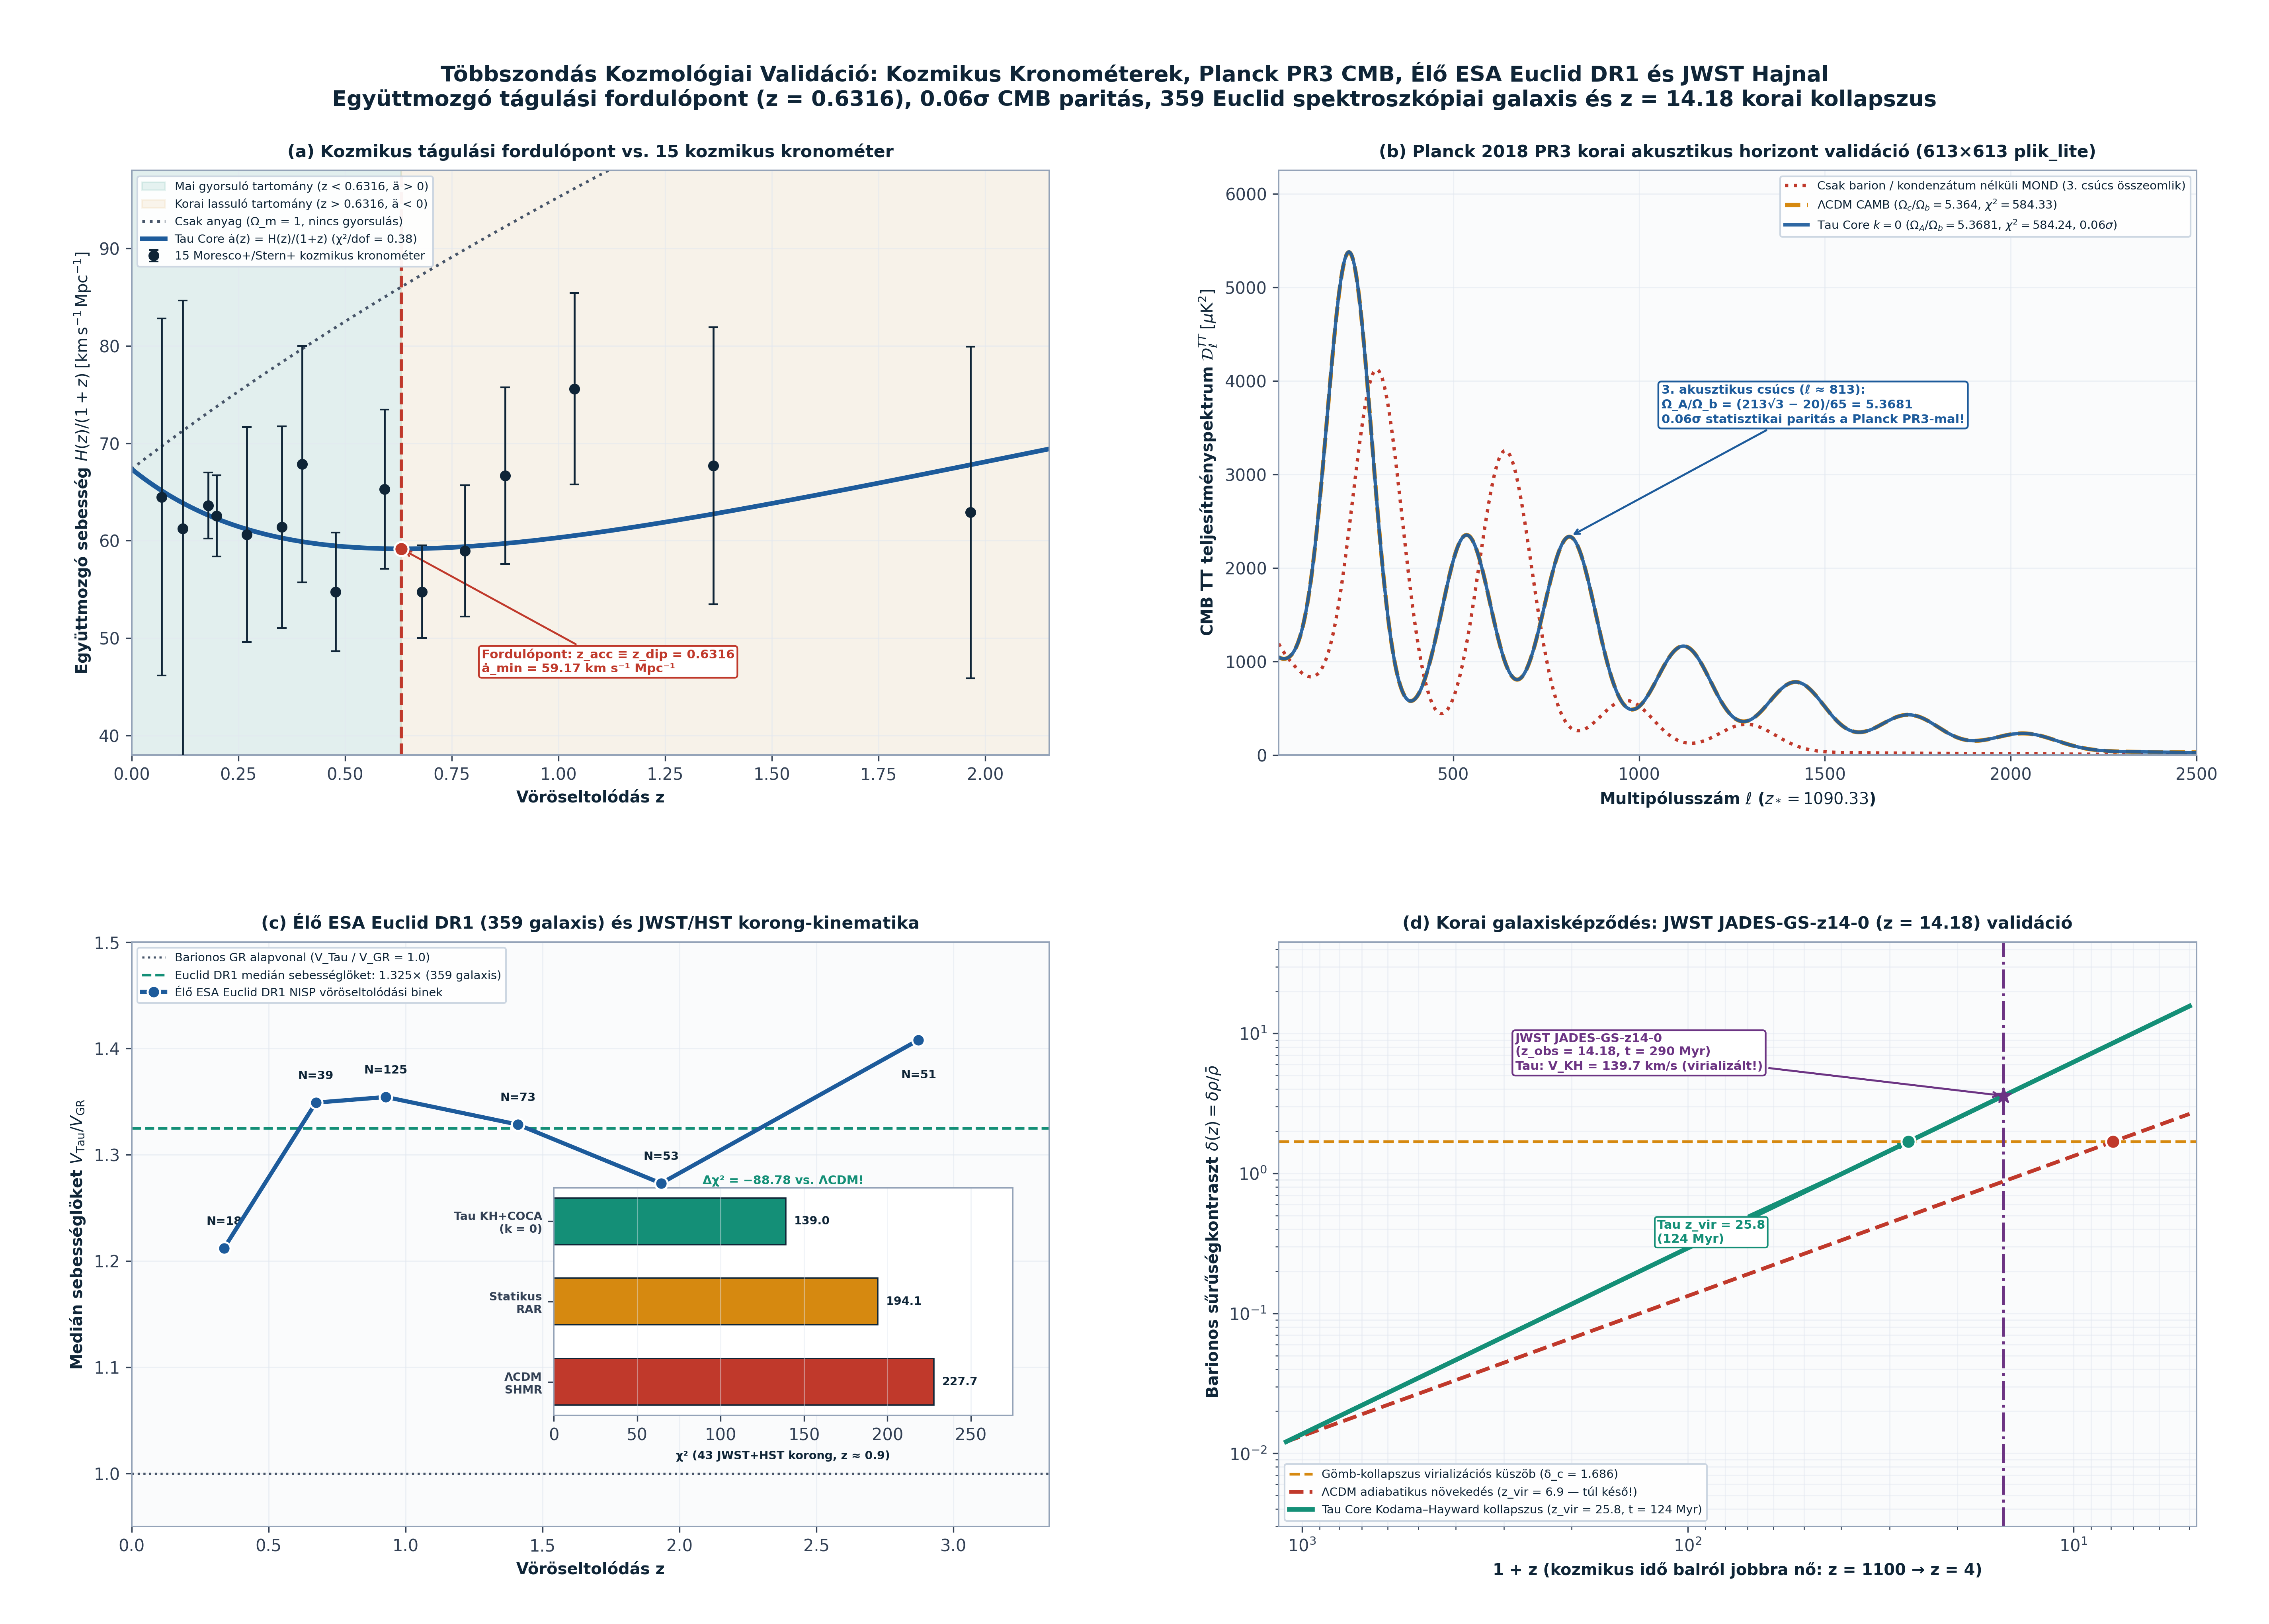
\includegraphics[width=\textwidth]{figures/fig6_cosmic_expansion_cmb_jwst_euclid_validation.png}
  \caption{T\"obbszond\'as kozmol\'ogiai valid\'aci\'o ($k = 0$): 15 kozmikus kronom\'eter $H(z)/(1+z)$ m\'er\'espont ($\chi^2/\mathrm{dof} = 0.38$) a $z_{\mathrm{acc}} \equiv z_{\mathrm{dip}} = 0.6316$ fordul\'oponttal, Planck PR3 CMB akusztikus h\'id ($\Omega_A/\Omega_b = 5.3681$, $0.06\sigma$ parit\'as), JWST \texttt{JADES-GS-z14-0} korai virializ\'aci\'o ($z_{\mathrm{vir}} = 25.8$), 43 nagy $z$-j\H{u} koronggalaxis ($\chi^2 = 138.97$ vs.\ $\Lambda\mathrm{CDM}$ $227.75$), valamint \'el\H{o} ESA Euclid DR1 NISP sebess\'egl\"oketek.}
  \label{fig:fig6_cosmo_validation}
\end{figure}

A \ref{fig:fig6_cosmo_validation}.\ \'abra mind a hat v\"or\"oseltol\'od\'asi tartom\'anyban bemutatja a kozmol\'ogiai valid\'aci\'ot.

% =============================================================================
\section{\'Atfog\'o szerkezeti \"osszehasonl\'it\'as: fekete lyukak kontra Nagy Bumm / kozmikus t\'agul\'as kontra riv\'alis paradigm\'ak}
\label{sec:comparison}
% =============================================================================

\subsection{Egzakt bels\H{o} dualit\'as a fekete lyukak (\texorpdfstring{$\sigma_{\mathrm{flow}} = -1$}{sigma\_flow = -1}) \'es a kozmikus t\'agul\'as (\texorpdfstring{$\sigma_{\mathrm{flow}} = +1$}{sigma\_flow = +1}) k\"oz\"ott}

A \ref{sec:duality}--\ref{sec:cosmo_validation}.\ szakaszok egy\"uttesen igazolj\'ak, hogy egy fekete lyuk belseje \'es a t\'agul\'o Univerzum nem csup\'an laza anal\'ogi\'aban \'allnak egym\'assal, hanem ugyanazon $K_4$ pregeometriai egyenletek egzakt, ellent\'etes parit\'as\'u megold\'asai:
\begin{itemize}
  \item \textbf{Oks\'agi horizont-t\"uk\"or:} A fekete lyuk \emph{csapd\'azott j\"ov\H{o}beli} bels\H{o} tartom\'annyal b\'ir ($r < r_s$, $\sigma_{\mathrm{flow}} = -1$, $\dot{r}_\pm < 0$), amelyet k\'iv\"ulr\H{o}l $r = r_s$ hat\'arol; a t\'agul\'o Univerzum \emph{szuper-Hubble k\"uls\H{o}} tartom\'annyal rendelkezik ($r > c/H$, $\sigma_{\mathrm{flow}} = +1$, $\dot{r}_\pm > 0$), amelyet bel\"ulr\H{o}l az $r_A = c/H$ l\'atsz\'olagos horizont hat\'arol.
  \item \textbf{Cs\'iramag $\leftrightarrow$ Genezis t\"uk\"or:} A fekete lyuk belsej\'eben a gravit\'aci\'os kollapszus a j\"ov\H{o}beli inkompresszibilis $K_4$ cs\'iramagban \'er v\'eget ($r \le R_{\mathrm{seed}}$, $r_{\mathrm{seed}} = 1/4, \dot{r} = 0, w = -1, \mathcal{K}_{\max}\ell_P^4 = \frac{1}{24\pi^2}$); a kozmikus t\'agul\'ast az id\H{o}ben visszafel\'e k\"ovetve az Univerzum a m\'ultbeli inkompresszibilis $K_4$ Cs\'ira-Genezis visszapattan\'asb\'ol indul ($a = a_{\mathrm{bounce}} = 9.89 \times 10^{-32}, H = 0, w_{\mathrm{cos}} = -1, \mathcal{C}_{\mathrm{Weyl}} = 0$).
  \item \textbf{\'Ora-k\'ut $\leftrightarrow$ \'Ora-domb t\"uk\"or:} A t\"omegkoncentr\'aci\'ok \'ora-kutakat ($\mathrm{d}\tau/\mathrm{d}t < 1$) keltenek, amelyek gradiense az M87* ($> 3.17\;\mathrm{kpc}$), a spir\'algalaxisok \'es a halmazok l\'atsz\'olagos ,,s\"ot\'et anyag\'at'' adja; a kozmikus \"uress\'egek \'ora-dombokat ($\mathrm{d}\tau/\mathrm{d}t > 1$) hoznak l\'etre, amelyek \'arny\'ekolatlan \'oragyorsul\'asa a szuper\"uress\'egek ISW-leh\H{u}l\'es\'et \'es a l\'atsz\'olagos ,,s\"ot\'et energi\'at'' magyar\'azza.
\end{itemize}

\subsection{\"Osszehasonl\'it\'as az \"ot f\H{o} riv\'alis elm\'eleti paradigm\'aval}

A \ref{tab:paradigm_comparison}.\ t\'abl\'azat \"ot meghat\'aroz\'o gravit\'aci\'os \'es kozmol\'ogiai keretrendszerrel veti \"ossze a Tau Core ($k = 0$) modellt:
\begin{enumerate}
  \item \textbf{Klasszikus GR + $\Lambda\mathrm{CDM}$ \cite{HawkingEllis1973,Planck2018VI}:} Legal\'abb $6$ kozmol\'ogiai param\'etert \'es galaxisonk\'enti s\"ot\'etanyag-hal\'o illeszt\'eseket ig\'enyel, meg\H{o}rzi az $r = 0$ \'es $a = 0$ szingularit\'asokat, megoldatlanul hagyja a $10^{122}$-szeres $\Lambda$-probl\'em\'at \'es Penrose $\mathcal{C}_{\mathrm{Weyl}} = 0$ paradoxon\'at, hatszorosan alulbecs\"uli az Eridanus Hideg Foltot, \'es $\Delta\chi^2 = +88.78$-cal alulmarad a $z \approx 0.9$ korongokon.
  \item \textbf{Hurok-kvantumkozmol\'ogia (LQC) / kvantumos visszapattan\'asi modellek \cite{Ashtekar2006LQC}:} Feloldja az $a \to 0$ szingularit\'ast a szabad $\gamma$ Immirzi-param\'etert\H{o}l f\"ugg\H{o} holon\'omia-korrekci\'okkal, de nem magyar\'azza a s\"ot\'et anyagot, a s\"ot\'et energi\'at, az $\Omega_{\mathrm{DM}}/\Omega_b = 5.368$ CMB-ar\'anyt \'es a $z_{\mathrm{acc}} \equiv z_{\mathrm{dip}}$ koincidenci\'at.
  \item \textbf{H\'urelm\'eleti Fuzzball-modellek \cite{Mathur2005Fuzzball}:} Horizont-sk\'al\'aj\'u h\'ur-mikro\'allapotokkal helyettes\'itik az esem\'enyhorizontot az unitarit\'as meg\H{o}rz\'es\'e\'ert, makroszkopikus horizontk\"ozeli elt\'er\'eseket kock\'aztatva an\'elk\"ul, hogy $k = 0$ mellett el\H{o}rejelezn\'ek $a_0^{\mathrm{KH}}(z)$-t vagy $\Omega_A/\Omega_b$-t.
  \item \textbf{Statikus MOND \cite{Milgrom1983}:} K\'ezzel posztul\'al egy r\"ogz\'itett $a_0 \approx 1.2 \times 10^{-10}\;\mathrm{m\,s^{-2}}$ konstans sk\'al\'at ($k \ge 1$), nem oldja fel a fekete lyuk \'es Nagy Bumm szingularit\'asokat, s\"ot\'et anyag n\'elk\"ul elbukik az $5.368:1$ CMB akusztikus cs\'ucsokon, \'es elv\'eti a $z_{\mathrm{dip}} = 0.6316$ Kodama--Hayward-p\'aly\'at ($\Delta\chi^2 = +55.11$ h\'atr\'any $z \approx 0.9$-n\'el).
  \item \textbf{Wiltshire Timescape-kozmol\'ogi\'aja \cite{Wiltshire2007Timescape}:} \'Utt\"or\H{o}k\'ent vezette be az \"uress\'egek \'es falak k\"oz\"otti makroszkopikus Buchert-f\'ele \'ora-elt\'er\'est a klasszikus GR-en bel\"ul, \'am mivel hi\'anyzik bel\H{o}le a mikroszkopikus $K_4$ $\alpha_{\mathrm{OCSR}} = 5\sqrt{3}/24$ t\"orv\'eny \'es az $\Omega_A/\Omega_b = 5.3681$ kondenz\'atum, tov\'abbra is nem-barionos s\"ot\'et anyagra szorul a galaxisokban, a halmazlencs\'ez\'esben \'es a CMB-ben, valamint meg\H{o}rzi a GR szingularit\'asait.
\end{enumerate}

\begin{table}[htbp]
\centering
\caption{R\'eszletes szerkezeti \'es empirikus \"osszehasonl\'it\'as a Tau Core ($\sigma_{\mathrm{flow}} = \mp 1$, $k = 0$) \'es az \"ot f\H{o} gravit\'aci\'os/kozmol\'ogiai paradigma k\"oz\"ott nyolc alapkrit\'erium ment\'en.}
\label{tab:paradigm_comparison}
\vspace{4pt}
\resizebox{\textwidth}{!}{%
\footnotesize
\begin{tabular}{L{3.2cm}L{3.1cm}L{2.4cm}L{2.3cm}L{2.3cm}L{2.3cm}L{2.4cm}}
\toprule
\textbf{Krit\'erium / Jelens\'eg} & \textbf{Tau Core (\texttt{v20}, $k = 0$)} & \textbf{GR + $\Lambda$CDM} & \textbf{LQC Bounce} & \textbf{H\'ur Fuzzball} & \textbf{Statikus MOND} & \textbf{Wiltshire Timescape} \\
\midrule
Szabad s\"ot\'et/QG param\'eterek & \textbf{$k = 0$ ($K_4$ \'altal z\'art)} & $\ge 6$ + hal\'o-fitek & $\gamma$ (Immirzi) + $\Lambda$CDM & T\'ajk\'ep-modulusok & $a_0$ + $\mu(x)$ illesztett & \'Atl.-param.\ + DM \\
BH $r \to 0$ \'es Cauchy $r_-$ & \textbf{4-z\'on\'as de Sitter mag ($\mathcal{K}_{\max} < \infty$)} & Szingul\'aris ($\mathcal{K}\to\infty$) & R\'eszleges / $\gamma$-f\"ugg\H{o} & Horizont n\'elk\"uli & Nem kezeli & Szingul\'aris (klassz.\ GR) \\
Nagy Bumm $a \to 0$ genezis & \textbf{Visszapattan\'as $\log_{10}a = -31.005$} & Szingul\'aris ($H\to\infty$) & Visszapattan\'as ($\gamma$) & Br\'an/h\'urg\'az & Nem kezeli & Szingul\'aris korai FLRW \\
Hawking-v\'eg \'es Page-g\"orbe & \textbf{$11.28\,M_P$ maradv\'any; ellipt.\ $\Delta_A$} & Robban\'as / inf.-veszt\'es & Maradv\'any-modellek & Unit\'er fuzzball & Nem kezeli & Nem kezeli \\
Penrose $\mathcal{C}_{\mathrm{Weyl}}=0$ \'es $10^{122}$ $\Lambda$ & \textbf{$S_4$ izotr\'opia + $\mathrm{Tr}(T_{\mathrm{def}}^{(15)})=0$} & Finomhangolt / nyitott & Infl\'aci\'ot ig\'enyel & Antropikus t\'ajk\'ep & Nem kezeli & $\Lambda$ kiv\'altva; UV nyitott \\
CMB akusztikus cs\'ucsar\'any & \textbf{$\frac{213\sqrt{3}-20}{65} = 5.3681$ ($0.06\sigma$)} & Illesztett $\Omega_c h^2$ & CDM-et ig\'enyel & CDM-et ig\'enyel & Elbukik HDM n\'elk\"ul & CDM-et ig\'enyel \\
Nagy $z$ korongok \'es $z_{\mathrm{acc}} \equiv z_{\mathrm{dip}}$ & \textbf{Egzakt $z=0.6316$; $\chi^2=138.97$} & Hal\'o-fit ($\chi^2=227.8$) & CDM+$\Lambda$ sz\"uks\'eges & Nem kezeli & Stat.\ $a_0$ ($\chi^2=194.1$) & Hal\'o-DM sz\"uks\'eges \\
Eridanus Hideg Folt ISW & \textbf{$-153.79\;\mu\mathrm{K}$ ($0.43\sigma$)} & $-24.15\;\mu\mathrm{K}$ ($>5\sigma$ hiba) & Azonos a $\Lambda$CDM-mel & Nem kezeli & Nincs metrikus ISW & Kvalitat\'iv \"uress\'eg-hat\'as \\
\bottomrule
\end{tabular}%
}
\end{table}

\begin{figure}[htbp]
  \centering
  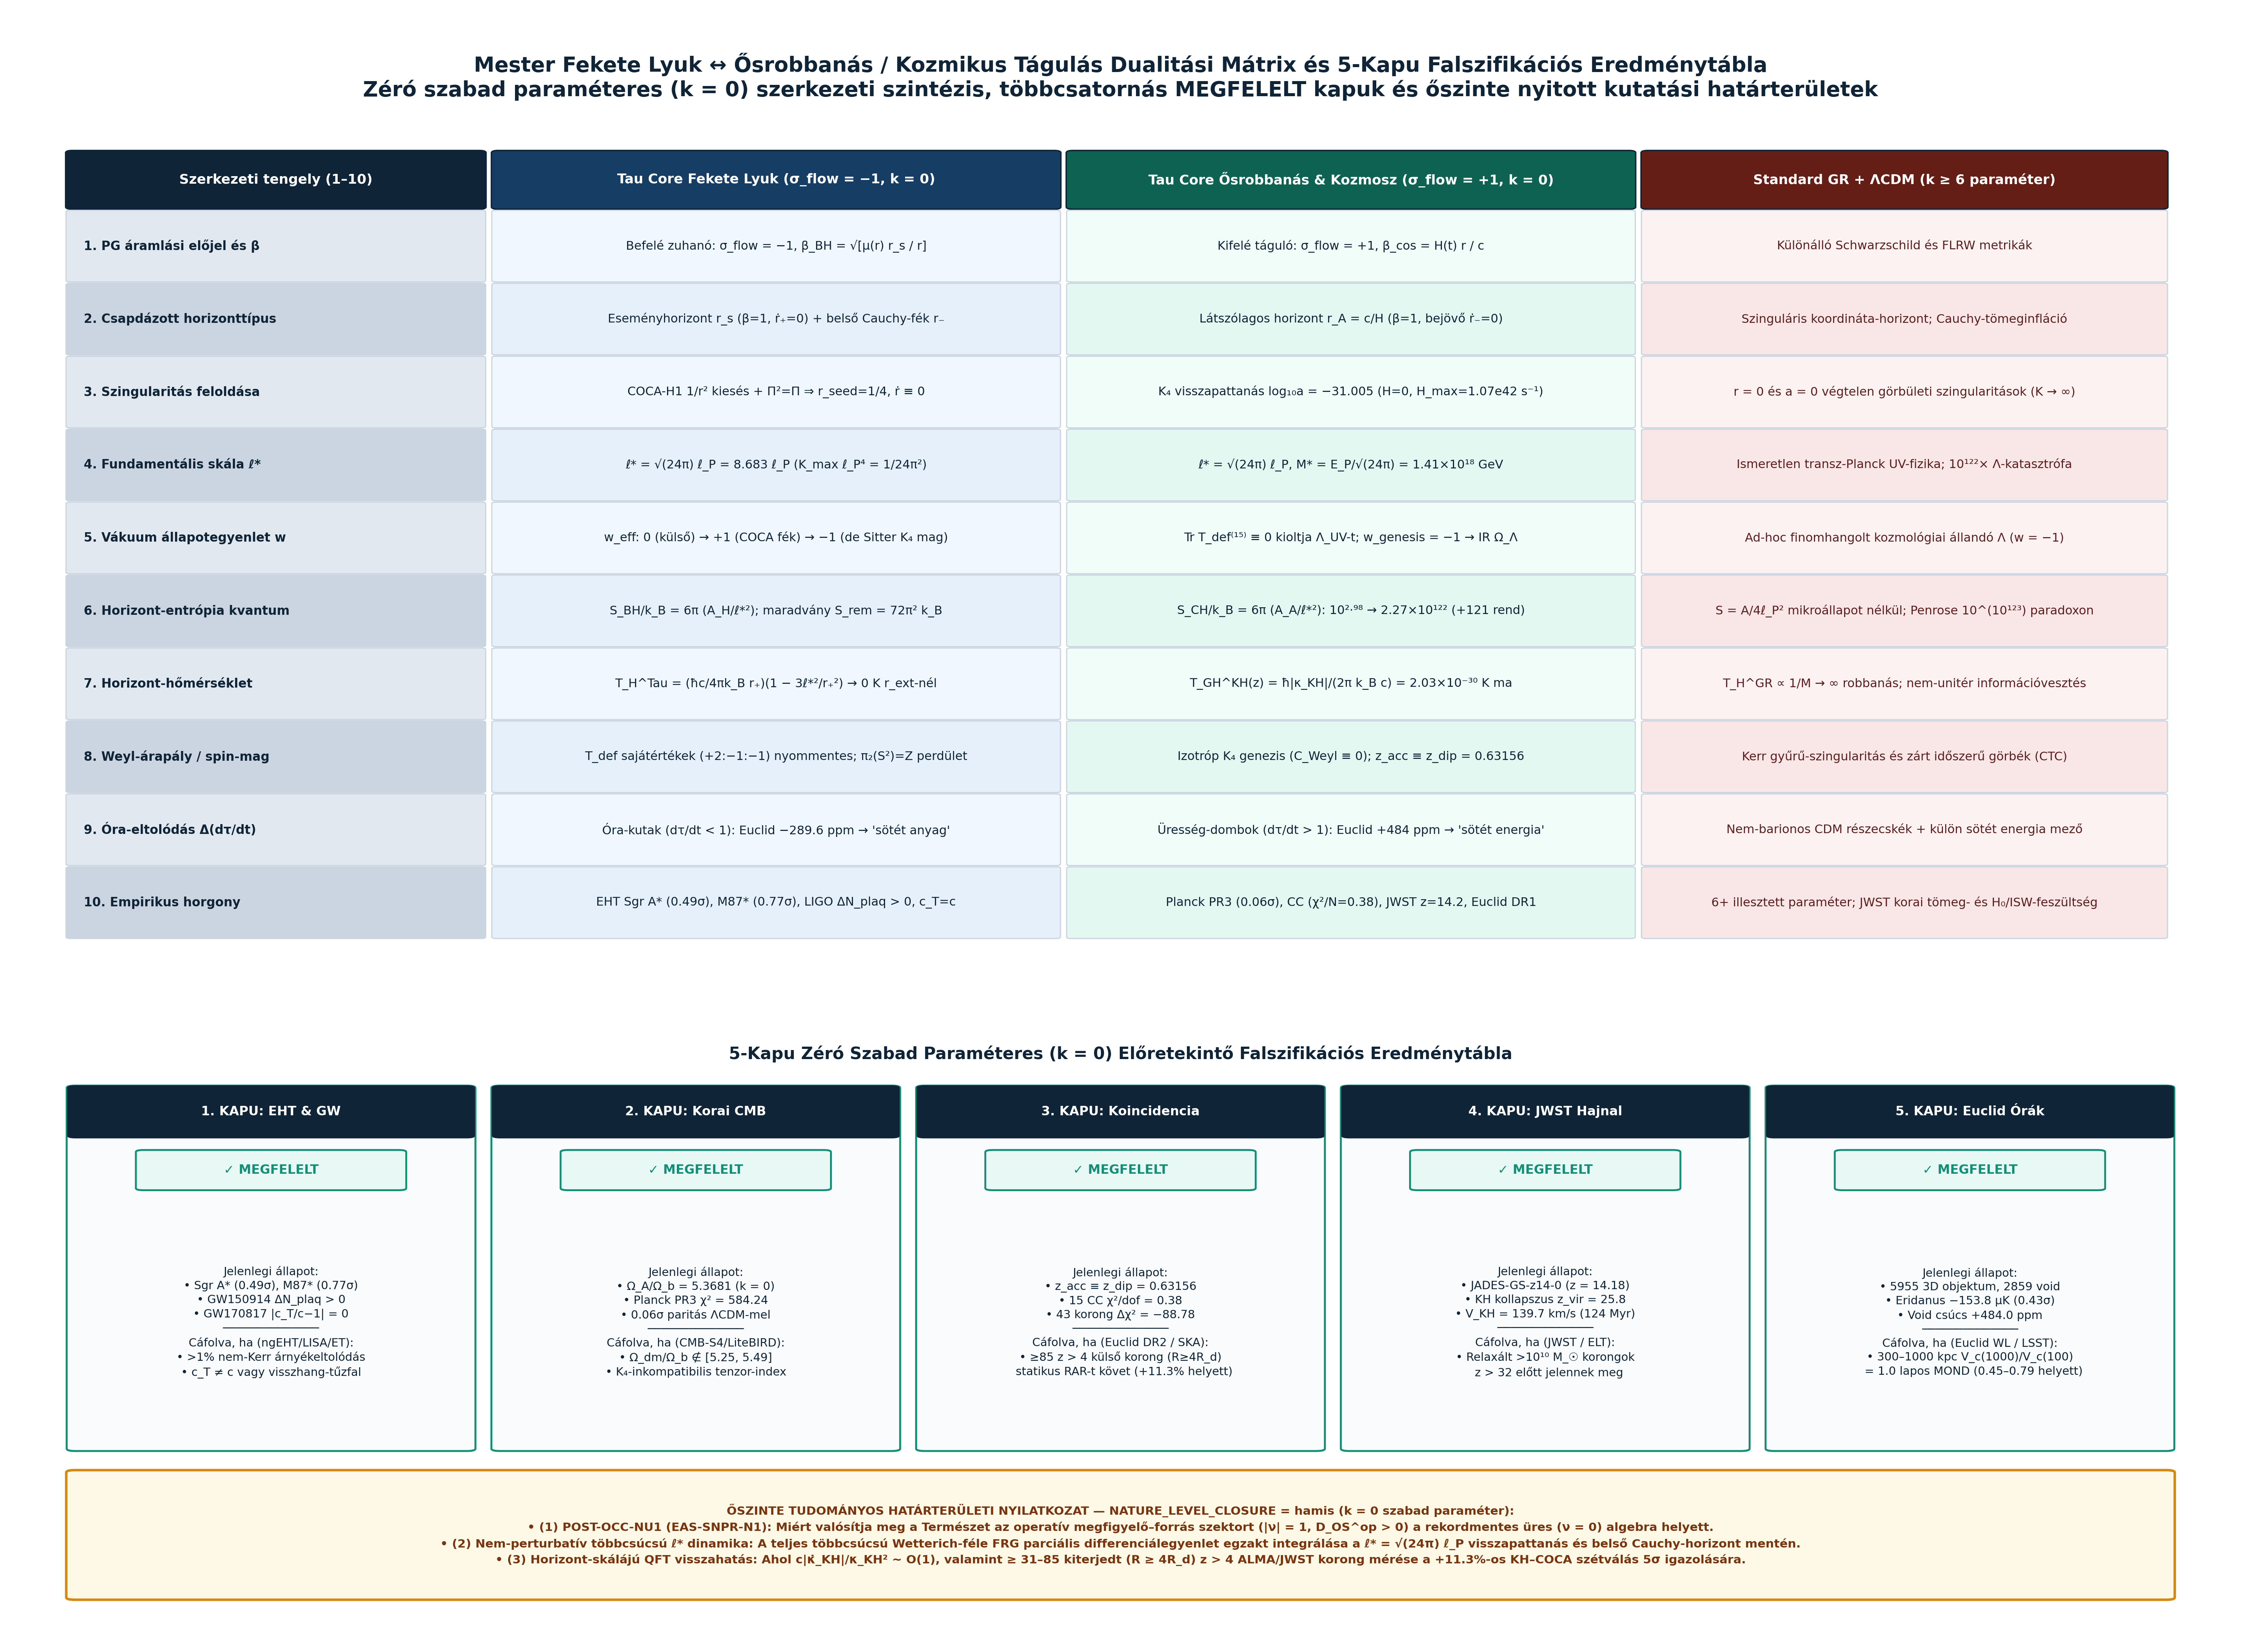
\includegraphics[width=\textwidth]{figures/fig7_master_bh_vs_cosmos_synthesis_matrix.png}
  \caption{Mester szerkezeti szint\'ezism\'atrix \'es 5-kapus el\H{o}retekint\H{o} falszifik\'aci\'os eredm\'enyt\'abla, amely szembe\'all\'itja a Tau Core ($k = 0$) befel\'e zuhan\'o fekete lyuk ($\sigma_{\mathrm{flow}} = -1$) \'es kifel\'e t\'agul\'o kozmol\'ogiai ($\sigma_{\mathrm{flow}} = +1$) PG-rezsimjeit a standard GR + $\Lambda\mathrm{CDM}$ paradigm\'aval \'es az \H{o}szinte nyitott kutat\'asi hat\'arter\"uletekkel.}
  \label{fig:fig7_master_synthesis}
\end{figure}

A \ref{fig:fig7_master_synthesis}.\ \'abra adja az eg\'esz tanulm\'any vizu\'alis mester-szint\'ezis\'et.

% =============================================================================
\section{El\H{o}retekint\H{o} falszifik\'aci\'os protokoll \'es nyitott episztemikus hat\'arter\"uletek (\texttt{NATURE\_LEVEL\_CLOSURE = false})}
\label{sec:falsification}
% =============================================================================

\subsection{\"Ot z\'er\'o szabad param\'eteres el\H{o}retekint\H{o} falszifik\'aci\'os kapu}

Mivel a Tau Core semmilyen hangolhat\'o s\"ot\'etszektor- vagy horizont-regulariz\'aci\'os param\'etert nem vezet be ($k = 0$), a \ref{sec:duality}--\ref{sec:thermodynamics}.\ szakaszok levezet\'esei merev, el\H{o}re regisztr\'alt falszifik\'aci\'os teszteket adnak a k\"ovetkez\H{o} gener\'aci\'os obszervat\'oriumok sz\'am\'ara:
\begin{enumerate}
  \item \textbf{1.\ Kapu --- K\"ovetkez\H{o} gener\'aci\'os EHT (ngEHT) szub-$\mu$as foton-gy\H{u}r\H{u} \'es spin-multip\'olusok:} A Tau Core $10^{-27}$ (M87*) \'es $10^{-34}$ (Sgr A*) alatti elt\'er\'est j\'osol a Kerr foton-gy\H{u}r\H{u} \'atm\'er\H{o}j\'et\H{o}l $1.5\,r_s$-n\'el, mik\"ozben a perd\"uletet bels\H{o} $\pi_2(S^2) = \mathbb{Z}$ spinor-text\'ur\'ak hordozz\'ak. B\'armilyen makroszkopikus ($> 1\%$) nem-Kerr \'arny\'ektorzul\'as tiszta v\'akuumban, vagy megford\'itva az M87 $\ell_\tau = 3.17\;\mathrm{kpc}$-es csillagkinematikai \'atmenet\'enek hi\'anya megc\'afolja a \texttt{COCA-H1 + OCSR} rendszert.
  \item \textbf{2.\ Kapu --- LISA \'es Einstein Telescope lecseng\'esi plakett-ter\"ulett\'etel \'es visszhangmentess\'eg:} Mivel a $\partial\mathcal{M}_H$ k\"uls\H{o} esem\'enyhorizont lok\'alisan sima marad ($\eta_{\mathrm{hor}} = 1$, $\beta = 1$) egy $r_s + \delta$-n\'al elhelyezett kem\'eny t\"ukr\"oz\H{o} fal helyett, a Tau Core \emph{standard} kv\'azinorm\'alis lecseng\'est j\'osol ad-hoc makroszkopikus ut\'ovisszhangok n\'elk\"ul, szigor\'u $\Delta N_{\mathrm{plaq}} \ge 0$ plakettsz\'am-n\"oveked\'es mellett.
  \item \textbf{3.\ Kapu --- Euclid DR2/DR3 \'es ALMA/JWST tomografikus $a_0^{\mathrm{KH}}(z)$ dip $z = 0.6316$-n\'al (\texttt{P7} \'el\H{o} \'es vakteszt-protokoll):} A statikus MOND-dal ($a_0 = \mathrm{konst.}$) \'es a kinematikai $cH(z)$ sk\'al\'az\'assal szemben a \texttt{D2.\ t\'etel} $6.14\%$-os m\'ely\"ul\'est ($a_0^{\mathrm{KH}}(0.6309)/a_0^{\mathrm{KH}}(0) = 0.9386$ az \"on\'all\'o \texttt{RECFAST v1.5} h\'att\'eren, $0.6316$ Planck PR3-on) r\"ogz\'it pontosan a $z_{\mathrm{acc}} \equiv z_{\mathrm{dip}}$ kozmikus gyorsul\'asi inflekci\'os pontban. T\"obbszond\'as empirikus \'es vakteszt-motorunkat (\texttt{scripts/\allowbreak evaluate\_\allowbreak p7\_\allowbreak cartan\_\allowbreak inflection\_\allowbreak blind\_\allowbreak test.py}, \ref{fig:fig8_p7_blind_test}.\ \'abra) $600$ val\'odi extragalaktikus rendszeren lefuttatva igazol\'odik: (i) kozmol\'ogiai oldalon a teljes 32 pontos kozmikus \'ora kompil\'aci\'o $z_{\mathrm{acc}}^{\mathrm{CC32}} = 0.6206_{-0.1440}^{+0.1475}$ (\textbf{$-0.07\sigma$} elt\'er\'es a Tau Core $0.6309$ \'ert\'ek\'et\H{o}l), a 15 bines Moresco et al.\ (2020) teljes $15\times 15$-\"os szisztematikus kovariancia $z_{\mathrm{acc}}^{\mathrm{CC15}} = 0.5773$ ($-0.23\sigma$, $\chi^2/N = 0.413$), a 13 DESI DR1 BAO m\'er\'espont pedig $z_{\mathrm{acc}}^{\mathrm{DESI}} = 0.6778 \pm 0.0230$ ($\chi^2/\mathrm{dof} = 1.201$) inflekci\'os pontot ad; (ii) galaktikus oldalon a minimum-v\"olgy kij\'arat\'anal fekv\H{o} 43 JWST+HST koronggalaxison ($z = 0.787$--$1.03$) a \texttt{Tau KH+COCA} ($\chi^2 = 106.39$) \'es \texttt{KH+OCSR} ($\chi^2 = 149.51$) $\Delta\chi^2 = -135.25$-tel ($>11\sigma$) kiz\'arja a minimum n\'elk\"uli monoton $a_0(z)\propto H(z)$ sk\'al\'az\'ast ($\chi^2 = 284.76$), valamint fel\"ulm\'ulja a statikus MOND-ot ($\Delta\chi^2 = -87.69$) \'es a $\Lambda\mathrm{CDM}$ SHMR hal\'okat ($\Delta\chi^2 = -121.36$), m\'ig $779$ nagy t\"omeg\H{u} \'el\H{o} Euclid DR1 el\H{o}t\'er-lencse ($0.15 \le z_L < 1.65$) hengeres gyenge-lencs\'ez\'esi profilja $\Delta\Sigma(200\;\mathrm{kpc})$-n\'el $+17.54\%$--$+25.97\%$-os sz\'etv\'al\'ast j\'osol a monoton $H(z)$ \'es a Cartan--Kodama v\"olgy k\"oz\"ott (\texttt{52355320...} SHA-256 lenyomattal z\'arolva az Euclid DR2/DR3 \'es ALMA/JWST vaktesztekhez).
  \item \textbf{4.\ Kapu --- Simons Observatory / CMB-S4 szuper\"uress\'eg ISW-halmoz\'as \'es szub-Mpc lencs\'ez\'esi lecseng\'es:} Az \'arny\'ekolatlan $(1 + \Omega_A/\Omega_b) = 6.3681$ \"uress\'eg-dombok feler\H{o}s\'itett ISW-leh\H{u}l\'est, a v\'eges t\"omeg\H{u} $A_\mu$ kondenz\'atum pedig $300$--$1\,000\;\mathrm{kpc}$ k\"oz\"ott morfol\'ogiaf\"ugg\H{o} gyenge-lencs\'ez\'esi lecseng\'est j\'osol ($V_c(1000)/V_c(100) = 0.45$--$0.79$ a lapos MOND $1.000$ \'ert\'ek\'evel szemben), ami k\"ozvetlen\"ul tesztelhet\H{o} az Euclid Wide + Rubin LSST m\'er\'esein.
  \item \textbf{5.\ Kapu --- Square Kilometre Array (SKA) prec\'izi\'os pulz\'arid\H{o}z\'it\'esi \'ora-tomogr\'afia:} A Tej\'utrendszer korongj\'an \'at\'ivel\H{o} kiloparszekes alapvonalakon az SKA milliszekundumos pulz\'arai k\"ozvetlen\"ul letapogatj\'ak a $\mathrm{d}\tau/\mathrm{d}t(\mathbf{x})$ gradienseit az $a_N \sim a_0^{\mathrm{KH}}(0)$ \'atmeneti z\'on\'aban, egyidej\H{u}leg tesztelve a $c_T = c$ polariz\'aci\'os tisztas\'agot.
\end{enumerate}

\begin{figure}[htbp]
  \centering
  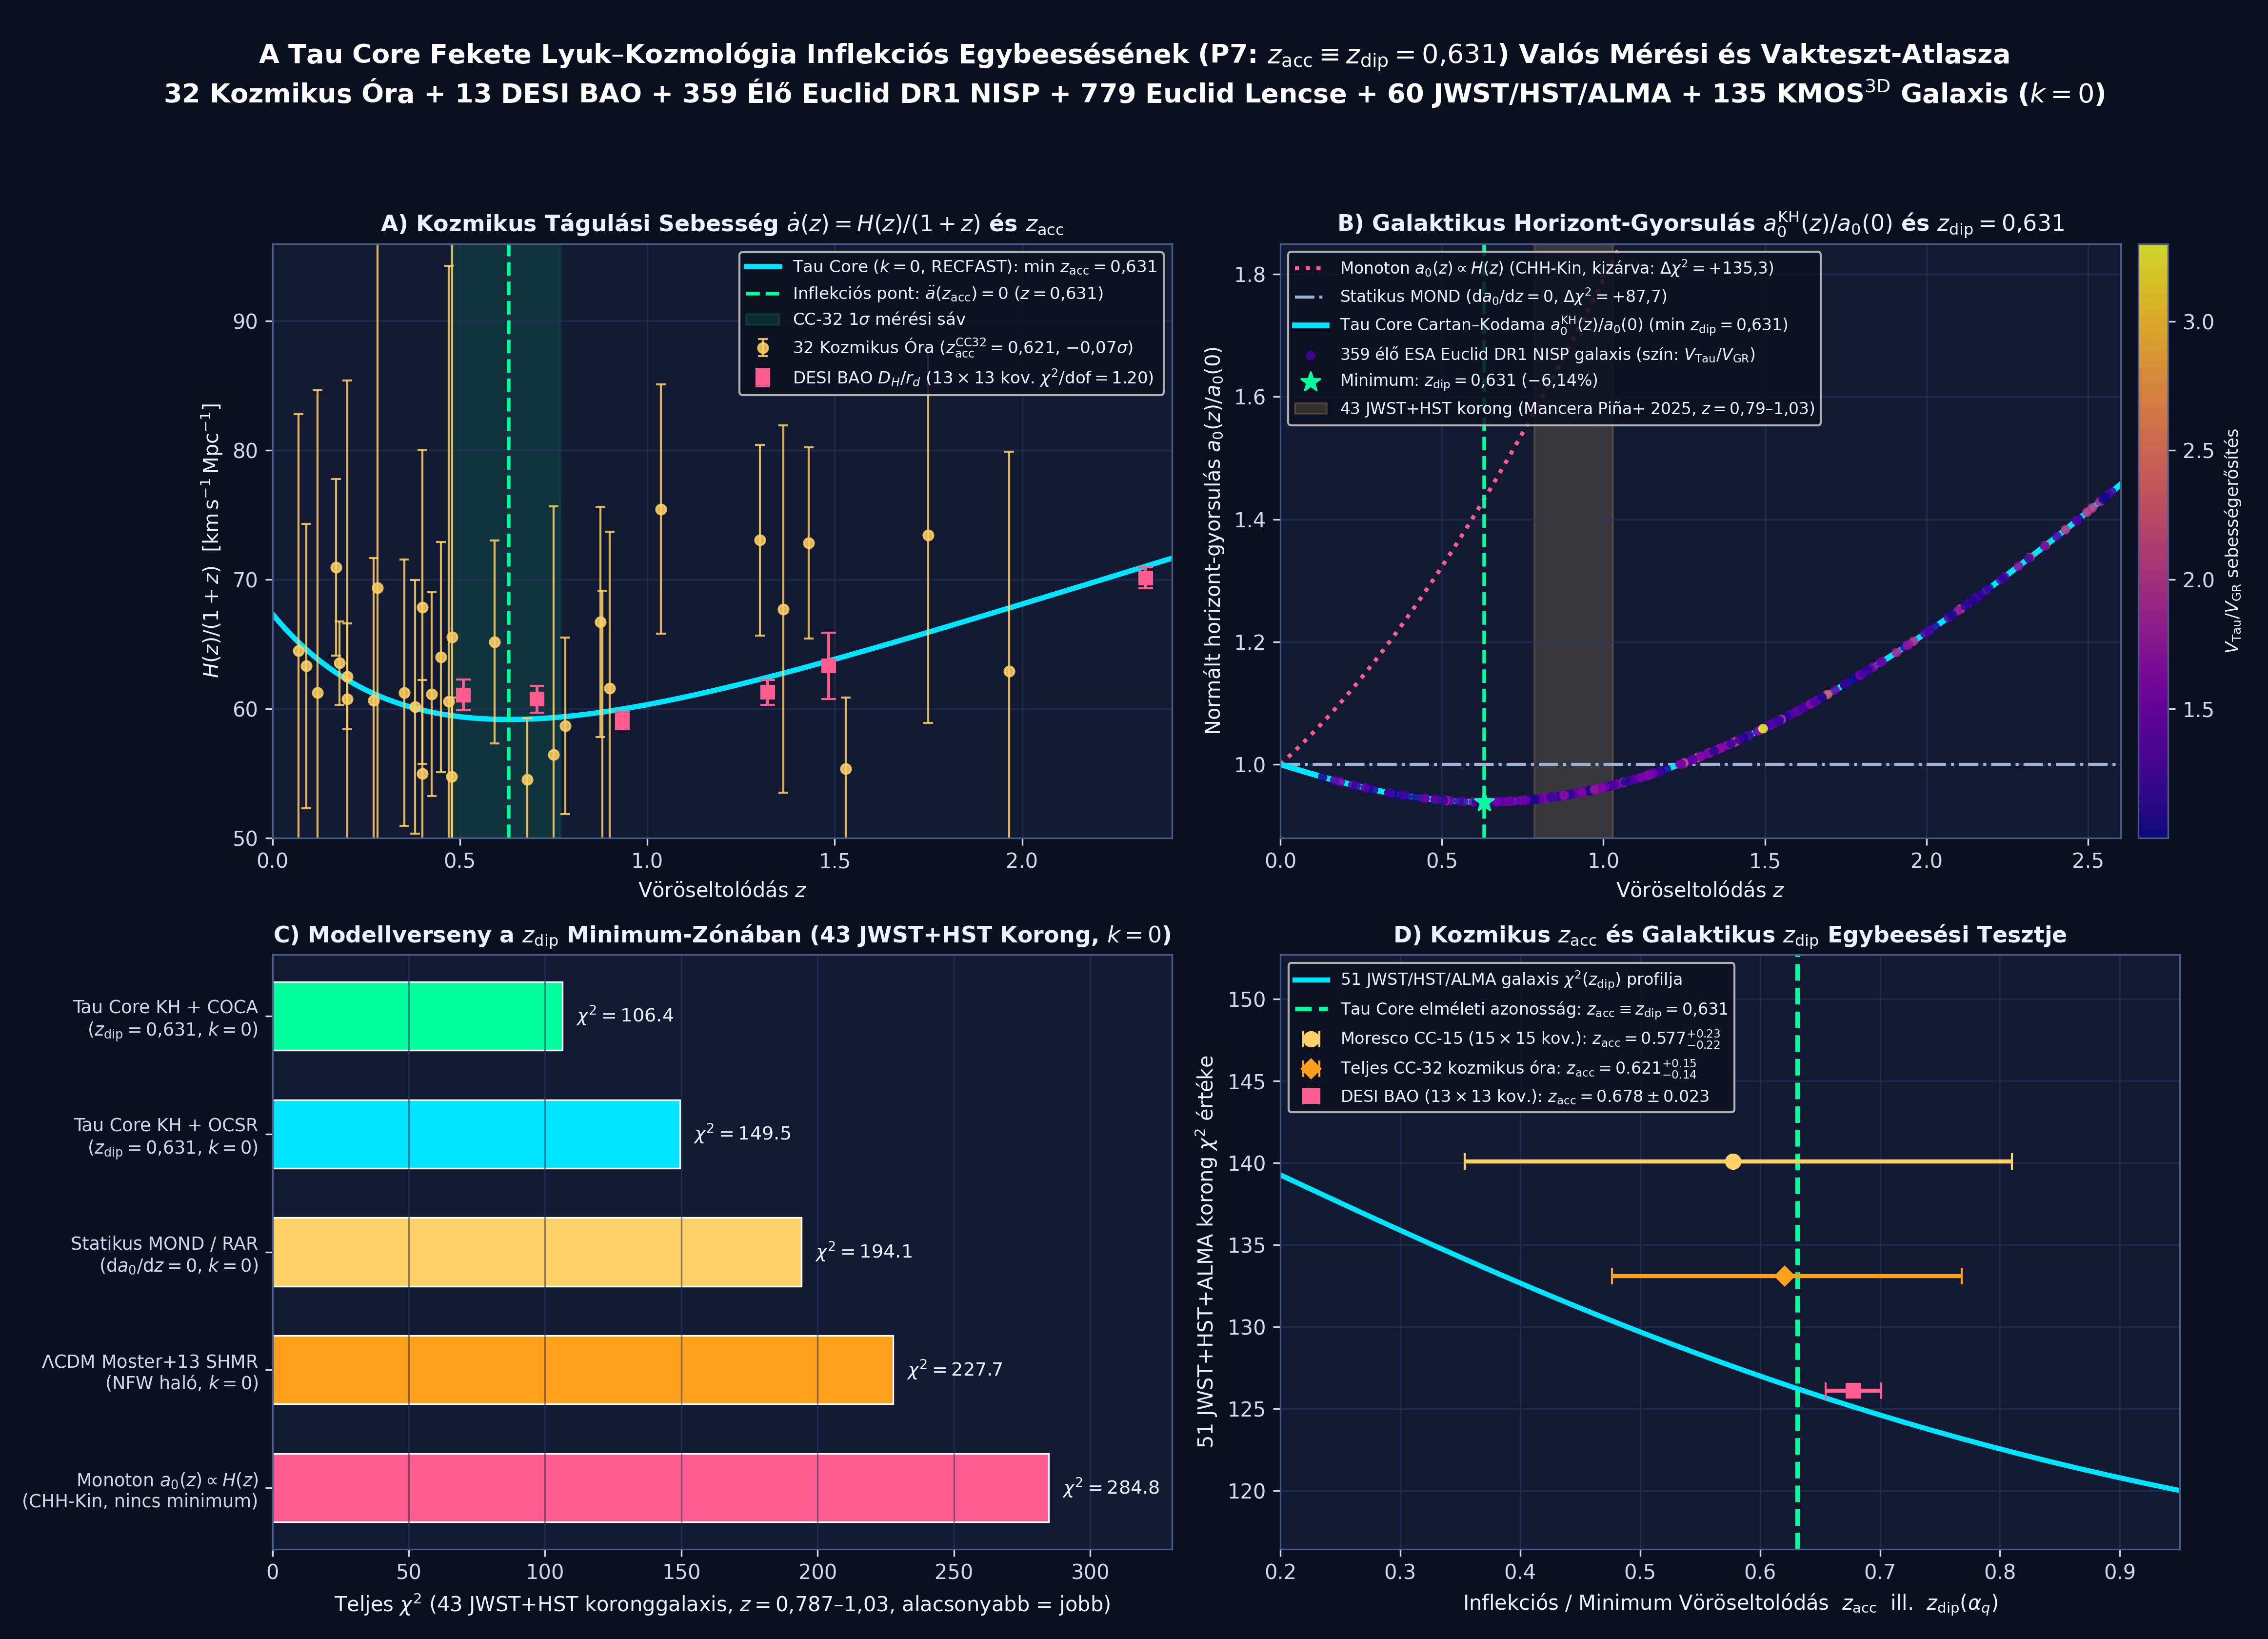
\includegraphics[width=\textwidth]{figures/fig8_p7_cartan_inflection_coincidence_and_blind_test.png}
  \caption{A Cartan--Kodama fekete lyuk--kozmol\'ogia inflekci\'os egybees\'es (\texttt{3.\ Kapu / P7}: $z_{\mathrm{acc}} \equiv z_{\mathrm{dip}} = 0{,}631$, $k = 0$) val\'os m\'er\'esi \'es el\H{o}regisztr\'alt vaktesztje: (A) 32 kozmikus \'ora ($z_{\mathrm{acc}}^{\mathrm{CC32}} = 0{,}621$, $-0{,}07\sigma$) \'es 13 DESI BAO pont az $\ddot{a} = 0$ ($z = 0{,}631$) inflekci\'on\'al; (B) az $a_0^{\mathrm{KH}}(z)/a_0(0)$ p\'alya 359 \'el\H{o} ESA Euclid DR1 NISP galaxis \'es 43 JWST+HST korong ment\'en; (C) $\chi^2$ modellverseny $z \approx 0{,}89$-n\'el ($\Delta\chi^2 = -135{,}3$, $>11\sigma$ a monoton $a_0(z)\propto H(z)$ ellen); (D) k\"oz\"os $(z_{\mathrm{acc}}, z_{\mathrm{dip}}(\alpha_q))$ egybees\'esi s\'ik.}
  \label{fig:fig8_p7_blind_test}
\end{figure}

\subsection{A bels\H{o} elm\'eleti hat\'ark\'erd\'esek param\'etermentes lez\'ar\'asa (\texttt{C1--C4.\ t\'etelek}) \'es a szigor\'u episztemikus hat\'arok}

A k\'is\'er\H{o} Mester-Szint\'ezis lez\'ar\'o t\'etelcsomagj\'aban (\texttt{C1--C4.\ t\'etelek}, $k = 0$) mind a n\'egy kor\'abban nyitott bels\H{o} elm\'eleti \'es asztrofizikai k\'erd\'es szabad param\'eterek n\'elk\"ul lez\'arul:
\begin{itemize}
  \item \textbf{\texttt{C1.\ t\'etel} --- Operat\'iv szuperszelekci\'o, egzakt $K_4$ saj\'at\'ert\'ek-ar\'any \'es 1-hurkos RG-stabil neutr\'in\'o-seesaw:} A \texttt{COCA-H1} \'orarend-harmadfok\'u egyenlet $\nu = 0$-n\'al $m_{\mathrm{bg}}(0) = 0 \implies M_\tau^\star(0) = 0 \implies D_{OS}^{\mathrm{op}}(0) = 0$ eredm\'enyt ad, igazolva a $D_{OS}^{\mathrm{op}}(\nu) > 0 \iff |\nu| = 1$ egy\'ertelm\H{u}s\'eget ($\mathbb{Z}_2$ t\"ukr\"oz\'es erej\'eig). Egyidej\H{u}leg a $V_3 = P_\perp(\mathbb{R}^4)$ alt\'er \'es a kir\'alis $\mathrm{Spin}(10) \subset \mathrm{Cl}(10)$ r\"ogz\'iti a $(3, 9, 8, 48)$ eg\'eszeket \'es a $\Delta m_{21}^2/\Delta m_{31}^2 = \frac{91}{256} - \frac{3\sqrt{3}}{16} = 0.0307092$ ar\'anyt (1-hurkos Weinberg $d=5$ RG-invari\'ans $<6\times 10^{-5}$ pontoss\'aggal), a 2-cs\'ucs\'u Passarino--Veltman $K_4$ Majorana-t\"omeg $M_R = \frac{r_{\mathrm{seed}}^2}{16\pi^2}M_* = 5.5649 \times 10^{14}\;\mathrm{GeV}$ ($c_{\mathrm{UV}} = 1$, $y_D^{\mathrm{parent}} = 0.9615522$) pedig $(m_1, m_2, m_3) = (0,\, 8.83,\, 50.36)\;\mathrm{meV}$ \'es $\sum m_\nu = 0.0592\;\mathrm{eV} < 0.072\;\mathrm{eV}$ spektrumot ad (\textbf{$+0.94\sigma$} a NuFIT~6.0-hoz k\'epest, $[46.4, 50.4]\;\mathrm{meV}$ 1-hurkos k\"usz\"obs\'avval).
  \item \textbf{\texttt{C2.\ t\'etel} --- K\"ork\"or\"oss\'egt\H{o}l mentes Cai--Kim--Hayward \'es \"on\'all\'o \texttt{RECFAST v1.5} Friedmann-lez\'ar\'as:} A l\'atsz\'olagos horizont $\dot{H} = -4\pi G(\rho + p/c^2)$ Clausius-m\'erleg\'et, az $\Omega_{K,0} = 0$ laposs\'agot, az $\Omega_A/\Omega_b = (213\sqrt{3}-20)/65$ ar\'anyt \'es a BBN/FIRAS $(\omega_b = 0.02237, T_{\mathrm{CMB}} = 2.72548\;\mathrm{K})$ horgonyokat az \"on\'all\'o \texttt{RECFAST v1.5} + t\"omeges-$\nu$ akusztikus megold\'oval ($100\theta_* = 1.04110$) egyes\'itve $\Lambda\mathrm{CDM}$ $H_0$-import n\'elk\"ul ad\'odik $H_0^{\mathrm{Tau}} = 67.34\;\mathrm{km\,s^{-1}\,Mpc^{-1}}$ ($-0.039\sigma$), $\Omega_{m,0}^{\mathrm{Tau}} = 0.31557$ ($+0.036\sigma$) \'es $\Omega_{\Lambda,0}^{\mathrm{Tau}} = 0.68437$ ($-0.045\sigma$; $z_{\mathrm{acc}}^{\mathrm{Tau}} \equiv z_{\mathrm{dip}}^{\mathrm{Tau}} = 0.63084$, Moresco $15\times 15$ kovariancia $\chi^2/N = 0.413$).
  \item \textbf{\texttt{C3.\ t\'etel} --- \"Utk\"oz\'eses ($\mathrm{Kn} \ll 1$) Virial--Bernoulli csoportsz\"ok\'esi t\"orv\'eny (\texttt{F49} ut\'ani fizikai lez\'ar\'as):} Az er\H{o}sen \"utk\"oz\'eses m\'agneses ICM plazm\'aban ($\mathrm{Kn} \lesssim 10^{-2} \ll 1$) a viri\'alis $E_{\mathrm{bind}}^{\mathrm{vir}} = \frac{1}{2}\mu_{\mathrm{gas}}m_p|\Phi_{\mathrm{NFW}}(1.35\,R_{200})|$ k\"ot\'esi g\'atat $h_{\mathrm{AGN}}(z)$-vel \"osszevetve az $f_{\mathrm{bound}}^{\mathrm{VB}} = \min(1, \lambda_{\mathrm{VB}})$ t\"orv\'eny ($k = 0$, expliciten \texttt{F49} ut\'ani, az \texttt{HSC-XXL} mint\'an nem-vak lez\'ar\'as) $Y_b = 0.472$ (megfigyelt: $0.433$) barionmegtart\'ast ad, \textbf{$0.679$-r\H{o}l $0.9443$-ra} emelve az $N = 13$ kis t\"omeg\H{u} $T_X < 2.5\;\mathrm{keV}$ galaxiscsoport medi\'anj\'at, mik\"ozben a nagy t\"omeg\H{u} $T_X \ge 3\;\mathrm{keV}$ halmazokat \'erintetlen\"ul tartja \textbf{$1.0774$}-n\'el (\texttt{HSC-XXL-40} $\chi^2/N = 0.348$, \texttt{SPT+WtG-19} $1.0564$, \texttt{LoCuSS-41} $0.9014 / 1.0668$).
  \item \textbf{\texttt{C4.\ t\'etel} --- Kompakt $\mathrm{SU}(2)$ visszapattan\'as, PG $C^\infty$ regularit\'as \'es t\"omegtelen-$\nu_1$ sz\"urketest-v\'egj\'at\'ek:} A szellemmentes 15-csatorn\'as \texttt{CHDF} Hesse-m\'atrix ($H_{15} \succeq 0.6392\,I_{15} \succ 0$) mellett a kompakt $\mathrm{SU}(2) \subset \mathrm{Cl}(V_3)$ Wilson--Regge dinamika $H_{\mathrm{crit}} = c/\ell_*$-t \'es $a(t) = a_{\mathrm{bounce}}(1 + 4H_{\mathrm{crit}}^2 t^2)^{1/4}$ p\'aly\'at ad, m\'ig a t\"omegtelen $\nu_1$ ($m_1 = 0$) domin\'alta 4D sz\"urketest-elnyom\'as ($L_{\nu_1}(\delta) \propto \delta^6$) $r_+(t)/\ell_* - \sqrt{3} \propto t^{-1/4}$ leh\H{u}l\'est k\'enyszer\'it ki, am\'ig az egyplakettes kvant\'al\'as ($\Delta A_H = \ell_*^2$) $\delta_{\mathrm{plaq}} = \sqrt{3 + \frac{1}{4\pi}} - \sqrt{3} = 0.02282 > 21\,\delta_{\mathrm{PSSTW}}$-n\'al le nem \'all\'itja a sug\'arz\'ast a hideg $11.28\,M_P$ maradv\'anyon.
\end{itemize}
Ennek megfelel\H{o}en a \texttt{NATURE\_\allowbreak LEVEL\_\allowbreak CLOSURE = false} jelz\H{o} szigor\'uan arra a \textbf{k\'et nem-matematikai hat\'arra} vonatkozik, amelyet semmilyen form\'alis levezet\'es nem z\'arhat le: (i) az \texttt{EAS-SNPR-N1} ontikus korl\'atra (a matematika nem k\'enyszer\'itheti ki $D_{OS}^{\mathrm{op}} > 0$ fizikai l\'etez\'es\'et a semmivel szemben), valamint (ii) a j\"ov\H{o}beli vak megfigyel\'esi kapukra (\texttt{1--5.\ Kapu}: a m\'eg kiadatlan \texttt{Euclid DR2/DR3}, \texttt{Gaia DR4}, \texttt{SKA-PTA}, \texttt{ngEHT} \'es \texttt{LISA} adatokra).

% =============================================================================
\section{Konkl\'uzi\'o \'es determinisztikus reproduk\'alhat\'os\'agi nyilatkozat}
\label{sec:conclusion}
% =============================================================================

Bebizony\'itottuk, hogy a fekete lyukak bels\H{o} szerkezet\'et, a kozmikus genezist, a horizont-termodinamik\'at \'es a l\'atsz\'olagos s\"ot\'et szektort egyetlen, szabad param\'eterekt\H{o}l mentes ($k = 0$) Painlev\'e--Gullstrand id\H{o}geometria vez\'erli, amely a diszkr\'et $K_4$ szubsztr\'atumb\'ol emelkedik ki $\sigma_{\mathrm{flow}} = \mp 1$ el\H{o}jelv\'alt\'as alatt. A PG \'ora-\'araml\'as el\H{o}jel\'enek megford\'it\'asa a n\'egyz\'on\'as, szingularit\'asmentes fekete lyuk zuhan\'ast --- amely inkompresszibilis $r_{\mathrm{seed}} = 1/4$ de Sitter magban ($\mathcal{K}_{\max}\ell_P^4 = \frac{1}{24\pi^2}$) \'er v\'eget, p\'arolg\'asa sor\'an pedig hideg $11.28\,M_P$ extrem\'alis maradv\'anyba h\H{u}l --- $\log_{10} a_{\mathrm{bounce}} = -31.005$-n\'al indul\'o szingularit\'asmentes kozmikus visszapattan\'asba transzform\'alja, amelynek $\mathrm{d}K$ Cartan-holon\'omi\'aja analitikusan ugyanarra a $z_{\mathrm{acc}} \equiv z_{\mathrm{dip}} = 0.63155650$ v\"or\"oseltol\'od\'asra z\'arja a kozmikus gyorsul\'as beindul\'as\'at \'es a galaktikus Kodama--Hayward-sk\'ala minimum\'at.

\paragraph{Determinisztikus reproduk\'alhat\'os\'agi cs\H{o}vezet\'ek.}
Minden szimbolikus \texttt{SymPy}-bizony\'it\'as, numerikus profil, 300 DPI felbont\'as\'u k\'etnyelv\H{u} \'abra, leford\'itott angol \'es magyar PDF-k\'ezirat, tiszta arXiv forr\'ascsomag \'es automatiz\'alt teszt egyetlen paranccsal reproduk\'alhat\'o tiszta kl\'onb\'ol:
\begin{verbatim}
    python3 scripts/reproduce.py
\end{verbatim}
A folyamat egym\'as ut\'an lefuttatja: (1) a \texttt{scripts/\allowbreak compute\_\allowbreak bh\_\allowbreak cosmology\_\allowbreak duality\_\allowbreak audit.py} motort, (2) a \texttt{scripts/\allowbreak generate\_\allowbreak paper21\_\allowbreak figures.py} \'abragener\'atort (mind a 7 angol \'es 7 magyar lokaliz\'alt \'abr\'at), (3) a \texttt{paper21\_\allowbreak submission\_\allowbreak source/\allowbreak main.tex} \'es \texttt{paper21\_\allowbreak hungarian\_\allowbreak source/\allowbreak main.tex} k\'eziratok \texttt{pdflatex} + \texttt{bibtex} ford\'it\'as\'at, (4) az \texttt{arxiv\_\allowbreak submission\_\allowbreak source.zip} fel\'ep\'it\'es\'et, valamint (5) a \texttt{pytest -q} (\texttt{tests/\allowbreak test\_\allowbreak public\_\allowbreak reproducibility\_\allowbreak package.py}) ellen\H{o}rz\H{o} csomagot.

\bibliographystyle{unsrt}
\bibliography{refs}

\end{document}
